\documentclass[twoside]{book}

% Packages required by doxygen
\usepackage{fixltx2e}
\usepackage{calc}
\usepackage{doxygen}
\usepackage[export]{adjustbox} % also loads graphicx
\usepackage{graphicx}
\usepackage[utf8]{inputenc}
\usepackage{makeidx}
\usepackage{multicol}
\usepackage{multirow}
\PassOptionsToPackage{warn}{textcomp}
\usepackage{textcomp}
\usepackage[nointegrals]{wasysym}
\usepackage[table]{xcolor}

% Font selection
\usepackage[T1]{fontenc}
\usepackage[scaled=.90]{helvet}
\usepackage{courier}
\usepackage{amssymb}
\usepackage{sectsty}
\renewcommand{\familydefault}{\sfdefault}
\allsectionsfont{%
  \fontseries{bc}\selectfont%
  \color{darkgray}%
}
\renewcommand{\DoxyLabelFont}{%
  \fontseries{bc}\selectfont%
  \color{darkgray}%
}
\newcommand{\+}{\discretionary{\mbox{\scriptsize$\hookleftarrow$}}{}{}}

% Page & text layout
\usepackage{geometry}
\geometry{%
  a4paper,%
  top=2.5cm,%
  bottom=2.5cm,%
  left=2.5cm,%
  right=2.5cm%
}
\tolerance=750
\hfuzz=15pt
\hbadness=750
\setlength{\emergencystretch}{15pt}
\setlength{\parindent}{0cm}
\setlength{\parskip}{3ex plus 2ex minus 2ex}
\makeatletter
\renewcommand{\paragraph}{%
  \@startsection{paragraph}{4}{0ex}{-1.0ex}{1.0ex}{%
    \normalfont\normalsize\bfseries\SS@parafont%
  }%
}
\renewcommand{\subparagraph}{%
  \@startsection{subparagraph}{5}{0ex}{-1.0ex}{1.0ex}{%
    \normalfont\normalsize\bfseries\SS@subparafont%
  }%
}
\makeatother

% Headers & footers
\usepackage{fancyhdr}
\pagestyle{fancyplain}
\fancyhead[LE]{\fancyplain{}{\bfseries\thepage}}
\fancyhead[CE]{\fancyplain{}{}}
\fancyhead[RE]{\fancyplain{}{\bfseries\leftmark}}
\fancyhead[LO]{\fancyplain{}{\bfseries\rightmark}}
\fancyhead[CO]{\fancyplain{}{}}
\fancyhead[RO]{\fancyplain{}{\bfseries\thepage}}
\fancyfoot[LE]{\fancyplain{}{}}
\fancyfoot[CE]{\fancyplain{}{}}
\fancyfoot[RE]{\fancyplain{}{\bfseries\scriptsize Generated by Doxygen }}
\fancyfoot[LO]{\fancyplain{}{\bfseries\scriptsize Generated by Doxygen }}
\fancyfoot[CO]{\fancyplain{}{}}
\fancyfoot[RO]{\fancyplain{}{}}
\renewcommand{\footrulewidth}{0.4pt}
\renewcommand{\chaptermark}[1]{%
  \markboth{#1}{}%
}
\renewcommand{\sectionmark}[1]{%
  \markright{\thesection\ #1}%
}

% Indices & bibliography
\usepackage{natbib}
\usepackage[titles]{tocloft}
\setcounter{tocdepth}{3}
\setcounter{secnumdepth}{5}
\makeindex

% Hyperlinks (required, but should be loaded last)
\usepackage{ifpdf}
\ifpdf
  \usepackage[pdftex,pagebackref=true]{hyperref}
\else
  \usepackage[ps2pdf,pagebackref=true]{hyperref}
\fi
\hypersetup{%
  colorlinks=true,%
  linkcolor=blue,%
  citecolor=blue,%
  unicode%
}

% Custom commands
\newcommand{\clearemptydoublepage}{%
  \newpage{\pagestyle{empty}\cleardoublepage}%
}

\usepackage{caption}
\captionsetup{labelsep=space,justification=centering,font={bf},singlelinecheck=off,skip=4pt,position=top}

%===== C O N T E N T S =====

\begin{document}

% Titlepage & ToC
\hypersetup{pageanchor=false,
             bookmarksnumbered=true,
             pdfencoding=unicode
            }
\pagenumbering{alph}
\begin{titlepage}
\vspace*{7cm}
\begin{center}%
{\Large Pedido Fácil A\+PI }\\
\vspace*{1cm}
{\large Generated by Doxygen 1.8.14}\\
\end{center}
\end{titlepage}
\clearemptydoublepage
\pagenumbering{roman}
\tableofcontents
\clearemptydoublepage
\pagenumbering{arabic}
\hypersetup{pageanchor=true}

%--- Begin generated contents ---
\chapter{Hierarchical Index}
\section{Class Hierarchy}
This inheritance list is sorted roughly, but not completely, alphabetically\+:\begin{DoxyCompactList}
\item \contentsline{section}{Additional\+Repository\+Interface}{\pageref{interface_app_1_1_repositories_1_1_product_1_1_additional_repository_interface}}{}
\item \contentsline{section}{Authenticate}{\pageref{class_app_1_1_http_1_1_middleware_1_1_authenticate}}{}
\item Base\+Controller\begin{DoxyCompactList}
\item \contentsline{section}{Controller}{\pageref{class_app_1_1_http_1_1_controllers_1_1_controller}}{}
\begin{DoxyCompactList}
\item \contentsline{section}{Card\+Controller}{\pageref{class_app_1_1_http_1_1_controllers_1_1_card_controller}}{}
\item \contentsline{section}{Order\+Controller}{\pageref{class_app_1_1_http_1_1_controllers_1_1_order_controller}}{}
\item \contentsline{section}{Additional\+Controller}{\pageref{class_app_1_1_http_1_1_controllers_1_1_product_1_1_additional_controller}}{}
\item \contentsline{section}{Category\+Controller}{\pageref{class_app_1_1_http_1_1_controllers_1_1_product_1_1_category_controller}}{}
\item \contentsline{section}{Group\+Controller}{\pageref{class_app_1_1_http_1_1_controllers_1_1_product_1_1_group_controller}}{}
\item \contentsline{section}{Ingredient\+Controller}{\pageref{class_app_1_1_http_1_1_controllers_1_1_product_1_1_ingredient_controller}}{}
\item \contentsline{section}{Product\+Controller}{\pageref{class_app_1_1_http_1_1_controllers_1_1_product_1_1_product_controller}}{}
\item \contentsline{section}{Table\+Controller}{\pageref{class_app_1_1_http_1_1_controllers_1_1_table_controller}}{}
\item \contentsline{section}{User\+Controller}{\pageref{class_app_1_1_http_1_1_controllers_1_1_user_controller}}{}
\item \contentsline{section}{Waiter\+Controller}{\pageref{class_app_1_1_http_1_1_controllers_1_1_waiter_controller}}{}
\end{DoxyCompactList}
\end{DoxyCompactList}
\item \contentsline{section}{Category\+Repository\+Interface}{\pageref{interface_app_1_1_repositories_1_1_product_1_1_category_repository_interface}}{}
\item Console\+Kernel\begin{DoxyCompactList}
\item \contentsline{section}{Kernel}{\pageref{class_app_1_1_console_1_1_kernel}}{}
\end{DoxyCompactList}
\item \contentsline{section}{Example\+Middleware}{\pageref{class_app_1_1_http_1_1_middleware_1_1_example_middleware}}{}
\item Exception\+Handler\begin{DoxyCompactList}
\item \contentsline{section}{Handler}{\pageref{class_app_1_1_exceptions_1_1_handler}}{}
\end{DoxyCompactList}
\item \contentsline{section}{Group\+Repository\+Interface}{\pageref{interface_app_1_1_repositories_1_1_product_1_1_group_repository_interface}}{}
\item \contentsline{section}{Ingredient\+Repository\+Interface}{\pageref{interface_app_1_1_repositories_1_1_product_1_1_ingredient_repository_interface}}{}
\item \contentsline{section}{Product\+Repository\+Interface}{\pageref{interface_app_1_1_repositories_1_1_product_1_1_product_repository_interface}}{}
\item Model\begin{DoxyCompactList}
\item \contentsline{section}{Card}{\pageref{class_app_1_1_models_1_1_card}}{}
\item \contentsline{section}{Order}{\pageref{class_app_1_1_models_1_1_order}}{}
\item \contentsline{section}{Additional}{\pageref{class_app_1_1_models_1_1_product_1_1_additional}}{}
\item \contentsline{section}{Category}{\pageref{class_app_1_1_models_1_1_product_1_1_category}}{}
\item \contentsline{section}{Group}{\pageref{class_app_1_1_models_1_1_product_1_1_group}}{}
\item \contentsline{section}{Ingredient}{\pageref{class_app_1_1_models_1_1_product_1_1_ingredient}}{}
\item \contentsline{section}{Product}{\pageref{class_app_1_1_models_1_1_product_1_1_product}}{}
\item \contentsline{section}{Table}{\pageref{class_app_1_1_models_1_1_table}}{}
\item \contentsline{section}{User}{\pageref{class_app_1_1_models_1_1_user}}{}
\item \contentsline{section}{Waiter}{\pageref{class_app_1_1_models_1_1_waiter}}{}
\end{DoxyCompactList}
\item Service\+Provider\begin{DoxyCompactList}
\item \contentsline{section}{App\+Service\+Provider}{\pageref{class_app_1_1_providers_1_1_app_service_provider}}{}
\item \contentsline{section}{Auth\+Service\+Provider}{\pageref{class_app_1_1_providers_1_1_auth_service_provider}}{}
\item \contentsline{section}{Event\+Service\+Provider}{\pageref{class_app_1_1_providers_1_1_event_service_provider}}{}
\end{DoxyCompactList}
\end{DoxyCompactList}

\chapter{Data Structure Index}
\section{Data Structures}
Here are the data structures with brief descriptions\+:\begin{DoxyCompactList}
\item\contentsline{section}{\mbox{\hyperlink{class_app_1_1_models_1_1_product_1_1_additional}{Additional}} }{\pageref{class_app_1_1_models_1_1_product_1_1_additional}}{}
\item\contentsline{section}{\mbox{\hyperlink{class_app_1_1_http_1_1_controllers_1_1_product_1_1_additional_controller}{Additional\+Controller}} }{\pageref{class_app_1_1_http_1_1_controllers_1_1_product_1_1_additional_controller}}{}
\item\contentsline{section}{\mbox{\hyperlink{interface_app_1_1_repositories_1_1_product_1_1_additional_repository_interface}{Additional\+Repository\+Interface}} }{\pageref{interface_app_1_1_repositories_1_1_product_1_1_additional_repository_interface}}{}
\item\contentsline{section}{\mbox{\hyperlink{class_app_1_1_providers_1_1_app_service_provider}{App\+Service\+Provider}} }{\pageref{class_app_1_1_providers_1_1_app_service_provider}}{}
\item\contentsline{section}{\mbox{\hyperlink{class_app_1_1_http_1_1_middleware_1_1_authenticate}{Authenticate}} }{\pageref{class_app_1_1_http_1_1_middleware_1_1_authenticate}}{}
\item\contentsline{section}{\mbox{\hyperlink{class_app_1_1_providers_1_1_auth_service_provider}{Auth\+Service\+Provider}} }{\pageref{class_app_1_1_providers_1_1_auth_service_provider}}{}
\item\contentsline{section}{\mbox{\hyperlink{class_app_1_1_models_1_1_card}{Card}} }{\pageref{class_app_1_1_models_1_1_card}}{}
\item\contentsline{section}{\mbox{\hyperlink{class_app_1_1_http_1_1_controllers_1_1_card_controller}{Card\+Controller}} }{\pageref{class_app_1_1_http_1_1_controllers_1_1_card_controller}}{}
\item\contentsline{section}{\mbox{\hyperlink{class_app_1_1_models_1_1_product_1_1_category}{Category}} }{\pageref{class_app_1_1_models_1_1_product_1_1_category}}{}
\item\contentsline{section}{\mbox{\hyperlink{class_app_1_1_http_1_1_controllers_1_1_product_1_1_category_controller}{Category\+Controller}} }{\pageref{class_app_1_1_http_1_1_controllers_1_1_product_1_1_category_controller}}{}
\item\contentsline{section}{\mbox{\hyperlink{interface_app_1_1_repositories_1_1_product_1_1_category_repository_interface}{Category\+Repository\+Interface}} }{\pageref{interface_app_1_1_repositories_1_1_product_1_1_category_repository_interface}}{}
\item\contentsline{section}{\mbox{\hyperlink{class_app_1_1_http_1_1_controllers_1_1_controller}{Controller}} }{\pageref{class_app_1_1_http_1_1_controllers_1_1_controller}}{}
\item\contentsline{section}{\mbox{\hyperlink{class_app_1_1_providers_1_1_event_service_provider}{Event\+Service\+Provider}} }{\pageref{class_app_1_1_providers_1_1_event_service_provider}}{}
\item\contentsline{section}{\mbox{\hyperlink{class_app_1_1_http_1_1_middleware_1_1_example_middleware}{Example\+Middleware}} }{\pageref{class_app_1_1_http_1_1_middleware_1_1_example_middleware}}{}
\item\contentsline{section}{\mbox{\hyperlink{class_app_1_1_models_1_1_product_1_1_group}{Group}} }{\pageref{class_app_1_1_models_1_1_product_1_1_group}}{}
\item\contentsline{section}{\mbox{\hyperlink{class_app_1_1_http_1_1_controllers_1_1_product_1_1_group_controller}{Group\+Controller}} }{\pageref{class_app_1_1_http_1_1_controllers_1_1_product_1_1_group_controller}}{}
\item\contentsline{section}{\mbox{\hyperlink{interface_app_1_1_repositories_1_1_product_1_1_group_repository_interface}{Group\+Repository\+Interface}} }{\pageref{interface_app_1_1_repositories_1_1_product_1_1_group_repository_interface}}{}
\item\contentsline{section}{\mbox{\hyperlink{class_app_1_1_exceptions_1_1_handler}{Handler}} }{\pageref{class_app_1_1_exceptions_1_1_handler}}{}
\item\contentsline{section}{\mbox{\hyperlink{class_app_1_1_models_1_1_product_1_1_ingredient}{Ingredient}} }{\pageref{class_app_1_1_models_1_1_product_1_1_ingredient}}{}
\item\contentsline{section}{\mbox{\hyperlink{class_app_1_1_http_1_1_controllers_1_1_product_1_1_ingredient_controller}{Ingredient\+Controller}} }{\pageref{class_app_1_1_http_1_1_controllers_1_1_product_1_1_ingredient_controller}}{}
\item\contentsline{section}{\mbox{\hyperlink{interface_app_1_1_repositories_1_1_product_1_1_ingredient_repository_interface}{Ingredient\+Repository\+Interface}} }{\pageref{interface_app_1_1_repositories_1_1_product_1_1_ingredient_repository_interface}}{}
\item\contentsline{section}{\mbox{\hyperlink{class_app_1_1_console_1_1_kernel}{Kernel}} }{\pageref{class_app_1_1_console_1_1_kernel}}{}
\item\contentsline{section}{\mbox{\hyperlink{class_app_1_1_models_1_1_order}{Order}} }{\pageref{class_app_1_1_models_1_1_order}}{}
\item\contentsline{section}{\mbox{\hyperlink{class_app_1_1_http_1_1_controllers_1_1_order_controller}{Order\+Controller}} }{\pageref{class_app_1_1_http_1_1_controllers_1_1_order_controller}}{}
\item\contentsline{section}{\mbox{\hyperlink{class_app_1_1_models_1_1_product_1_1_product}{Product}} }{\pageref{class_app_1_1_models_1_1_product_1_1_product}}{}
\item\contentsline{section}{\mbox{\hyperlink{class_app_1_1_http_1_1_controllers_1_1_product_1_1_product_controller}{Product\+Controller}} }{\pageref{class_app_1_1_http_1_1_controllers_1_1_product_1_1_product_controller}}{}
\item\contentsline{section}{\mbox{\hyperlink{interface_app_1_1_repositories_1_1_product_1_1_product_repository_interface}{Product\+Repository\+Interface}} }{\pageref{interface_app_1_1_repositories_1_1_product_1_1_product_repository_interface}}{}
\item\contentsline{section}{\mbox{\hyperlink{class_app_1_1_models_1_1_table}{Table}} }{\pageref{class_app_1_1_models_1_1_table}}{}
\item\contentsline{section}{\mbox{\hyperlink{class_app_1_1_http_1_1_controllers_1_1_table_controller}{Table\+Controller}} }{\pageref{class_app_1_1_http_1_1_controllers_1_1_table_controller}}{}
\item\contentsline{section}{\mbox{\hyperlink{class_app_1_1_models_1_1_user}{User}} }{\pageref{class_app_1_1_models_1_1_user}}{}
\item\contentsline{section}{\mbox{\hyperlink{class_app_1_1_http_1_1_controllers_1_1_user_controller}{User\+Controller}} }{\pageref{class_app_1_1_http_1_1_controllers_1_1_user_controller}}{}
\item\contentsline{section}{\mbox{\hyperlink{class_app_1_1_models_1_1_waiter}{Waiter}} }{\pageref{class_app_1_1_models_1_1_waiter}}{}
\item\contentsline{section}{\mbox{\hyperlink{class_app_1_1_http_1_1_controllers_1_1_waiter_controller}{Waiter\+Controller}} }{\pageref{class_app_1_1_http_1_1_controllers_1_1_waiter_controller}}{}
\end{DoxyCompactList}

\chapter{Data Structure Documentation}
\hypertarget{class_app_1_1_models_1_1_product_1_1_additional}{}\section{Additional Class Reference}
\label{class_app_1_1_models_1_1_product_1_1_additional}\index{Additional@{Additional}}


Inheritance diagram for Additional\+:
\nopagebreak
\begin{figure}[H]
\begin{center}
\leavevmode
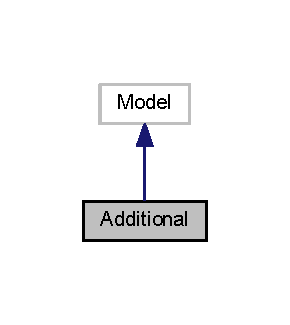
\includegraphics[width=139pt]{class_app_1_1_models_1_1_product_1_1_additional__inherit__graph}
\end{center}
\end{figure}


Collaboration diagram for Additional\+:
\nopagebreak
\begin{figure}[H]
\begin{center}
\leavevmode
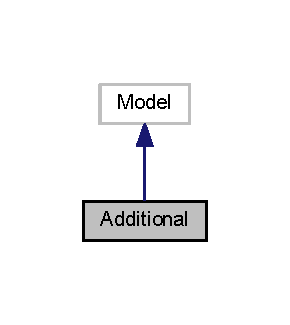
\includegraphics[width=139pt]{class_app_1_1_models_1_1_product_1_1_additional__coll__graph}
\end{center}
\end{figure}
\subsection*{Protected Attributes}
\begin{DoxyCompactItemize}
\item 
\mbox{\Hypertarget{class_app_1_1_models_1_1_product_1_1_additional_ae8876a14058f368335baccf35af4a22b}\label{class_app_1_1_models_1_1_product_1_1_additional_ae8876a14058f368335baccf35af4a22b}} 
{\bfseries \$table} = \textquotesingle{}product\+\_\+additionals\textquotesingle{}
\item 
{\bfseries \$fillabe}
\end{DoxyCompactItemize}


\subsection{Detailed Description}
Class that represent the additionals a product can have. Could be double meat, double cheese, lemon and ice.

Accepts name\+: string, price\+: double, status\+: tiny\+Integer. Status will be indicate if the ingredient is available in stock. 

\subsection{Field Documentation}
\mbox{\Hypertarget{class_app_1_1_models_1_1_product_1_1_additional_ac5c29ce22e45a54200f88204e498d290}\label{class_app_1_1_models_1_1_product_1_1_additional_ac5c29ce22e45a54200f88204e498d290}} 
\index{App\+::\+Models\+::\+Product\+::\+Additional@{App\+::\+Models\+::\+Product\+::\+Additional}!\$fillabe@{\$fillabe}}
\index{\$fillabe@{\$fillabe}!App\+::\+Models\+::\+Product\+::\+Additional@{App\+::\+Models\+::\+Product\+::\+Additional}}
\subsubsection{\texorpdfstring{\$fillabe}{$fillabe}}
{\footnotesize\ttfamily \$fillabe\hspace{0.3cm}{\ttfamily [protected]}}

{\bfseries Initial value\+:}
\begin{DoxyCode}
= [
        \textcolor{stringliteral}{'name'},
        \textcolor{stringliteral}{'price'},
        \textcolor{stringliteral}{'status'}
    ]
\end{DoxyCode}


The documentation for this class was generated from the following file\+:\begin{DoxyCompactItemize}
\item 
app/\+Models/\+Product/Additional.\+php\end{DoxyCompactItemize}

\hypertarget{class_app_1_1_http_1_1_controllers_1_1_product_1_1_additional_controller}{}\section{Additional\+Controller Class Reference}
\label{class_app_1_1_http_1_1_controllers_1_1_product_1_1_additional_controller}\index{Additional\+Controller@{Additional\+Controller}}


Inheritance diagram for Additional\+Controller\+:
\nopagebreak
\begin{figure}[H]
\begin{center}
\leavevmode
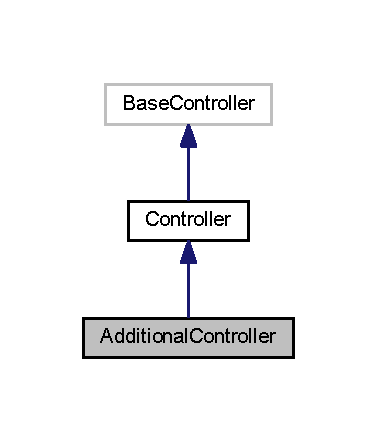
\includegraphics[width=181pt]{class_app_1_1_http_1_1_controllers_1_1_product_1_1_additional_controller__inherit__graph}
\end{center}
\end{figure}


Collaboration diagram for Additional\+Controller\+:
\nopagebreak
\begin{figure}[H]
\begin{center}
\leavevmode
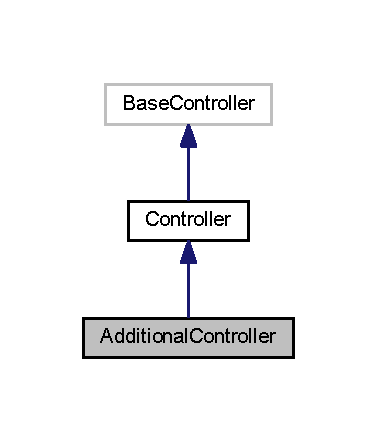
\includegraphics[width=181pt]{class_app_1_1_http_1_1_controllers_1_1_product_1_1_additional_controller__coll__graph}
\end{center}
\end{figure}
\subsection*{Public Member Functions}
\begin{DoxyCompactItemize}
\item 
\mbox{\hyperlink{class_app_1_1_http_1_1_controllers_1_1_product_1_1_additional_controller_a5b75ba6bc9debb999c0186a31978ec03}{\+\_\+\+\_\+construct}} (\$repository)
\item 
\mbox{\hyperlink{class_app_1_1_http_1_1_controllers_1_1_product_1_1_additional_controller_af9d14e4ae6227970ad603987781573ca}{all}} ()
\item 
\mbox{\hyperlink{class_app_1_1_http_1_1_controllers_1_1_product_1_1_additional_controller_a50e3bfb586b2f42932a6a93f3fbb0828}{get}} (\$id)
\item 
\mbox{\hyperlink{class_app_1_1_http_1_1_controllers_1_1_product_1_1_additional_controller_a4fa811c83f27da01b0d92bdb2a711a13}{create}} (\$request)
\item 
\mbox{\hyperlink{class_app_1_1_http_1_1_controllers_1_1_product_1_1_additional_controller_ab7b27a90191560dcef32126b0945db0d}{update}} (\$request)
\item 
\mbox{\hyperlink{class_app_1_1_http_1_1_controllers_1_1_product_1_1_additional_controller_a126a3799c44d72393ca4732081306dfd}{delete}} (\$request)
\end{DoxyCompactItemize}


\subsection{Detailed Description}
\mbox{\hyperlink{class_app_1_1_http_1_1_controllers_1_1_controller}{Controller}} for the product additionals. 

\subsection{Constructor \& Destructor Documentation}
\mbox{\Hypertarget{class_app_1_1_http_1_1_controllers_1_1_product_1_1_additional_controller_a5b75ba6bc9debb999c0186a31978ec03}\label{class_app_1_1_http_1_1_controllers_1_1_product_1_1_additional_controller_a5b75ba6bc9debb999c0186a31978ec03}} 
\index{App\+::\+Http\+::\+Controllers\+::\+Product\+::\+Additional\+Controller@{App\+::\+Http\+::\+Controllers\+::\+Product\+::\+Additional\+Controller}!\+\_\+\+\_\+construct@{\+\_\+\+\_\+construct}}
\index{\+\_\+\+\_\+construct@{\+\_\+\+\_\+construct}!App\+::\+Http\+::\+Controllers\+::\+Product\+::\+Additional\+Controller@{App\+::\+Http\+::\+Controllers\+::\+Product\+::\+Additional\+Controller}}
\subsubsection{\texorpdfstring{\+\_\+\+\_\+construct()}{\_\_construct()}}
{\footnotesize\ttfamily \+\_\+\+\_\+construct (\begin{DoxyParamCaption}\item[{}]{\$repository }\end{DoxyParamCaption})}

Using dependency injection to get the repository connected to the A\+PI in the app\+\_\+providers.


\begin{DoxyParams}[1]{Parameters}
interface & {\em \$repository} & \\
\hline
\end{DoxyParams}


\subsection{Member Function Documentation}
\mbox{\Hypertarget{class_app_1_1_http_1_1_controllers_1_1_product_1_1_additional_controller_af9d14e4ae6227970ad603987781573ca}\label{class_app_1_1_http_1_1_controllers_1_1_product_1_1_additional_controller_af9d14e4ae6227970ad603987781573ca}} 
\index{App\+::\+Http\+::\+Controllers\+::\+Product\+::\+Additional\+Controller@{App\+::\+Http\+::\+Controllers\+::\+Product\+::\+Additional\+Controller}!all@{all}}
\index{all@{all}!App\+::\+Http\+::\+Controllers\+::\+Product\+::\+Additional\+Controller@{App\+::\+Http\+::\+Controllers\+::\+Product\+::\+Additional\+Controller}}
\subsubsection{\texorpdfstring{all()}{all()}}
{\footnotesize\ttfamily all (\begin{DoxyParamCaption}{ }\end{DoxyParamCaption})}

Returns an array of Additional objects.

\begin{DoxyReturn}{Returns}
array 
\end{DoxyReturn}
\mbox{\Hypertarget{class_app_1_1_http_1_1_controllers_1_1_product_1_1_additional_controller_a4fa811c83f27da01b0d92bdb2a711a13}\label{class_app_1_1_http_1_1_controllers_1_1_product_1_1_additional_controller_a4fa811c83f27da01b0d92bdb2a711a13}} 
\index{App\+::\+Http\+::\+Controllers\+::\+Product\+::\+Additional\+Controller@{App\+::\+Http\+::\+Controllers\+::\+Product\+::\+Additional\+Controller}!create@{create}}
\index{create@{create}!App\+::\+Http\+::\+Controllers\+::\+Product\+::\+Additional\+Controller@{App\+::\+Http\+::\+Controllers\+::\+Product\+::\+Additional\+Controller}}
\subsubsection{\texorpdfstring{create()}{create()}}
{\footnotesize\ttfamily create (\begin{DoxyParamCaption}\item[{}]{\$request }\end{DoxyParamCaption})}

Store a new additional.

\begin{DoxyReturn}{Returns}
boolean 
\end{DoxyReturn}
\mbox{\Hypertarget{class_app_1_1_http_1_1_controllers_1_1_product_1_1_additional_controller_a126a3799c44d72393ca4732081306dfd}\label{class_app_1_1_http_1_1_controllers_1_1_product_1_1_additional_controller_a126a3799c44d72393ca4732081306dfd}} 
\index{App\+::\+Http\+::\+Controllers\+::\+Product\+::\+Additional\+Controller@{App\+::\+Http\+::\+Controllers\+::\+Product\+::\+Additional\+Controller}!delete@{delete}}
\index{delete@{delete}!App\+::\+Http\+::\+Controllers\+::\+Product\+::\+Additional\+Controller@{App\+::\+Http\+::\+Controllers\+::\+Product\+::\+Additional\+Controller}}
\subsubsection{\texorpdfstring{delete()}{delete()}}
{\footnotesize\ttfamily delete (\begin{DoxyParamCaption}\item[{}]{\$request }\end{DoxyParamCaption})}

Delete an additional.

\begin{DoxyReturn}{Returns}
boolean 
\end{DoxyReturn}
\mbox{\Hypertarget{class_app_1_1_http_1_1_controllers_1_1_product_1_1_additional_controller_a50e3bfb586b2f42932a6a93f3fbb0828}\label{class_app_1_1_http_1_1_controllers_1_1_product_1_1_additional_controller_a50e3bfb586b2f42932a6a93f3fbb0828}} 
\index{App\+::\+Http\+::\+Controllers\+::\+Product\+::\+Additional\+Controller@{App\+::\+Http\+::\+Controllers\+::\+Product\+::\+Additional\+Controller}!get@{get}}
\index{get@{get}!App\+::\+Http\+::\+Controllers\+::\+Product\+::\+Additional\+Controller@{App\+::\+Http\+::\+Controllers\+::\+Product\+::\+Additional\+Controller}}
\subsubsection{\texorpdfstring{get()}{get()}}
{\footnotesize\ttfamily get (\begin{DoxyParamCaption}\item[{}]{\$id }\end{DoxyParamCaption})}

Returns an Additional Object with the provided id.

\begin{DoxyReturn}{Returns}
object 
\end{DoxyReturn}
\mbox{\Hypertarget{class_app_1_1_http_1_1_controllers_1_1_product_1_1_additional_controller_ab7b27a90191560dcef32126b0945db0d}\label{class_app_1_1_http_1_1_controllers_1_1_product_1_1_additional_controller_ab7b27a90191560dcef32126b0945db0d}} 
\index{App\+::\+Http\+::\+Controllers\+::\+Product\+::\+Additional\+Controller@{App\+::\+Http\+::\+Controllers\+::\+Product\+::\+Additional\+Controller}!update@{update}}
\index{update@{update}!App\+::\+Http\+::\+Controllers\+::\+Product\+::\+Additional\+Controller@{App\+::\+Http\+::\+Controllers\+::\+Product\+::\+Additional\+Controller}}
\subsubsection{\texorpdfstring{update()}{update()}}
{\footnotesize\ttfamily update (\begin{DoxyParamCaption}\item[{}]{\$request }\end{DoxyParamCaption})}

Update an additional.

\begin{DoxyReturn}{Returns}
boolean 
\end{DoxyReturn}


The documentation for this class was generated from the following file\+:\begin{DoxyCompactItemize}
\item 
app/\+Http/\+Controllers/\+Product/Additional\+Controller.\+php\end{DoxyCompactItemize}

\hypertarget{interface_app_1_1_repositories_1_1_product_1_1_additional_repository_interface}{}\section{Additional\+Repository\+Interface Interface Reference}
\label{interface_app_1_1_repositories_1_1_product_1_1_additional_repository_interface}\index{Additional\+Repository\+Interface@{Additional\+Repository\+Interface}}
\subsection*{Public Member Functions}
\begin{DoxyCompactItemize}
\item 
\mbox{\hyperlink{interface_app_1_1_repositories_1_1_product_1_1_additional_repository_interface_af9d14e4ae6227970ad603987781573ca}{all}} ()
\item 
\mbox{\hyperlink{interface_app_1_1_repositories_1_1_product_1_1_additional_repository_interface_a50e3bfb586b2f42932a6a93f3fbb0828}{get}} (\$id)
\item 
\mbox{\hyperlink{interface_app_1_1_repositories_1_1_product_1_1_additional_repository_interface_a4fa811c83f27da01b0d92bdb2a711a13}{create}} (\$request)
\item 
\mbox{\hyperlink{interface_app_1_1_repositories_1_1_product_1_1_additional_repository_interface_a2aedea52c52e54ba3c4c9f60423e7ef1}{udpate}} (\$request)
\item 
\mbox{\hyperlink{interface_app_1_1_repositories_1_1_product_1_1_additional_repository_interface_a126a3799c44d72393ca4732081306dfd}{delete}} (\$request)
\end{DoxyCompactItemize}


\subsection{Detailed Description}
Interface for the Additional\+Repository 

\subsection{Member Function Documentation}
\mbox{\Hypertarget{interface_app_1_1_repositories_1_1_product_1_1_additional_repository_interface_af9d14e4ae6227970ad603987781573ca}\label{interface_app_1_1_repositories_1_1_product_1_1_additional_repository_interface_af9d14e4ae6227970ad603987781573ca}} 
\index{App\+::\+Repositories\+::\+Product\+::\+Additional\+Repository\+Interface@{App\+::\+Repositories\+::\+Product\+::\+Additional\+Repository\+Interface}!all@{all}}
\index{all@{all}!App\+::\+Repositories\+::\+Product\+::\+Additional\+Repository\+Interface@{App\+::\+Repositories\+::\+Product\+::\+Additional\+Repository\+Interface}}
\subsubsection{\texorpdfstring{all()}{all()}}
{\footnotesize\ttfamily all (\begin{DoxyParamCaption}{ }\end{DoxyParamCaption})}

Returns an array of Additional objects.

\begin{DoxyReturn}{Returns}
array 
\end{DoxyReturn}
\mbox{\Hypertarget{interface_app_1_1_repositories_1_1_product_1_1_additional_repository_interface_a4fa811c83f27da01b0d92bdb2a711a13}\label{interface_app_1_1_repositories_1_1_product_1_1_additional_repository_interface_a4fa811c83f27da01b0d92bdb2a711a13}} 
\index{App\+::\+Repositories\+::\+Product\+::\+Additional\+Repository\+Interface@{App\+::\+Repositories\+::\+Product\+::\+Additional\+Repository\+Interface}!create@{create}}
\index{create@{create}!App\+::\+Repositories\+::\+Product\+::\+Additional\+Repository\+Interface@{App\+::\+Repositories\+::\+Product\+::\+Additional\+Repository\+Interface}}
\subsubsection{\texorpdfstring{create()}{create()}}
{\footnotesize\ttfamily create (\begin{DoxyParamCaption}\item[{}]{\$request }\end{DoxyParamCaption})}

Returns a boolean reflecting the creation status.

\begin{DoxyReturn}{Returns}
boolean 
\end{DoxyReturn}
\mbox{\Hypertarget{interface_app_1_1_repositories_1_1_product_1_1_additional_repository_interface_a126a3799c44d72393ca4732081306dfd}\label{interface_app_1_1_repositories_1_1_product_1_1_additional_repository_interface_a126a3799c44d72393ca4732081306dfd}} 
\index{App\+::\+Repositories\+::\+Product\+::\+Additional\+Repository\+Interface@{App\+::\+Repositories\+::\+Product\+::\+Additional\+Repository\+Interface}!delete@{delete}}
\index{delete@{delete}!App\+::\+Repositories\+::\+Product\+::\+Additional\+Repository\+Interface@{App\+::\+Repositories\+::\+Product\+::\+Additional\+Repository\+Interface}}
\subsubsection{\texorpdfstring{delete()}{delete()}}
{\footnotesize\ttfamily delete (\begin{DoxyParamCaption}\item[{}]{\$request }\end{DoxyParamCaption})}

Returns a boolean reflecting the deletion status.

\begin{DoxyReturn}{Returns}
boolean 
\end{DoxyReturn}
\mbox{\Hypertarget{interface_app_1_1_repositories_1_1_product_1_1_additional_repository_interface_a50e3bfb586b2f42932a6a93f3fbb0828}\label{interface_app_1_1_repositories_1_1_product_1_1_additional_repository_interface_a50e3bfb586b2f42932a6a93f3fbb0828}} 
\index{App\+::\+Repositories\+::\+Product\+::\+Additional\+Repository\+Interface@{App\+::\+Repositories\+::\+Product\+::\+Additional\+Repository\+Interface}!get@{get}}
\index{get@{get}!App\+::\+Repositories\+::\+Product\+::\+Additional\+Repository\+Interface@{App\+::\+Repositories\+::\+Product\+::\+Additional\+Repository\+Interface}}
\subsubsection{\texorpdfstring{get()}{get()}}
{\footnotesize\ttfamily get (\begin{DoxyParamCaption}\item[{}]{\$id }\end{DoxyParamCaption})}

Returns an Additional Object with the provided id.

\begin{DoxyReturn}{Returns}
object 
\end{DoxyReturn}
\mbox{\Hypertarget{interface_app_1_1_repositories_1_1_product_1_1_additional_repository_interface_a2aedea52c52e54ba3c4c9f60423e7ef1}\label{interface_app_1_1_repositories_1_1_product_1_1_additional_repository_interface_a2aedea52c52e54ba3c4c9f60423e7ef1}} 
\index{App\+::\+Repositories\+::\+Product\+::\+Additional\+Repository\+Interface@{App\+::\+Repositories\+::\+Product\+::\+Additional\+Repository\+Interface}!udpate@{udpate}}
\index{udpate@{udpate}!App\+::\+Repositories\+::\+Product\+::\+Additional\+Repository\+Interface@{App\+::\+Repositories\+::\+Product\+::\+Additional\+Repository\+Interface}}
\subsubsection{\texorpdfstring{udpate()}{udpate()}}
{\footnotesize\ttfamily udpate (\begin{DoxyParamCaption}\item[{}]{\$request }\end{DoxyParamCaption})}

Returns a boolean reflecting the update status.

\begin{DoxyReturn}{Returns}
boolean 
\end{DoxyReturn}


The documentation for this interface was generated from the following file\+:\begin{DoxyCompactItemize}
\item 
app/\+Repositories/\+Product/Additional\+Repository\+Interface.\+php\end{DoxyCompactItemize}

\hypertarget{class_app_1_1_providers_1_1_app_service_provider}{}\section{App\+Service\+Provider Class Reference}
\label{class_app_1_1_providers_1_1_app_service_provider}\index{App\+Service\+Provider@{App\+Service\+Provider}}


Inheritance diagram for App\+Service\+Provider\+:
\nopagebreak
\begin{figure}[H]
\begin{center}
\leavevmode
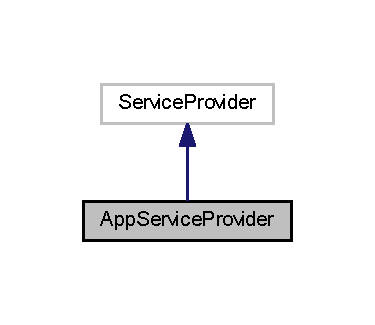
\includegraphics[width=180pt]{class_app_1_1_providers_1_1_app_service_provider__inherit__graph}
\end{center}
\end{figure}


Collaboration diagram for App\+Service\+Provider\+:
\nopagebreak
\begin{figure}[H]
\begin{center}
\leavevmode
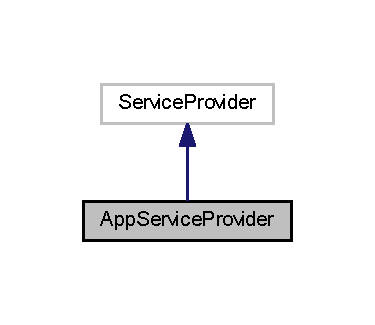
\includegraphics[width=180pt]{class_app_1_1_providers_1_1_app_service_provider__coll__graph}
\end{center}
\end{figure}
\subsection*{Public Member Functions}
\begin{DoxyCompactItemize}
\item 
\mbox{\hyperlink{class_app_1_1_providers_1_1_app_service_provider_acc294a6cc8e69743746820e3d15e3f78}{register}} ()
\end{DoxyCompactItemize}


\subsection{Member Function Documentation}
\mbox{\Hypertarget{class_app_1_1_providers_1_1_app_service_provider_acc294a6cc8e69743746820e3d15e3f78}\label{class_app_1_1_providers_1_1_app_service_provider_acc294a6cc8e69743746820e3d15e3f78}} 
\index{App\+::\+Providers\+::\+App\+Service\+Provider@{App\+::\+Providers\+::\+App\+Service\+Provider}!register@{register}}
\index{register@{register}!App\+::\+Providers\+::\+App\+Service\+Provider@{App\+::\+Providers\+::\+App\+Service\+Provider}}
\subsubsection{\texorpdfstring{register()}{register()}}
{\footnotesize\ttfamily register (\begin{DoxyParamCaption}{ }\end{DoxyParamCaption})}

Register any application services.

\begin{DoxyReturn}{Returns}
void 
\end{DoxyReturn}


The documentation for this class was generated from the following file\+:\begin{DoxyCompactItemize}
\item 
app/\+Providers/App\+Service\+Provider.\+php\end{DoxyCompactItemize}

\hypertarget{class_app_1_1_http_1_1_middleware_1_1_authenticate}{}\section{Authenticate Class Reference}
\label{class_app_1_1_http_1_1_middleware_1_1_authenticate}\index{Authenticate@{Authenticate}}
\subsection*{Public Member Functions}
\begin{DoxyCompactItemize}
\item 
\mbox{\hyperlink{class_app_1_1_http_1_1_middleware_1_1_authenticate_a4fc8a33bcaac7c3af3e9969dda3711ce}{\+\_\+\+\_\+construct}} (Auth \$auth)
\item 
\mbox{\hyperlink{class_app_1_1_http_1_1_middleware_1_1_authenticate_a9a62f11233fd9dce6393364e01b04001}{handle}} (\$request, Closure \$next, \$guard=null)
\end{DoxyCompactItemize}
\subsection*{Protected Attributes}
\begin{DoxyCompactItemize}
\item 
\mbox{\Hypertarget{class_app_1_1_http_1_1_middleware_1_1_authenticate_a20d7415a9c3391b32d7fe2136fce6e2c}\label{class_app_1_1_http_1_1_middleware_1_1_authenticate_a20d7415a9c3391b32d7fe2136fce6e2c}} 
{\bfseries \$auth}
\end{DoxyCompactItemize}


\subsection{Constructor \& Destructor Documentation}
\mbox{\Hypertarget{class_app_1_1_http_1_1_middleware_1_1_authenticate_a4fc8a33bcaac7c3af3e9969dda3711ce}\label{class_app_1_1_http_1_1_middleware_1_1_authenticate_a4fc8a33bcaac7c3af3e9969dda3711ce}} 
\index{App\+::\+Http\+::\+Middleware\+::\+Authenticate@{App\+::\+Http\+::\+Middleware\+::\+Authenticate}!\+\_\+\+\_\+construct@{\+\_\+\+\_\+construct}}
\index{\+\_\+\+\_\+construct@{\+\_\+\+\_\+construct}!App\+::\+Http\+::\+Middleware\+::\+Authenticate@{App\+::\+Http\+::\+Middleware\+::\+Authenticate}}
\subsubsection{\texorpdfstring{\+\_\+\+\_\+construct()}{\_\_construct()}}
{\footnotesize\ttfamily \+\_\+\+\_\+construct (\begin{DoxyParamCaption}\item[{Auth}]{\$auth }\end{DoxyParamCaption})}

Create a new middleware instance.


\begin{DoxyParams}[1]{Parameters}
\textbackslash{}\+Illuminate\textbackslash{}\+Contracts\textbackslash{}\+Auth\textbackslash{}\+Factory & {\em \$auth} & \\
\hline
\end{DoxyParams}
\begin{DoxyReturn}{Returns}
void 
\end{DoxyReturn}


\subsection{Member Function Documentation}
\mbox{\Hypertarget{class_app_1_1_http_1_1_middleware_1_1_authenticate_a9a62f11233fd9dce6393364e01b04001}\label{class_app_1_1_http_1_1_middleware_1_1_authenticate_a9a62f11233fd9dce6393364e01b04001}} 
\index{App\+::\+Http\+::\+Middleware\+::\+Authenticate@{App\+::\+Http\+::\+Middleware\+::\+Authenticate}!handle@{handle}}
\index{handle@{handle}!App\+::\+Http\+::\+Middleware\+::\+Authenticate@{App\+::\+Http\+::\+Middleware\+::\+Authenticate}}
\subsubsection{\texorpdfstring{handle()}{handle()}}
{\footnotesize\ttfamily handle (\begin{DoxyParamCaption}\item[{}]{\$request,  }\item[{Closure}]{\$next,  }\item[{}]{\$guard = {\ttfamily null} }\end{DoxyParamCaption})}

Handle an incoming request.


\begin{DoxyParams}[1]{Parameters}
\textbackslash{}\+Illuminate\textbackslash{}\+Http\textbackslash{}\+Request & {\em \$request} & \\
\hline
\textbackslash{}\+Closure & {\em \$next} & \\
\hline
string | null & {\em \$guard} & \\
\hline
\end{DoxyParams}
\begin{DoxyReturn}{Returns}
mixed 
\end{DoxyReturn}


The documentation for this class was generated from the following file\+:\begin{DoxyCompactItemize}
\item 
app/\+Http/\+Middleware/Authenticate.\+php\end{DoxyCompactItemize}

\hypertarget{class_app_1_1_providers_1_1_auth_service_provider}{}\section{Auth\+Service\+Provider Class Reference}
\label{class_app_1_1_providers_1_1_auth_service_provider}\index{Auth\+Service\+Provider@{Auth\+Service\+Provider}}


Inheritance diagram for Auth\+Service\+Provider\+:
\nopagebreak
\begin{figure}[H]
\begin{center}
\leavevmode
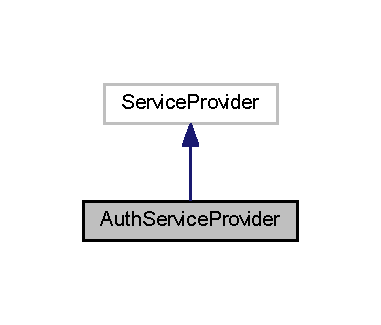
\includegraphics[width=183pt]{class_app_1_1_providers_1_1_auth_service_provider__inherit__graph}
\end{center}
\end{figure}


Collaboration diagram for Auth\+Service\+Provider\+:
\nopagebreak
\begin{figure}[H]
\begin{center}
\leavevmode
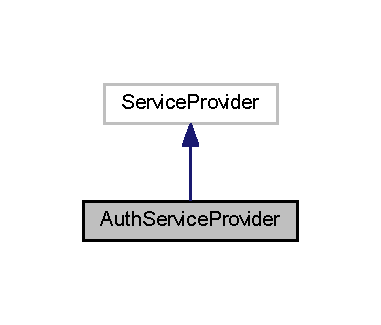
\includegraphics[width=183pt]{class_app_1_1_providers_1_1_auth_service_provider__coll__graph}
\end{center}
\end{figure}
\subsection*{Public Member Functions}
\begin{DoxyCompactItemize}
\item 
\mbox{\hyperlink{class_app_1_1_providers_1_1_auth_service_provider_acc294a6cc8e69743746820e3d15e3f78}{register}} ()
\item 
\mbox{\hyperlink{class_app_1_1_providers_1_1_auth_service_provider_a8814ea4b5beba763c570b4818980814e}{boot}} ()
\end{DoxyCompactItemize}


\subsection{Member Function Documentation}
\mbox{\Hypertarget{class_app_1_1_providers_1_1_auth_service_provider_a8814ea4b5beba763c570b4818980814e}\label{class_app_1_1_providers_1_1_auth_service_provider_a8814ea4b5beba763c570b4818980814e}} 
\index{App\+::\+Providers\+::\+Auth\+Service\+Provider@{App\+::\+Providers\+::\+Auth\+Service\+Provider}!boot@{boot}}
\index{boot@{boot}!App\+::\+Providers\+::\+Auth\+Service\+Provider@{App\+::\+Providers\+::\+Auth\+Service\+Provider}}
\subsubsection{\texorpdfstring{boot()}{boot()}}
{\footnotesize\ttfamily boot (\begin{DoxyParamCaption}{ }\end{DoxyParamCaption})}

Boot the authentication services for the application.

\begin{DoxyReturn}{Returns}
void 
\end{DoxyReturn}
\mbox{\Hypertarget{class_app_1_1_providers_1_1_auth_service_provider_acc294a6cc8e69743746820e3d15e3f78}\label{class_app_1_1_providers_1_1_auth_service_provider_acc294a6cc8e69743746820e3d15e3f78}} 
\index{App\+::\+Providers\+::\+Auth\+Service\+Provider@{App\+::\+Providers\+::\+Auth\+Service\+Provider}!register@{register}}
\index{register@{register}!App\+::\+Providers\+::\+Auth\+Service\+Provider@{App\+::\+Providers\+::\+Auth\+Service\+Provider}}
\subsubsection{\texorpdfstring{register()}{register()}}
{\footnotesize\ttfamily register (\begin{DoxyParamCaption}{ }\end{DoxyParamCaption})}

Register any application services.

\begin{DoxyReturn}{Returns}
void 
\end{DoxyReturn}


The documentation for this class was generated from the following file\+:\begin{DoxyCompactItemize}
\item 
app/\+Providers/Auth\+Service\+Provider.\+php\end{DoxyCompactItemize}

\hypertarget{class_app_1_1_models_1_1_card}{}\section{Card Class Reference}
\label{class_app_1_1_models_1_1_card}\index{Card@{Card}}


Inheritance diagram for Card\+:
\nopagebreak
\begin{figure}[H]
\begin{center}
\leavevmode
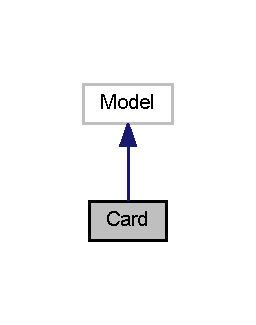
\includegraphics[width=123pt]{class_app_1_1_models_1_1_card__inherit__graph}
\end{center}
\end{figure}


Collaboration diagram for Card\+:
\nopagebreak
\begin{figure}[H]
\begin{center}
\leavevmode
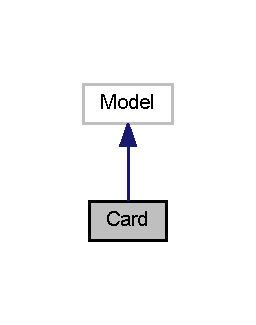
\includegraphics[width=123pt]{class_app_1_1_models_1_1_card__coll__graph}
\end{center}
\end{figure}
\subsection*{Protected Attributes}
\begin{DoxyCompactItemize}
\item 
\mbox{\Hypertarget{class_app_1_1_models_1_1_card_ae8876a14058f368335baccf35af4a22b}\label{class_app_1_1_models_1_1_card_ae8876a14058f368335baccf35af4a22b}} 
{\bfseries \$table} = \textquotesingle{}cards\textquotesingle{}
\item 
{\bfseries \$fillabe}
\end{DoxyCompactItemize}


\subsection{Detailed Description}
This model represents types of cards. Could be credit card, debit card, or just money!

Accepts name\+: string, status\+: tiny\+Integer. Status represents if the card is available at the moment. 

\subsection{Field Documentation}
\mbox{\Hypertarget{class_app_1_1_models_1_1_card_ac5c29ce22e45a54200f88204e498d290}\label{class_app_1_1_models_1_1_card_ac5c29ce22e45a54200f88204e498d290}} 
\index{App\+::\+Models\+::\+Card@{App\+::\+Models\+::\+Card}!\$fillabe@{\$fillabe}}
\index{\$fillabe@{\$fillabe}!App\+::\+Models\+::\+Card@{App\+::\+Models\+::\+Card}}
\subsubsection{\texorpdfstring{\$fillabe}{$fillabe}}
{\footnotesize\ttfamily \$fillabe\hspace{0.3cm}{\ttfamily [protected]}}

{\bfseries Initial value\+:}
\begin{DoxyCode}
= [
        \textcolor{stringliteral}{'name'},
        \textcolor{stringliteral}{'status'}
    ]
\end{DoxyCode}


The documentation for this class was generated from the following file\+:\begin{DoxyCompactItemize}
\item 
app/\+Models/Card.\+php\end{DoxyCompactItemize}

\hypertarget{class_app_1_1_http_1_1_controllers_1_1_card_controller}{}\section{Card\+Controller Class Reference}
\label{class_app_1_1_http_1_1_controllers_1_1_card_controller}\index{Card\+Controller@{Card\+Controller}}


Inheritance diagram for Card\+Controller\+:
\nopagebreak
\begin{figure}[H]
\begin{center}
\leavevmode
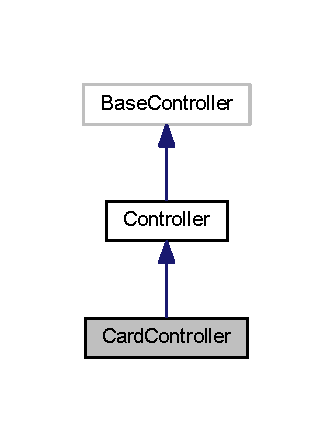
\includegraphics[width=160pt]{class_app_1_1_http_1_1_controllers_1_1_card_controller__inherit__graph}
\end{center}
\end{figure}


Collaboration diagram for Card\+Controller\+:
\nopagebreak
\begin{figure}[H]
\begin{center}
\leavevmode
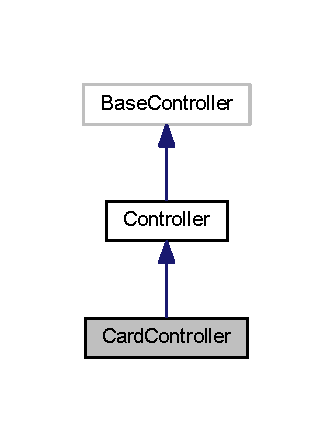
\includegraphics[width=160pt]{class_app_1_1_http_1_1_controllers_1_1_card_controller__coll__graph}
\end{center}
\end{figure}
\subsection*{Public Member Functions}
\begin{DoxyCompactItemize}
\item 
\mbox{\hyperlink{class_app_1_1_http_1_1_controllers_1_1_card_controller_a5b75ba6bc9debb999c0186a31978ec03}{\+\_\+\+\_\+construct}} (\$repository)
\item 
\mbox{\hyperlink{class_app_1_1_http_1_1_controllers_1_1_card_controller_a149eb92716c1084a935e04a8d95f7347}{index}} ()
\item 
\mbox{\hyperlink{class_app_1_1_http_1_1_controllers_1_1_card_controller_a4fa811c83f27da01b0d92bdb2a711a13}{create}} (\$request)
\item 
\mbox{\hyperlink{class_app_1_1_http_1_1_controllers_1_1_card_controller_ab7b27a90191560dcef32126b0945db0d}{update}} (\$request)
\item 
\mbox{\hyperlink{class_app_1_1_http_1_1_controllers_1_1_card_controller_a126a3799c44d72393ca4732081306dfd}{delete}} (\$request)
\end{DoxyCompactItemize}


\subsection{Detailed Description}
\mbox{\hyperlink{class_app_1_1_http_1_1_controllers_1_1_controller}{Controller}} for the cards. 

\subsection{Constructor \& Destructor Documentation}
\mbox{\Hypertarget{class_app_1_1_http_1_1_controllers_1_1_card_controller_a5b75ba6bc9debb999c0186a31978ec03}\label{class_app_1_1_http_1_1_controllers_1_1_card_controller_a5b75ba6bc9debb999c0186a31978ec03}} 
\index{App\+::\+Http\+::\+Controllers\+::\+Card\+Controller@{App\+::\+Http\+::\+Controllers\+::\+Card\+Controller}!\+\_\+\+\_\+construct@{\+\_\+\+\_\+construct}}
\index{\+\_\+\+\_\+construct@{\+\_\+\+\_\+construct}!App\+::\+Http\+::\+Controllers\+::\+Card\+Controller@{App\+::\+Http\+::\+Controllers\+::\+Card\+Controller}}
\subsubsection{\texorpdfstring{\+\_\+\+\_\+construct()}{\_\_construct()}}
{\footnotesize\ttfamily \+\_\+\+\_\+construct (\begin{DoxyParamCaption}\item[{}]{\$repository }\end{DoxyParamCaption})}

Using dependency injection to get the repository connected to the A\+PI in the app\+\_\+providers.


\begin{DoxyParams}[1]{Parameters}
interface & {\em \$repository} & \\
\hline
\end{DoxyParams}


\subsection{Member Function Documentation}
\mbox{\Hypertarget{class_app_1_1_http_1_1_controllers_1_1_card_controller_a4fa811c83f27da01b0d92bdb2a711a13}\label{class_app_1_1_http_1_1_controllers_1_1_card_controller_a4fa811c83f27da01b0d92bdb2a711a13}} 
\index{App\+::\+Http\+::\+Controllers\+::\+Card\+Controller@{App\+::\+Http\+::\+Controllers\+::\+Card\+Controller}!create@{create}}
\index{create@{create}!App\+::\+Http\+::\+Controllers\+::\+Card\+Controller@{App\+::\+Http\+::\+Controllers\+::\+Card\+Controller}}
\subsubsection{\texorpdfstring{create()}{create()}}
{\footnotesize\ttfamily create (\begin{DoxyParamCaption}\item[{}]{\$request }\end{DoxyParamCaption})}

Store a new card.

\begin{DoxyReturn}{Returns}
boolean 
\end{DoxyReturn}
\mbox{\Hypertarget{class_app_1_1_http_1_1_controllers_1_1_card_controller_a126a3799c44d72393ca4732081306dfd}\label{class_app_1_1_http_1_1_controllers_1_1_card_controller_a126a3799c44d72393ca4732081306dfd}} 
\index{App\+::\+Http\+::\+Controllers\+::\+Card\+Controller@{App\+::\+Http\+::\+Controllers\+::\+Card\+Controller}!delete@{delete}}
\index{delete@{delete}!App\+::\+Http\+::\+Controllers\+::\+Card\+Controller@{App\+::\+Http\+::\+Controllers\+::\+Card\+Controller}}
\subsubsection{\texorpdfstring{delete()}{delete()}}
{\footnotesize\ttfamily delete (\begin{DoxyParamCaption}\item[{}]{\$request }\end{DoxyParamCaption})}

Delete a card.

\begin{DoxyReturn}{Returns}
boolean 
\end{DoxyReturn}
\mbox{\Hypertarget{class_app_1_1_http_1_1_controllers_1_1_card_controller_a149eb92716c1084a935e04a8d95f7347}\label{class_app_1_1_http_1_1_controllers_1_1_card_controller_a149eb92716c1084a935e04a8d95f7347}} 
\index{App\+::\+Http\+::\+Controllers\+::\+Card\+Controller@{App\+::\+Http\+::\+Controllers\+::\+Card\+Controller}!index@{index}}
\index{index@{index}!App\+::\+Http\+::\+Controllers\+::\+Card\+Controller@{App\+::\+Http\+::\+Controllers\+::\+Card\+Controller}}
\subsubsection{\texorpdfstring{index()}{index()}}
{\footnotesize\ttfamily index (\begin{DoxyParamCaption}{ }\end{DoxyParamCaption})}

Returns all the cards.

\begin{DoxyReturn}{Returns}
array 
\end{DoxyReturn}
\mbox{\Hypertarget{class_app_1_1_http_1_1_controllers_1_1_card_controller_ab7b27a90191560dcef32126b0945db0d}\label{class_app_1_1_http_1_1_controllers_1_1_card_controller_ab7b27a90191560dcef32126b0945db0d}} 
\index{App\+::\+Http\+::\+Controllers\+::\+Card\+Controller@{App\+::\+Http\+::\+Controllers\+::\+Card\+Controller}!update@{update}}
\index{update@{update}!App\+::\+Http\+::\+Controllers\+::\+Card\+Controller@{App\+::\+Http\+::\+Controllers\+::\+Card\+Controller}}
\subsubsection{\texorpdfstring{update()}{update()}}
{\footnotesize\ttfamily update (\begin{DoxyParamCaption}\item[{}]{\$request }\end{DoxyParamCaption})}

Update a card.

\begin{DoxyReturn}{Returns}
boolean 
\end{DoxyReturn}


The documentation for this class was generated from the following file\+:\begin{DoxyCompactItemize}
\item 
app/\+Http/\+Controllers/Card\+Controller.\+php\end{DoxyCompactItemize}

\hypertarget{class_app_1_1_models_1_1_product_1_1_category}{}\section{Category Class Reference}
\label{class_app_1_1_models_1_1_product_1_1_category}\index{Category@{Category}}


Inheritance diagram for Category\+:
\nopagebreak
\begin{figure}[H]
\begin{center}
\leavevmode
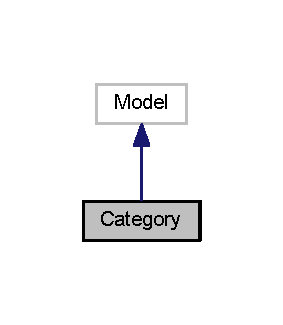
\includegraphics[width=136pt]{class_app_1_1_models_1_1_product_1_1_category__inherit__graph}
\end{center}
\end{figure}


Collaboration diagram for Category\+:
\nopagebreak
\begin{figure}[H]
\begin{center}
\leavevmode
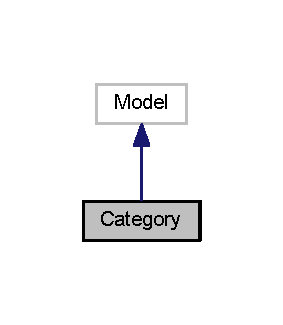
\includegraphics[width=136pt]{class_app_1_1_models_1_1_product_1_1_category__coll__graph}
\end{center}
\end{figure}
\subsection*{Protected Attributes}
\begin{DoxyCompactItemize}
\item 
\mbox{\Hypertarget{class_app_1_1_models_1_1_product_1_1_category_ae8876a14058f368335baccf35af4a22b}\label{class_app_1_1_models_1_1_product_1_1_category_ae8876a14058f368335baccf35af4a22b}} 
{\bfseries \$table} = \textquotesingle{}product\+\_\+categories\textquotesingle{}
\item 
{\bfseries \$fillabe}
\end{DoxyCompactItemize}


\subsection{Detailed Description}
Represents the category of a \mbox{\hyperlink{class_app_1_1_models_1_1_product_1_1_product}{Product}}. Could be food or drink.

Accepts name\+: string 

\subsection{Field Documentation}
\mbox{\Hypertarget{class_app_1_1_models_1_1_product_1_1_category_ac5c29ce22e45a54200f88204e498d290}\label{class_app_1_1_models_1_1_product_1_1_category_ac5c29ce22e45a54200f88204e498d290}} 
\index{App\+::\+Models\+::\+Product\+::\+Category@{App\+::\+Models\+::\+Product\+::\+Category}!\$fillabe@{\$fillabe}}
\index{\$fillabe@{\$fillabe}!App\+::\+Models\+::\+Product\+::\+Category@{App\+::\+Models\+::\+Product\+::\+Category}}
\subsubsection{\texorpdfstring{\$fillabe}{$fillabe}}
{\footnotesize\ttfamily \$fillabe\hspace{0.3cm}{\ttfamily [protected]}}

{\bfseries Initial value\+:}
\begin{DoxyCode}
= [
        \textcolor{stringliteral}{'name'},
    ]
\end{DoxyCode}


The documentation for this class was generated from the following file\+:\begin{DoxyCompactItemize}
\item 
app/\+Models/\+Product/Category.\+php\end{DoxyCompactItemize}

\hypertarget{class_app_1_1_http_1_1_controllers_1_1_product_1_1_category_controller}{}\section{Category\+Controller Class Reference}
\label{class_app_1_1_http_1_1_controllers_1_1_product_1_1_category_controller}\index{Category\+Controller@{Category\+Controller}}


Inheritance diagram for Category\+Controller\+:
\nopagebreak
\begin{figure}[H]
\begin{center}
\leavevmode
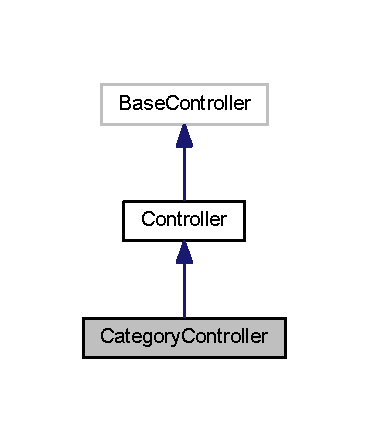
\includegraphics[width=177pt]{class_app_1_1_http_1_1_controllers_1_1_product_1_1_category_controller__inherit__graph}
\end{center}
\end{figure}


Collaboration diagram for Category\+Controller\+:
\nopagebreak
\begin{figure}[H]
\begin{center}
\leavevmode
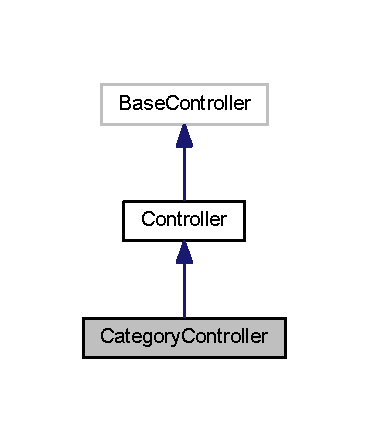
\includegraphics[width=177pt]{class_app_1_1_http_1_1_controllers_1_1_product_1_1_category_controller__coll__graph}
\end{center}
\end{figure}
\subsection*{Public Member Functions}
\begin{DoxyCompactItemize}
\item 
\mbox{\hyperlink{class_app_1_1_http_1_1_controllers_1_1_product_1_1_category_controller_a5b75ba6bc9debb999c0186a31978ec03}{\+\_\+\+\_\+construct}} (\$repository)
\item 
\mbox{\hyperlink{class_app_1_1_http_1_1_controllers_1_1_product_1_1_category_controller_af9d14e4ae6227970ad603987781573ca}{all}} ()
\item 
\mbox{\hyperlink{class_app_1_1_http_1_1_controllers_1_1_product_1_1_category_controller_a50e3bfb586b2f42932a6a93f3fbb0828}{get}} (\$id)
\item 
\mbox{\hyperlink{class_app_1_1_http_1_1_controllers_1_1_product_1_1_category_controller_a4fa811c83f27da01b0d92bdb2a711a13}{create}} (\$request)
\item 
\mbox{\hyperlink{class_app_1_1_http_1_1_controllers_1_1_product_1_1_category_controller_ab7b27a90191560dcef32126b0945db0d}{update}} (\$request)
\item 
\mbox{\hyperlink{class_app_1_1_http_1_1_controllers_1_1_product_1_1_category_controller_a126a3799c44d72393ca4732081306dfd}{delete}} (\$request)
\end{DoxyCompactItemize}


\subsection{Detailed Description}
\mbox{\hyperlink{class_app_1_1_http_1_1_controllers_1_1_controller}{Controller}} for the product categories. 

\subsection{Constructor \& Destructor Documentation}
\mbox{\Hypertarget{class_app_1_1_http_1_1_controllers_1_1_product_1_1_category_controller_a5b75ba6bc9debb999c0186a31978ec03}\label{class_app_1_1_http_1_1_controllers_1_1_product_1_1_category_controller_a5b75ba6bc9debb999c0186a31978ec03}} 
\index{App\+::\+Http\+::\+Controllers\+::\+Product\+::\+Category\+Controller@{App\+::\+Http\+::\+Controllers\+::\+Product\+::\+Category\+Controller}!\+\_\+\+\_\+construct@{\+\_\+\+\_\+construct}}
\index{\+\_\+\+\_\+construct@{\+\_\+\+\_\+construct}!App\+::\+Http\+::\+Controllers\+::\+Product\+::\+Category\+Controller@{App\+::\+Http\+::\+Controllers\+::\+Product\+::\+Category\+Controller}}
\subsubsection{\texorpdfstring{\+\_\+\+\_\+construct()}{\_\_construct()}}
{\footnotesize\ttfamily \+\_\+\+\_\+construct (\begin{DoxyParamCaption}\item[{}]{\$repository }\end{DoxyParamCaption})}

Using dependency injection to get the repository connected to the A\+PI in the app\+\_\+providers.


\begin{DoxyParams}[1]{Parameters}
interface & {\em \$repository} & \\
\hline
\end{DoxyParams}


\subsection{Member Function Documentation}
\mbox{\Hypertarget{class_app_1_1_http_1_1_controllers_1_1_product_1_1_category_controller_af9d14e4ae6227970ad603987781573ca}\label{class_app_1_1_http_1_1_controllers_1_1_product_1_1_category_controller_af9d14e4ae6227970ad603987781573ca}} 
\index{App\+::\+Http\+::\+Controllers\+::\+Product\+::\+Category\+Controller@{App\+::\+Http\+::\+Controllers\+::\+Product\+::\+Category\+Controller}!all@{all}}
\index{all@{all}!App\+::\+Http\+::\+Controllers\+::\+Product\+::\+Category\+Controller@{App\+::\+Http\+::\+Controllers\+::\+Product\+::\+Category\+Controller}}
\subsubsection{\texorpdfstring{all()}{all()}}
{\footnotesize\ttfamily all (\begin{DoxyParamCaption}{ }\end{DoxyParamCaption})}

Returns an array of Category objects.

\begin{DoxyReturn}{Returns}
array 
\end{DoxyReturn}
\mbox{\Hypertarget{class_app_1_1_http_1_1_controllers_1_1_product_1_1_category_controller_a4fa811c83f27da01b0d92bdb2a711a13}\label{class_app_1_1_http_1_1_controllers_1_1_product_1_1_category_controller_a4fa811c83f27da01b0d92bdb2a711a13}} 
\index{App\+::\+Http\+::\+Controllers\+::\+Product\+::\+Category\+Controller@{App\+::\+Http\+::\+Controllers\+::\+Product\+::\+Category\+Controller}!create@{create}}
\index{create@{create}!App\+::\+Http\+::\+Controllers\+::\+Product\+::\+Category\+Controller@{App\+::\+Http\+::\+Controllers\+::\+Product\+::\+Category\+Controller}}
\subsubsection{\texorpdfstring{create()}{create()}}
{\footnotesize\ttfamily create (\begin{DoxyParamCaption}\item[{}]{\$request }\end{DoxyParamCaption})}

Store a new category.

\begin{DoxyReturn}{Returns}
boolean 
\end{DoxyReturn}
\mbox{\Hypertarget{class_app_1_1_http_1_1_controllers_1_1_product_1_1_category_controller_a126a3799c44d72393ca4732081306dfd}\label{class_app_1_1_http_1_1_controllers_1_1_product_1_1_category_controller_a126a3799c44d72393ca4732081306dfd}} 
\index{App\+::\+Http\+::\+Controllers\+::\+Product\+::\+Category\+Controller@{App\+::\+Http\+::\+Controllers\+::\+Product\+::\+Category\+Controller}!delete@{delete}}
\index{delete@{delete}!App\+::\+Http\+::\+Controllers\+::\+Product\+::\+Category\+Controller@{App\+::\+Http\+::\+Controllers\+::\+Product\+::\+Category\+Controller}}
\subsubsection{\texorpdfstring{delete()}{delete()}}
{\footnotesize\ttfamily delete (\begin{DoxyParamCaption}\item[{}]{\$request }\end{DoxyParamCaption})}

Delete a category.

\begin{DoxyReturn}{Returns}
boolean 
\end{DoxyReturn}
\mbox{\Hypertarget{class_app_1_1_http_1_1_controllers_1_1_product_1_1_category_controller_a50e3bfb586b2f42932a6a93f3fbb0828}\label{class_app_1_1_http_1_1_controllers_1_1_product_1_1_category_controller_a50e3bfb586b2f42932a6a93f3fbb0828}} 
\index{App\+::\+Http\+::\+Controllers\+::\+Product\+::\+Category\+Controller@{App\+::\+Http\+::\+Controllers\+::\+Product\+::\+Category\+Controller}!get@{get}}
\index{get@{get}!App\+::\+Http\+::\+Controllers\+::\+Product\+::\+Category\+Controller@{App\+::\+Http\+::\+Controllers\+::\+Product\+::\+Category\+Controller}}
\subsubsection{\texorpdfstring{get()}{get()}}
{\footnotesize\ttfamily get (\begin{DoxyParamCaption}\item[{}]{\$id }\end{DoxyParamCaption})}

Returns an Category Object with the provided id.

\begin{DoxyReturn}{Returns}
object 
\end{DoxyReturn}
\mbox{\Hypertarget{class_app_1_1_http_1_1_controllers_1_1_product_1_1_category_controller_ab7b27a90191560dcef32126b0945db0d}\label{class_app_1_1_http_1_1_controllers_1_1_product_1_1_category_controller_ab7b27a90191560dcef32126b0945db0d}} 
\index{App\+::\+Http\+::\+Controllers\+::\+Product\+::\+Category\+Controller@{App\+::\+Http\+::\+Controllers\+::\+Product\+::\+Category\+Controller}!update@{update}}
\index{update@{update}!App\+::\+Http\+::\+Controllers\+::\+Product\+::\+Category\+Controller@{App\+::\+Http\+::\+Controllers\+::\+Product\+::\+Category\+Controller}}
\subsubsection{\texorpdfstring{update()}{update()}}
{\footnotesize\ttfamily update (\begin{DoxyParamCaption}\item[{}]{\$request }\end{DoxyParamCaption})}

Update a category.

\begin{DoxyReturn}{Returns}
boolean 
\end{DoxyReturn}


The documentation for this class was generated from the following file\+:\begin{DoxyCompactItemize}
\item 
app/\+Http/\+Controllers/\+Product/Category\+Controller.\+php\end{DoxyCompactItemize}

\hypertarget{interface_app_1_1_repositories_1_1_product_1_1_category_repository_interface}{}\section{Category\+Repository\+Interface Interface Reference}
\label{interface_app_1_1_repositories_1_1_product_1_1_category_repository_interface}\index{Category\+Repository\+Interface@{Category\+Repository\+Interface}}
\subsection*{Public Member Functions}
\begin{DoxyCompactItemize}
\item 
\mbox{\hyperlink{interface_app_1_1_repositories_1_1_product_1_1_category_repository_interface_af9d14e4ae6227970ad603987781573ca}{all}} ()
\item 
\mbox{\hyperlink{interface_app_1_1_repositories_1_1_product_1_1_category_repository_interface_a50e3bfb586b2f42932a6a93f3fbb0828}{get}} (\$id)
\item 
\mbox{\hyperlink{interface_app_1_1_repositories_1_1_product_1_1_category_repository_interface_a4fa811c83f27da01b0d92bdb2a711a13}{create}} (\$request)
\item 
\mbox{\hyperlink{interface_app_1_1_repositories_1_1_product_1_1_category_repository_interface_a2aedea52c52e54ba3c4c9f60423e7ef1}{udpate}} (\$request)
\item 
\mbox{\hyperlink{interface_app_1_1_repositories_1_1_product_1_1_category_repository_interface_a126a3799c44d72393ca4732081306dfd}{delete}} (\$request)
\end{DoxyCompactItemize}


\subsection{Detailed Description}
Interface for the Category\+Repository 

\subsection{Member Function Documentation}
\mbox{\Hypertarget{interface_app_1_1_repositories_1_1_product_1_1_category_repository_interface_af9d14e4ae6227970ad603987781573ca}\label{interface_app_1_1_repositories_1_1_product_1_1_category_repository_interface_af9d14e4ae6227970ad603987781573ca}} 
\index{App\+::\+Repositories\+::\+Product\+::\+Category\+Repository\+Interface@{App\+::\+Repositories\+::\+Product\+::\+Category\+Repository\+Interface}!all@{all}}
\index{all@{all}!App\+::\+Repositories\+::\+Product\+::\+Category\+Repository\+Interface@{App\+::\+Repositories\+::\+Product\+::\+Category\+Repository\+Interface}}
\subsubsection{\texorpdfstring{all()}{all()}}
{\footnotesize\ttfamily all (\begin{DoxyParamCaption}{ }\end{DoxyParamCaption})}

Returns an array of Category objects.

\begin{DoxyReturn}{Returns}
array 
\end{DoxyReturn}
\mbox{\Hypertarget{interface_app_1_1_repositories_1_1_product_1_1_category_repository_interface_a4fa811c83f27da01b0d92bdb2a711a13}\label{interface_app_1_1_repositories_1_1_product_1_1_category_repository_interface_a4fa811c83f27da01b0d92bdb2a711a13}} 
\index{App\+::\+Repositories\+::\+Product\+::\+Category\+Repository\+Interface@{App\+::\+Repositories\+::\+Product\+::\+Category\+Repository\+Interface}!create@{create}}
\index{create@{create}!App\+::\+Repositories\+::\+Product\+::\+Category\+Repository\+Interface@{App\+::\+Repositories\+::\+Product\+::\+Category\+Repository\+Interface}}
\subsubsection{\texorpdfstring{create()}{create()}}
{\footnotesize\ttfamily create (\begin{DoxyParamCaption}\item[{}]{\$request }\end{DoxyParamCaption})}

Returns a boolean reflecting the creation status.

\begin{DoxyReturn}{Returns}
boolean 
\end{DoxyReturn}
\mbox{\Hypertarget{interface_app_1_1_repositories_1_1_product_1_1_category_repository_interface_a126a3799c44d72393ca4732081306dfd}\label{interface_app_1_1_repositories_1_1_product_1_1_category_repository_interface_a126a3799c44d72393ca4732081306dfd}} 
\index{App\+::\+Repositories\+::\+Product\+::\+Category\+Repository\+Interface@{App\+::\+Repositories\+::\+Product\+::\+Category\+Repository\+Interface}!delete@{delete}}
\index{delete@{delete}!App\+::\+Repositories\+::\+Product\+::\+Category\+Repository\+Interface@{App\+::\+Repositories\+::\+Product\+::\+Category\+Repository\+Interface}}
\subsubsection{\texorpdfstring{delete()}{delete()}}
{\footnotesize\ttfamily delete (\begin{DoxyParamCaption}\item[{}]{\$request }\end{DoxyParamCaption})}

Returns a boolean reflecting the deletion status.

\begin{DoxyReturn}{Returns}
boolean 
\end{DoxyReturn}
\mbox{\Hypertarget{interface_app_1_1_repositories_1_1_product_1_1_category_repository_interface_a50e3bfb586b2f42932a6a93f3fbb0828}\label{interface_app_1_1_repositories_1_1_product_1_1_category_repository_interface_a50e3bfb586b2f42932a6a93f3fbb0828}} 
\index{App\+::\+Repositories\+::\+Product\+::\+Category\+Repository\+Interface@{App\+::\+Repositories\+::\+Product\+::\+Category\+Repository\+Interface}!get@{get}}
\index{get@{get}!App\+::\+Repositories\+::\+Product\+::\+Category\+Repository\+Interface@{App\+::\+Repositories\+::\+Product\+::\+Category\+Repository\+Interface}}
\subsubsection{\texorpdfstring{get()}{get()}}
{\footnotesize\ttfamily get (\begin{DoxyParamCaption}\item[{}]{\$id }\end{DoxyParamCaption})}

Returns an Category Object with the provided id.

\begin{DoxyReturn}{Returns}
object 
\end{DoxyReturn}
\mbox{\Hypertarget{interface_app_1_1_repositories_1_1_product_1_1_category_repository_interface_a2aedea52c52e54ba3c4c9f60423e7ef1}\label{interface_app_1_1_repositories_1_1_product_1_1_category_repository_interface_a2aedea52c52e54ba3c4c9f60423e7ef1}} 
\index{App\+::\+Repositories\+::\+Product\+::\+Category\+Repository\+Interface@{App\+::\+Repositories\+::\+Product\+::\+Category\+Repository\+Interface}!udpate@{udpate}}
\index{udpate@{udpate}!App\+::\+Repositories\+::\+Product\+::\+Category\+Repository\+Interface@{App\+::\+Repositories\+::\+Product\+::\+Category\+Repository\+Interface}}
\subsubsection{\texorpdfstring{udpate()}{udpate()}}
{\footnotesize\ttfamily udpate (\begin{DoxyParamCaption}\item[{}]{\$request }\end{DoxyParamCaption})}

Returns a boolean reflecting the update status.

\begin{DoxyReturn}{Returns}
boolean 
\end{DoxyReturn}


The documentation for this interface was generated from the following file\+:\begin{DoxyCompactItemize}
\item 
app/\+Repositories/\+Product/Category\+Repository\+Interface.\+php\end{DoxyCompactItemize}

\hypertarget{class_app_1_1_http_1_1_controllers_1_1_controller}{}\section{Controller Class Reference}
\label{class_app_1_1_http_1_1_controllers_1_1_controller}\index{Controller@{Controller}}


Inheritance diagram for Controller\+:
\nopagebreak
\begin{figure}[H]
\begin{center}
\leavevmode
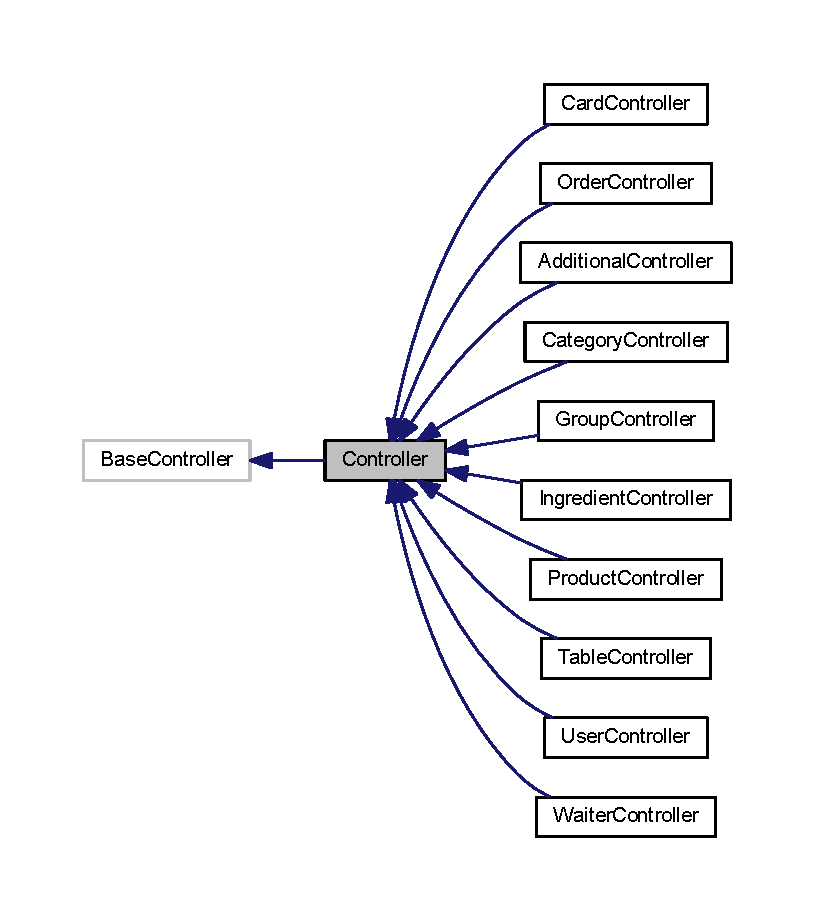
\includegraphics[width=350pt]{class_app_1_1_http_1_1_controllers_1_1_controller__inherit__graph}
\end{center}
\end{figure}


Collaboration diagram for Controller\+:
\nopagebreak
\begin{figure}[H]
\begin{center}
\leavevmode
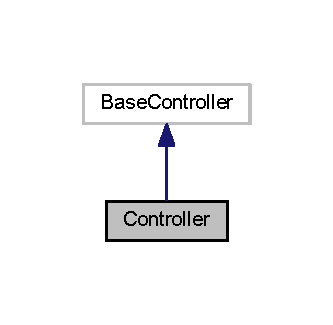
\includegraphics[width=160pt]{class_app_1_1_http_1_1_controllers_1_1_controller__coll__graph}
\end{center}
\end{figure}


The documentation for this class was generated from the following file\+:\begin{DoxyCompactItemize}
\item 
app/\+Http/\+Controllers/Controller.\+php\end{DoxyCompactItemize}

\hypertarget{class_app_1_1_providers_1_1_event_service_provider}{}\section{Event\+Service\+Provider Class Reference}
\label{class_app_1_1_providers_1_1_event_service_provider}\index{Event\+Service\+Provider@{Event\+Service\+Provider}}


Inheritance diagram for Event\+Service\+Provider\+:
\nopagebreak
\begin{figure}[H]
\begin{center}
\leavevmode
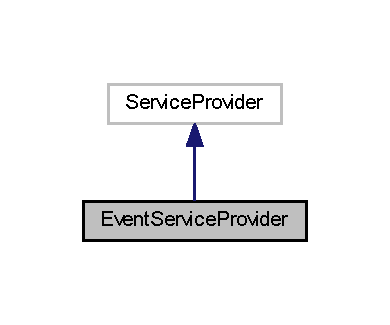
\includegraphics[width=187pt]{class_app_1_1_providers_1_1_event_service_provider__inherit__graph}
\end{center}
\end{figure}


Collaboration diagram for Event\+Service\+Provider\+:
\nopagebreak
\begin{figure}[H]
\begin{center}
\leavevmode
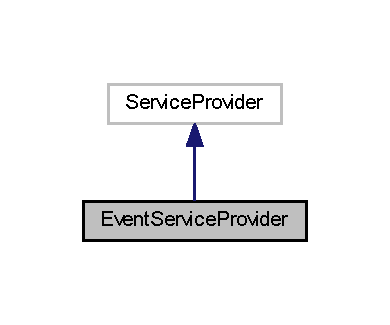
\includegraphics[width=187pt]{class_app_1_1_providers_1_1_event_service_provider__coll__graph}
\end{center}
\end{figure}
\subsection*{Protected Attributes}
\begin{DoxyCompactItemize}
\item 
{\bfseries \$listen}
\end{DoxyCompactItemize}


\subsection{Field Documentation}
\mbox{\Hypertarget{class_app_1_1_providers_1_1_event_service_provider_abdfd4689e0597f0b6c63b970c101e810}\label{class_app_1_1_providers_1_1_event_service_provider_abdfd4689e0597f0b6c63b970c101e810}} 
\index{App\+::\+Providers\+::\+Event\+Service\+Provider@{App\+::\+Providers\+::\+Event\+Service\+Provider}!\$listen@{\$listen}}
\index{\$listen@{\$listen}!App\+::\+Providers\+::\+Event\+Service\+Provider@{App\+::\+Providers\+::\+Event\+Service\+Provider}}
\subsubsection{\texorpdfstring{\$listen}{$listen}}
{\footnotesize\ttfamily \$listen\hspace{0.3cm}{\ttfamily [protected]}}

{\bfseries Initial value\+:}
\begin{DoxyCode}
= [
        \textcolor{stringliteral}{'App\(\backslash\)Events\(\backslash\)ExampleEvent'} => [
            \textcolor{stringliteral}{'App\(\backslash\)Listeners\(\backslash\)ExampleListener'},
        ]
\end{DoxyCode}


The documentation for this class was generated from the following file\+:\begin{DoxyCompactItemize}
\item 
app/\+Providers/Event\+Service\+Provider.\+php\end{DoxyCompactItemize}

\hypertarget{class_app_1_1_http_1_1_middleware_1_1_example_middleware}{}\section{Example\+Middleware Class Reference}
\label{class_app_1_1_http_1_1_middleware_1_1_example_middleware}\index{Example\+Middleware@{Example\+Middleware}}
\subsection*{Public Member Functions}
\begin{DoxyCompactItemize}
\item 
\mbox{\hyperlink{class_app_1_1_http_1_1_middleware_1_1_example_middleware_acef7660b2651389395d139e8af42d670}{handle}} (\$request, Closure \$next)
\end{DoxyCompactItemize}


\subsection{Member Function Documentation}
\mbox{\Hypertarget{class_app_1_1_http_1_1_middleware_1_1_example_middleware_acef7660b2651389395d139e8af42d670}\label{class_app_1_1_http_1_1_middleware_1_1_example_middleware_acef7660b2651389395d139e8af42d670}} 
\index{App\+::\+Http\+::\+Middleware\+::\+Example\+Middleware@{App\+::\+Http\+::\+Middleware\+::\+Example\+Middleware}!handle@{handle}}
\index{handle@{handle}!App\+::\+Http\+::\+Middleware\+::\+Example\+Middleware@{App\+::\+Http\+::\+Middleware\+::\+Example\+Middleware}}
\subsubsection{\texorpdfstring{handle()}{handle()}}
{\footnotesize\ttfamily handle (\begin{DoxyParamCaption}\item[{}]{\$request,  }\item[{Closure}]{\$next }\end{DoxyParamCaption})}

Handle an incoming request.


\begin{DoxyParams}[1]{Parameters}
\textbackslash{}\+Illuminate\textbackslash{}\+Http\textbackslash{}\+Request & {\em \$request} & \\
\hline
\textbackslash{}\+Closure & {\em \$next} & \\
\hline
\end{DoxyParams}
\begin{DoxyReturn}{Returns}
mixed 
\end{DoxyReturn}


The documentation for this class was generated from the following file\+:\begin{DoxyCompactItemize}
\item 
app/\+Http/\+Middleware/Example\+Middleware.\+php\end{DoxyCompactItemize}

\hypertarget{class_app_1_1_models_1_1_product_1_1_group}{}\section{Group Class Reference}
\label{class_app_1_1_models_1_1_product_1_1_group}\index{Group@{Group}}


Inheritance diagram for Group\+:
\nopagebreak
\begin{figure}[H]
\begin{center}
\leavevmode
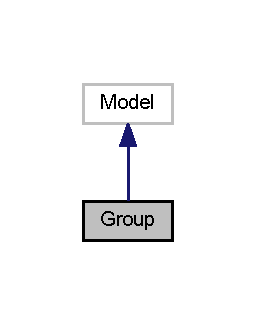
\includegraphics[width=123pt]{class_app_1_1_models_1_1_product_1_1_group__inherit__graph}
\end{center}
\end{figure}


Collaboration diagram for Group\+:
\nopagebreak
\begin{figure}[H]
\begin{center}
\leavevmode
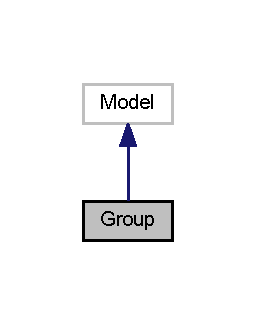
\includegraphics[width=123pt]{class_app_1_1_models_1_1_product_1_1_group__coll__graph}
\end{center}
\end{figure}
\subsection*{Protected Attributes}
\begin{DoxyCompactItemize}
\item 
\mbox{\Hypertarget{class_app_1_1_models_1_1_product_1_1_group_ae8876a14058f368335baccf35af4a22b}\label{class_app_1_1_models_1_1_product_1_1_group_ae8876a14058f368335baccf35af4a22b}} 
{\bfseries \$table} = \textquotesingle{}product\+\_\+groups\textquotesingle{}
\item 
{\bfseries \$fillabe}
\end{DoxyCompactItemize}


\subsection{Detailed Description}
Represents the group a product is connected to. Could be burger, quick plates, beers, wines, waters, vegetarians

Accepts name\+: string. 

\subsection{Field Documentation}
\mbox{\Hypertarget{class_app_1_1_models_1_1_product_1_1_group_ac5c29ce22e45a54200f88204e498d290}\label{class_app_1_1_models_1_1_product_1_1_group_ac5c29ce22e45a54200f88204e498d290}} 
\index{App\+::\+Models\+::\+Product\+::\+Group@{App\+::\+Models\+::\+Product\+::\+Group}!\$fillabe@{\$fillabe}}
\index{\$fillabe@{\$fillabe}!App\+::\+Models\+::\+Product\+::\+Group@{App\+::\+Models\+::\+Product\+::\+Group}}
\subsubsection{\texorpdfstring{\$fillabe}{$fillabe}}
{\footnotesize\ttfamily \$fillabe\hspace{0.3cm}{\ttfamily [protected]}}

{\bfseries Initial value\+:}
\begin{DoxyCode}
= [
        \textcolor{stringliteral}{'name'},
    ]
\end{DoxyCode}


The documentation for this class was generated from the following file\+:\begin{DoxyCompactItemize}
\item 
app/\+Models/\+Product/Group.\+php\end{DoxyCompactItemize}

\hypertarget{class_app_1_1_http_1_1_controllers_1_1_product_1_1_group_controller}{}\section{Group\+Controller Class Reference}
\label{class_app_1_1_http_1_1_controllers_1_1_product_1_1_group_controller}\index{Group\+Controller@{Group\+Controller}}


Inheritance diagram for Group\+Controller\+:
\nopagebreak
\begin{figure}[H]
\begin{center}
\leavevmode
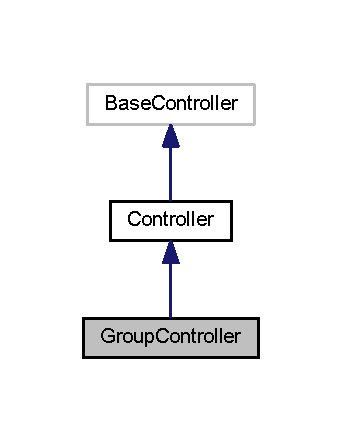
\includegraphics[width=164pt]{class_app_1_1_http_1_1_controllers_1_1_product_1_1_group_controller__inherit__graph}
\end{center}
\end{figure}


Collaboration diagram for Group\+Controller\+:
\nopagebreak
\begin{figure}[H]
\begin{center}
\leavevmode
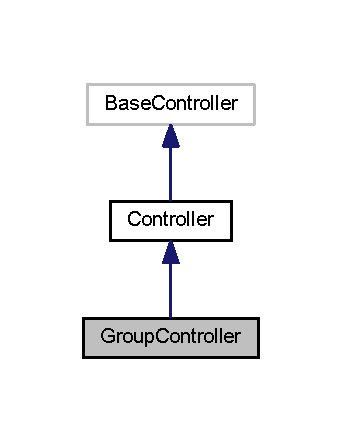
\includegraphics[width=164pt]{class_app_1_1_http_1_1_controllers_1_1_product_1_1_group_controller__coll__graph}
\end{center}
\end{figure}
\subsection*{Public Member Functions}
\begin{DoxyCompactItemize}
\item 
\mbox{\hyperlink{class_app_1_1_http_1_1_controllers_1_1_product_1_1_group_controller_a5b75ba6bc9debb999c0186a31978ec03}{\+\_\+\+\_\+construct}} (\$repository)
\item 
\mbox{\hyperlink{class_app_1_1_http_1_1_controllers_1_1_product_1_1_group_controller_af9d14e4ae6227970ad603987781573ca}{all}} ()
\item 
\mbox{\hyperlink{class_app_1_1_http_1_1_controllers_1_1_product_1_1_group_controller_a50e3bfb586b2f42932a6a93f3fbb0828}{get}} (\$id)
\item 
\mbox{\hyperlink{class_app_1_1_http_1_1_controllers_1_1_product_1_1_group_controller_a4fa811c83f27da01b0d92bdb2a711a13}{create}} (\$request)
\item 
\mbox{\hyperlink{class_app_1_1_http_1_1_controllers_1_1_product_1_1_group_controller_ab7b27a90191560dcef32126b0945db0d}{update}} (\$request)
\item 
\mbox{\hyperlink{class_app_1_1_http_1_1_controllers_1_1_product_1_1_group_controller_a126a3799c44d72393ca4732081306dfd}{delete}} (\$request)
\end{DoxyCompactItemize}


\subsection{Detailed Description}
\mbox{\hyperlink{class_app_1_1_http_1_1_controllers_1_1_controller}{Controller}} for the product groups. 

\subsection{Constructor \& Destructor Documentation}
\mbox{\Hypertarget{class_app_1_1_http_1_1_controllers_1_1_product_1_1_group_controller_a5b75ba6bc9debb999c0186a31978ec03}\label{class_app_1_1_http_1_1_controllers_1_1_product_1_1_group_controller_a5b75ba6bc9debb999c0186a31978ec03}} 
\index{App\+::\+Http\+::\+Controllers\+::\+Product\+::\+Group\+Controller@{App\+::\+Http\+::\+Controllers\+::\+Product\+::\+Group\+Controller}!\+\_\+\+\_\+construct@{\+\_\+\+\_\+construct}}
\index{\+\_\+\+\_\+construct@{\+\_\+\+\_\+construct}!App\+::\+Http\+::\+Controllers\+::\+Product\+::\+Group\+Controller@{App\+::\+Http\+::\+Controllers\+::\+Product\+::\+Group\+Controller}}
\subsubsection{\texorpdfstring{\+\_\+\+\_\+construct()}{\_\_construct()}}
{\footnotesize\ttfamily \+\_\+\+\_\+construct (\begin{DoxyParamCaption}\item[{}]{\$repository }\end{DoxyParamCaption})}

Using dependency injection to get the repository connected to the A\+PI in the app\+\_\+providers.


\begin{DoxyParams}[1]{Parameters}
interface & {\em \$repository} & \\
\hline
\end{DoxyParams}


\subsection{Member Function Documentation}
\mbox{\Hypertarget{class_app_1_1_http_1_1_controllers_1_1_product_1_1_group_controller_af9d14e4ae6227970ad603987781573ca}\label{class_app_1_1_http_1_1_controllers_1_1_product_1_1_group_controller_af9d14e4ae6227970ad603987781573ca}} 
\index{App\+::\+Http\+::\+Controllers\+::\+Product\+::\+Group\+Controller@{App\+::\+Http\+::\+Controllers\+::\+Product\+::\+Group\+Controller}!all@{all}}
\index{all@{all}!App\+::\+Http\+::\+Controllers\+::\+Product\+::\+Group\+Controller@{App\+::\+Http\+::\+Controllers\+::\+Product\+::\+Group\+Controller}}
\subsubsection{\texorpdfstring{all()}{all()}}
{\footnotesize\ttfamily all (\begin{DoxyParamCaption}{ }\end{DoxyParamCaption})}

Returns an array of Group objects.

\begin{DoxyReturn}{Returns}
array 
\end{DoxyReturn}
\mbox{\Hypertarget{class_app_1_1_http_1_1_controllers_1_1_product_1_1_group_controller_a4fa811c83f27da01b0d92bdb2a711a13}\label{class_app_1_1_http_1_1_controllers_1_1_product_1_1_group_controller_a4fa811c83f27da01b0d92bdb2a711a13}} 
\index{App\+::\+Http\+::\+Controllers\+::\+Product\+::\+Group\+Controller@{App\+::\+Http\+::\+Controllers\+::\+Product\+::\+Group\+Controller}!create@{create}}
\index{create@{create}!App\+::\+Http\+::\+Controllers\+::\+Product\+::\+Group\+Controller@{App\+::\+Http\+::\+Controllers\+::\+Product\+::\+Group\+Controller}}
\subsubsection{\texorpdfstring{create()}{create()}}
{\footnotesize\ttfamily create (\begin{DoxyParamCaption}\item[{}]{\$request }\end{DoxyParamCaption})}

Store a new group.

\begin{DoxyReturn}{Returns}
boolean 
\end{DoxyReturn}
\mbox{\Hypertarget{class_app_1_1_http_1_1_controllers_1_1_product_1_1_group_controller_a126a3799c44d72393ca4732081306dfd}\label{class_app_1_1_http_1_1_controllers_1_1_product_1_1_group_controller_a126a3799c44d72393ca4732081306dfd}} 
\index{App\+::\+Http\+::\+Controllers\+::\+Product\+::\+Group\+Controller@{App\+::\+Http\+::\+Controllers\+::\+Product\+::\+Group\+Controller}!delete@{delete}}
\index{delete@{delete}!App\+::\+Http\+::\+Controllers\+::\+Product\+::\+Group\+Controller@{App\+::\+Http\+::\+Controllers\+::\+Product\+::\+Group\+Controller}}
\subsubsection{\texorpdfstring{delete()}{delete()}}
{\footnotesize\ttfamily delete (\begin{DoxyParamCaption}\item[{}]{\$request }\end{DoxyParamCaption})}

Delete a group.

\begin{DoxyReturn}{Returns}
boolean 
\end{DoxyReturn}
\mbox{\Hypertarget{class_app_1_1_http_1_1_controllers_1_1_product_1_1_group_controller_a50e3bfb586b2f42932a6a93f3fbb0828}\label{class_app_1_1_http_1_1_controllers_1_1_product_1_1_group_controller_a50e3bfb586b2f42932a6a93f3fbb0828}} 
\index{App\+::\+Http\+::\+Controllers\+::\+Product\+::\+Group\+Controller@{App\+::\+Http\+::\+Controllers\+::\+Product\+::\+Group\+Controller}!get@{get}}
\index{get@{get}!App\+::\+Http\+::\+Controllers\+::\+Product\+::\+Group\+Controller@{App\+::\+Http\+::\+Controllers\+::\+Product\+::\+Group\+Controller}}
\subsubsection{\texorpdfstring{get()}{get()}}
{\footnotesize\ttfamily get (\begin{DoxyParamCaption}\item[{}]{\$id }\end{DoxyParamCaption})}

Returns an Group Object with the provided id.

\begin{DoxyReturn}{Returns}
object 
\end{DoxyReturn}
\mbox{\Hypertarget{class_app_1_1_http_1_1_controllers_1_1_product_1_1_group_controller_ab7b27a90191560dcef32126b0945db0d}\label{class_app_1_1_http_1_1_controllers_1_1_product_1_1_group_controller_ab7b27a90191560dcef32126b0945db0d}} 
\index{App\+::\+Http\+::\+Controllers\+::\+Product\+::\+Group\+Controller@{App\+::\+Http\+::\+Controllers\+::\+Product\+::\+Group\+Controller}!update@{update}}
\index{update@{update}!App\+::\+Http\+::\+Controllers\+::\+Product\+::\+Group\+Controller@{App\+::\+Http\+::\+Controllers\+::\+Product\+::\+Group\+Controller}}
\subsubsection{\texorpdfstring{update()}{update()}}
{\footnotesize\ttfamily update (\begin{DoxyParamCaption}\item[{}]{\$request }\end{DoxyParamCaption})}

Update a group.

\begin{DoxyReturn}{Returns}
boolean 
\end{DoxyReturn}


The documentation for this class was generated from the following file\+:\begin{DoxyCompactItemize}
\item 
app/\+Http/\+Controllers/\+Product/Group\+Controller.\+php\end{DoxyCompactItemize}

\hypertarget{interface_app_1_1_repositories_1_1_product_1_1_group_repository_interface}{}\section{Group\+Repository\+Interface Interface Reference}
\label{interface_app_1_1_repositories_1_1_product_1_1_group_repository_interface}\index{Group\+Repository\+Interface@{Group\+Repository\+Interface}}
\subsection*{Public Member Functions}
\begin{DoxyCompactItemize}
\item 
\mbox{\hyperlink{interface_app_1_1_repositories_1_1_product_1_1_group_repository_interface_af9d14e4ae6227970ad603987781573ca}{all}} ()
\item 
\mbox{\hyperlink{interface_app_1_1_repositories_1_1_product_1_1_group_repository_interface_a50e3bfb586b2f42932a6a93f3fbb0828}{get}} (\$id)
\item 
\mbox{\hyperlink{interface_app_1_1_repositories_1_1_product_1_1_group_repository_interface_a4fa811c83f27da01b0d92bdb2a711a13}{create}} (\$request)
\item 
\mbox{\hyperlink{interface_app_1_1_repositories_1_1_product_1_1_group_repository_interface_a2aedea52c52e54ba3c4c9f60423e7ef1}{udpate}} (\$request)
\item 
\mbox{\hyperlink{interface_app_1_1_repositories_1_1_product_1_1_group_repository_interface_a126a3799c44d72393ca4732081306dfd}{delete}} (\$request)
\end{DoxyCompactItemize}


\subsection{Detailed Description}
Interface for the Group\+Repository 

\subsection{Member Function Documentation}
\mbox{\Hypertarget{interface_app_1_1_repositories_1_1_product_1_1_group_repository_interface_af9d14e4ae6227970ad603987781573ca}\label{interface_app_1_1_repositories_1_1_product_1_1_group_repository_interface_af9d14e4ae6227970ad603987781573ca}} 
\index{App\+::\+Repositories\+::\+Product\+::\+Group\+Repository\+Interface@{App\+::\+Repositories\+::\+Product\+::\+Group\+Repository\+Interface}!all@{all}}
\index{all@{all}!App\+::\+Repositories\+::\+Product\+::\+Group\+Repository\+Interface@{App\+::\+Repositories\+::\+Product\+::\+Group\+Repository\+Interface}}
\subsubsection{\texorpdfstring{all()}{all()}}
{\footnotesize\ttfamily all (\begin{DoxyParamCaption}{ }\end{DoxyParamCaption})}

Returns an array of Group objects.

\begin{DoxyReturn}{Returns}
array 
\end{DoxyReturn}
\mbox{\Hypertarget{interface_app_1_1_repositories_1_1_product_1_1_group_repository_interface_a4fa811c83f27da01b0d92bdb2a711a13}\label{interface_app_1_1_repositories_1_1_product_1_1_group_repository_interface_a4fa811c83f27da01b0d92bdb2a711a13}} 
\index{App\+::\+Repositories\+::\+Product\+::\+Group\+Repository\+Interface@{App\+::\+Repositories\+::\+Product\+::\+Group\+Repository\+Interface}!create@{create}}
\index{create@{create}!App\+::\+Repositories\+::\+Product\+::\+Group\+Repository\+Interface@{App\+::\+Repositories\+::\+Product\+::\+Group\+Repository\+Interface}}
\subsubsection{\texorpdfstring{create()}{create()}}
{\footnotesize\ttfamily create (\begin{DoxyParamCaption}\item[{}]{\$request }\end{DoxyParamCaption})}

Returns a boolean reflecting the creation status.

\begin{DoxyReturn}{Returns}
boolean 
\end{DoxyReturn}
\mbox{\Hypertarget{interface_app_1_1_repositories_1_1_product_1_1_group_repository_interface_a126a3799c44d72393ca4732081306dfd}\label{interface_app_1_1_repositories_1_1_product_1_1_group_repository_interface_a126a3799c44d72393ca4732081306dfd}} 
\index{App\+::\+Repositories\+::\+Product\+::\+Group\+Repository\+Interface@{App\+::\+Repositories\+::\+Product\+::\+Group\+Repository\+Interface}!delete@{delete}}
\index{delete@{delete}!App\+::\+Repositories\+::\+Product\+::\+Group\+Repository\+Interface@{App\+::\+Repositories\+::\+Product\+::\+Group\+Repository\+Interface}}
\subsubsection{\texorpdfstring{delete()}{delete()}}
{\footnotesize\ttfamily delete (\begin{DoxyParamCaption}\item[{}]{\$request }\end{DoxyParamCaption})}

Returns a boolean reflecting the deletion status.

\begin{DoxyReturn}{Returns}
boolean 
\end{DoxyReturn}
\mbox{\Hypertarget{interface_app_1_1_repositories_1_1_product_1_1_group_repository_interface_a50e3bfb586b2f42932a6a93f3fbb0828}\label{interface_app_1_1_repositories_1_1_product_1_1_group_repository_interface_a50e3bfb586b2f42932a6a93f3fbb0828}} 
\index{App\+::\+Repositories\+::\+Product\+::\+Group\+Repository\+Interface@{App\+::\+Repositories\+::\+Product\+::\+Group\+Repository\+Interface}!get@{get}}
\index{get@{get}!App\+::\+Repositories\+::\+Product\+::\+Group\+Repository\+Interface@{App\+::\+Repositories\+::\+Product\+::\+Group\+Repository\+Interface}}
\subsubsection{\texorpdfstring{get()}{get()}}
{\footnotesize\ttfamily get (\begin{DoxyParamCaption}\item[{}]{\$id }\end{DoxyParamCaption})}

Returns an Group Object with the provided id.

\begin{DoxyReturn}{Returns}
object 
\end{DoxyReturn}
\mbox{\Hypertarget{interface_app_1_1_repositories_1_1_product_1_1_group_repository_interface_a2aedea52c52e54ba3c4c9f60423e7ef1}\label{interface_app_1_1_repositories_1_1_product_1_1_group_repository_interface_a2aedea52c52e54ba3c4c9f60423e7ef1}} 
\index{App\+::\+Repositories\+::\+Product\+::\+Group\+Repository\+Interface@{App\+::\+Repositories\+::\+Product\+::\+Group\+Repository\+Interface}!udpate@{udpate}}
\index{udpate@{udpate}!App\+::\+Repositories\+::\+Product\+::\+Group\+Repository\+Interface@{App\+::\+Repositories\+::\+Product\+::\+Group\+Repository\+Interface}}
\subsubsection{\texorpdfstring{udpate()}{udpate()}}
{\footnotesize\ttfamily udpate (\begin{DoxyParamCaption}\item[{}]{\$request }\end{DoxyParamCaption})}

Returns a boolean reflecting the update status.

\begin{DoxyReturn}{Returns}
boolean 
\end{DoxyReturn}


The documentation for this interface was generated from the following file\+:\begin{DoxyCompactItemize}
\item 
app/\+Repositories/\+Product/Group\+Repository\+Interface.\+php\end{DoxyCompactItemize}

\hypertarget{class_app_1_1_exceptions_1_1_handler}{}\section{Handler Class Reference}
\label{class_app_1_1_exceptions_1_1_handler}\index{Handler@{Handler}}


Inheritance diagram for Handler\+:
\nopagebreak
\begin{figure}[H]
\begin{center}
\leavevmode
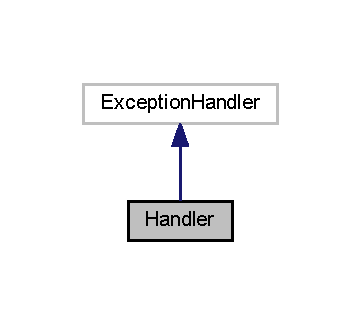
\includegraphics[width=173pt]{class_app_1_1_exceptions_1_1_handler__inherit__graph}
\end{center}
\end{figure}


Collaboration diagram for Handler\+:
\nopagebreak
\begin{figure}[H]
\begin{center}
\leavevmode
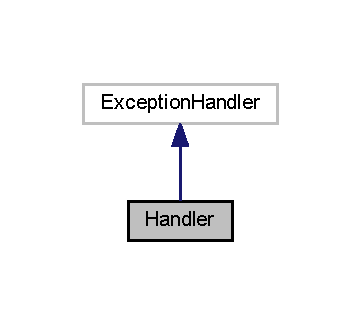
\includegraphics[width=173pt]{class_app_1_1_exceptions_1_1_handler__coll__graph}
\end{center}
\end{figure}
\subsection*{Public Member Functions}
\begin{DoxyCompactItemize}
\item 
\mbox{\hyperlink{class_app_1_1_exceptions_1_1_handler_ac0ed66852194d5c444146cec8eec8ca4}{report}} (Exception \$e)
\item 
\mbox{\hyperlink{class_app_1_1_exceptions_1_1_handler_a7f412df510b6ecdb4aac9455d71af13a}{render}} (\$request, Exception \$e)
\end{DoxyCompactItemize}
\subsection*{Protected Attributes}
\begin{DoxyCompactItemize}
\item 
{\bfseries \$dont\+Report}
\end{DoxyCompactItemize}


\subsection{Member Function Documentation}
\mbox{\Hypertarget{class_app_1_1_exceptions_1_1_handler_a7f412df510b6ecdb4aac9455d71af13a}\label{class_app_1_1_exceptions_1_1_handler_a7f412df510b6ecdb4aac9455d71af13a}} 
\index{App\+::\+Exceptions\+::\+Handler@{App\+::\+Exceptions\+::\+Handler}!render@{render}}
\index{render@{render}!App\+::\+Exceptions\+::\+Handler@{App\+::\+Exceptions\+::\+Handler}}
\subsubsection{\texorpdfstring{render()}{render()}}
{\footnotesize\ttfamily render (\begin{DoxyParamCaption}\item[{}]{\$request,  }\item[{Exception}]{\$e }\end{DoxyParamCaption})}

Render an exception into an H\+T\+TP response.


\begin{DoxyParams}[1]{Parameters}
\textbackslash{}\+Illuminate\textbackslash{}\+Http\textbackslash{}\+Request & {\em \$request} & \\
\hline
\textbackslash{}\+Exception & {\em \$e} & \\
\hline
\end{DoxyParams}
\begin{DoxyReturn}{Returns}

\end{DoxyReturn}
\mbox{\Hypertarget{class_app_1_1_exceptions_1_1_handler_ac0ed66852194d5c444146cec8eec8ca4}\label{class_app_1_1_exceptions_1_1_handler_ac0ed66852194d5c444146cec8eec8ca4}} 
\index{App\+::\+Exceptions\+::\+Handler@{App\+::\+Exceptions\+::\+Handler}!report@{report}}
\index{report@{report}!App\+::\+Exceptions\+::\+Handler@{App\+::\+Exceptions\+::\+Handler}}
\subsubsection{\texorpdfstring{report()}{report()}}
{\footnotesize\ttfamily report (\begin{DoxyParamCaption}\item[{Exception}]{\$e }\end{DoxyParamCaption})}

Report or log an exception.

This is a great spot to send exceptions to Sentry, Bugsnag, etc.


\begin{DoxyParams}[1]{Parameters}
\textbackslash{}\+Exception & {\em \$e} & \\
\hline
\end{DoxyParams}
\begin{DoxyReturn}{Returns}
void 
\end{DoxyReturn}


\subsection{Field Documentation}
\mbox{\Hypertarget{class_app_1_1_exceptions_1_1_handler_ae8da729578a9bcab20236efc2404d62e}\label{class_app_1_1_exceptions_1_1_handler_ae8da729578a9bcab20236efc2404d62e}} 
\index{App\+::\+Exceptions\+::\+Handler@{App\+::\+Exceptions\+::\+Handler}!\$dont\+Report@{\$dont\+Report}}
\index{\$dont\+Report@{\$dont\+Report}!App\+::\+Exceptions\+::\+Handler@{App\+::\+Exceptions\+::\+Handler}}
\subsubsection{\texorpdfstring{\$dont\+Report}{$dontReport}}
{\footnotesize\ttfamily \$dont\+Report\hspace{0.3cm}{\ttfamily [protected]}}

{\bfseries Initial value\+:}
\begin{DoxyCode}
= [
        AuthorizationException::class,
        HttpException::class,
        ModelNotFoundException::class,
        ValidationException::class,
    ]
\end{DoxyCode}


The documentation for this class was generated from the following file\+:\begin{DoxyCompactItemize}
\item 
app/\+Exceptions/Handler.\+php\end{DoxyCompactItemize}

\hypertarget{class_app_1_1_models_1_1_product_1_1_ingredient}{}\section{Ingredient Class Reference}
\label{class_app_1_1_models_1_1_product_1_1_ingredient}\index{Ingredient@{Ingredient}}


Inheritance diagram for Ingredient\+:
\nopagebreak
\begin{figure}[H]
\begin{center}
\leavevmode
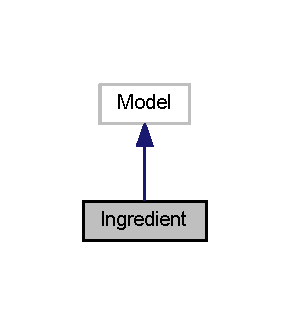
\includegraphics[width=139pt]{class_app_1_1_models_1_1_product_1_1_ingredient__inherit__graph}
\end{center}
\end{figure}


Collaboration diagram for Ingredient\+:
\nopagebreak
\begin{figure}[H]
\begin{center}
\leavevmode
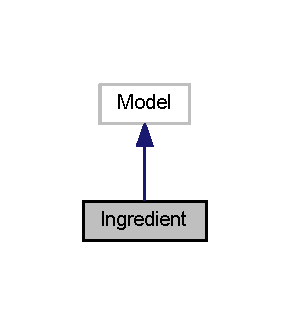
\includegraphics[width=139pt]{class_app_1_1_models_1_1_product_1_1_ingredient__coll__graph}
\end{center}
\end{figure}
\subsection*{Protected Attributes}
\begin{DoxyCompactItemize}
\item 
\mbox{\Hypertarget{class_app_1_1_models_1_1_product_1_1_ingredient_ae8876a14058f368335baccf35af4a22b}\label{class_app_1_1_models_1_1_product_1_1_ingredient_ae8876a14058f368335baccf35af4a22b}} 
{\bfseries \$table} = \textquotesingle{}product\+\_\+ingredients\textquotesingle{}
\item 
{\bfseries \$fillabe}
\end{DoxyCompactItemize}


\subsection{Detailed Description}
Represents the ingredients a product may have. Will be useful for selecting just a few ingredients in the order instead of all. Could be meat, chicken, cheese, salad.

Accepts name\+: string, status\+: tiny\+Integer. Status will be indicate if the ingredient is available in stock. 

\subsection{Field Documentation}
\mbox{\Hypertarget{class_app_1_1_models_1_1_product_1_1_ingredient_ac5c29ce22e45a54200f88204e498d290}\label{class_app_1_1_models_1_1_product_1_1_ingredient_ac5c29ce22e45a54200f88204e498d290}} 
\index{App\+::\+Models\+::\+Product\+::\+Ingredient@{App\+::\+Models\+::\+Product\+::\+Ingredient}!\$fillabe@{\$fillabe}}
\index{\$fillabe@{\$fillabe}!App\+::\+Models\+::\+Product\+::\+Ingredient@{App\+::\+Models\+::\+Product\+::\+Ingredient}}
\subsubsection{\texorpdfstring{\$fillabe}{$fillabe}}
{\footnotesize\ttfamily \$fillabe\hspace{0.3cm}{\ttfamily [protected]}}

{\bfseries Initial value\+:}
\begin{DoxyCode}
= [
        \textcolor{stringliteral}{'name'},
        \textcolor{stringliteral}{'status'}
    ]
\end{DoxyCode}


The documentation for this class was generated from the following file\+:\begin{DoxyCompactItemize}
\item 
app/\+Models/\+Product/Ingredient.\+php\end{DoxyCompactItemize}

\hypertarget{class_app_1_1_http_1_1_controllers_1_1_product_1_1_ingredient_controller}{}\section{Ingredient\+Controller Class Reference}
\label{class_app_1_1_http_1_1_controllers_1_1_product_1_1_ingredient_controller}\index{Ingredient\+Controller@{Ingredient\+Controller}}


Inheritance diagram for Ingredient\+Controller\+:
\nopagebreak
\begin{figure}[H]
\begin{center}
\leavevmode
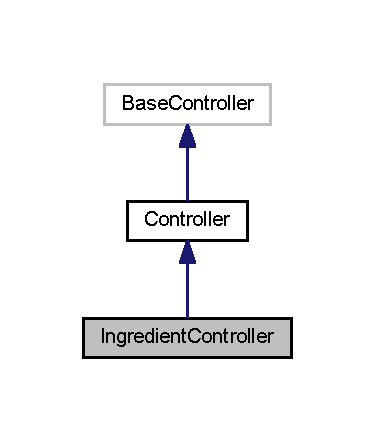
\includegraphics[width=180pt]{class_app_1_1_http_1_1_controllers_1_1_product_1_1_ingredient_controller__inherit__graph}
\end{center}
\end{figure}


Collaboration diagram for Ingredient\+Controller\+:
\nopagebreak
\begin{figure}[H]
\begin{center}
\leavevmode
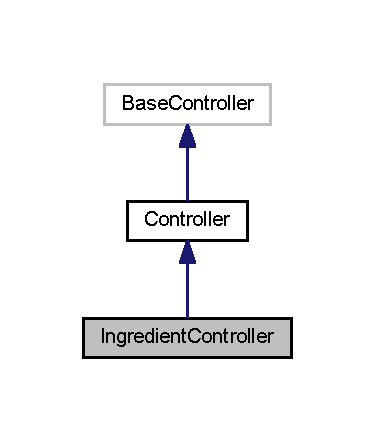
\includegraphics[width=180pt]{class_app_1_1_http_1_1_controllers_1_1_product_1_1_ingredient_controller__coll__graph}
\end{center}
\end{figure}
\subsection*{Public Member Functions}
\begin{DoxyCompactItemize}
\item 
\mbox{\hyperlink{class_app_1_1_http_1_1_controllers_1_1_product_1_1_ingredient_controller_a5b75ba6bc9debb999c0186a31978ec03}{\+\_\+\+\_\+construct}} (\$repository)
\item 
\mbox{\hyperlink{class_app_1_1_http_1_1_controllers_1_1_product_1_1_ingredient_controller_af9d14e4ae6227970ad603987781573ca}{all}} ()
\item 
\mbox{\hyperlink{class_app_1_1_http_1_1_controllers_1_1_product_1_1_ingredient_controller_a50e3bfb586b2f42932a6a93f3fbb0828}{get}} (\$id)
\item 
\mbox{\hyperlink{class_app_1_1_http_1_1_controllers_1_1_product_1_1_ingredient_controller_a4fa811c83f27da01b0d92bdb2a711a13}{create}} (\$request)
\item 
\mbox{\hyperlink{class_app_1_1_http_1_1_controllers_1_1_product_1_1_ingredient_controller_ab7b27a90191560dcef32126b0945db0d}{update}} (\$request)
\item 
\mbox{\hyperlink{class_app_1_1_http_1_1_controllers_1_1_product_1_1_ingredient_controller_a126a3799c44d72393ca4732081306dfd}{delete}} (\$request)
\end{DoxyCompactItemize}


\subsection{Detailed Description}
\mbox{\hyperlink{class_app_1_1_http_1_1_controllers_1_1_controller}{Controller}} for the product ingredients. 

\subsection{Constructor \& Destructor Documentation}
\mbox{\Hypertarget{class_app_1_1_http_1_1_controllers_1_1_product_1_1_ingredient_controller_a5b75ba6bc9debb999c0186a31978ec03}\label{class_app_1_1_http_1_1_controllers_1_1_product_1_1_ingredient_controller_a5b75ba6bc9debb999c0186a31978ec03}} 
\index{App\+::\+Http\+::\+Controllers\+::\+Product\+::\+Ingredient\+Controller@{App\+::\+Http\+::\+Controllers\+::\+Product\+::\+Ingredient\+Controller}!\+\_\+\+\_\+construct@{\+\_\+\+\_\+construct}}
\index{\+\_\+\+\_\+construct@{\+\_\+\+\_\+construct}!App\+::\+Http\+::\+Controllers\+::\+Product\+::\+Ingredient\+Controller@{App\+::\+Http\+::\+Controllers\+::\+Product\+::\+Ingredient\+Controller}}
\subsubsection{\texorpdfstring{\+\_\+\+\_\+construct()}{\_\_construct()}}
{\footnotesize\ttfamily \+\_\+\+\_\+construct (\begin{DoxyParamCaption}\item[{}]{\$repository }\end{DoxyParamCaption})}

Using dependency injection to get the repository connected to the A\+PI in the app\+\_\+providers.


\begin{DoxyParams}[1]{Parameters}
interface & {\em \$repository} & \\
\hline
\end{DoxyParams}


\subsection{Member Function Documentation}
\mbox{\Hypertarget{class_app_1_1_http_1_1_controllers_1_1_product_1_1_ingredient_controller_af9d14e4ae6227970ad603987781573ca}\label{class_app_1_1_http_1_1_controllers_1_1_product_1_1_ingredient_controller_af9d14e4ae6227970ad603987781573ca}} 
\index{App\+::\+Http\+::\+Controllers\+::\+Product\+::\+Ingredient\+Controller@{App\+::\+Http\+::\+Controllers\+::\+Product\+::\+Ingredient\+Controller}!all@{all}}
\index{all@{all}!App\+::\+Http\+::\+Controllers\+::\+Product\+::\+Ingredient\+Controller@{App\+::\+Http\+::\+Controllers\+::\+Product\+::\+Ingredient\+Controller}}
\subsubsection{\texorpdfstring{all()}{all()}}
{\footnotesize\ttfamily all (\begin{DoxyParamCaption}{ }\end{DoxyParamCaption})}

Returns an array of Ingredient objects.

\begin{DoxyReturn}{Returns}
array 
\end{DoxyReturn}
\mbox{\Hypertarget{class_app_1_1_http_1_1_controllers_1_1_product_1_1_ingredient_controller_a4fa811c83f27da01b0d92bdb2a711a13}\label{class_app_1_1_http_1_1_controllers_1_1_product_1_1_ingredient_controller_a4fa811c83f27da01b0d92bdb2a711a13}} 
\index{App\+::\+Http\+::\+Controllers\+::\+Product\+::\+Ingredient\+Controller@{App\+::\+Http\+::\+Controllers\+::\+Product\+::\+Ingredient\+Controller}!create@{create}}
\index{create@{create}!App\+::\+Http\+::\+Controllers\+::\+Product\+::\+Ingredient\+Controller@{App\+::\+Http\+::\+Controllers\+::\+Product\+::\+Ingredient\+Controller}}
\subsubsection{\texorpdfstring{create()}{create()}}
{\footnotesize\ttfamily create (\begin{DoxyParamCaption}\item[{}]{\$request }\end{DoxyParamCaption})}

Store a new ingredient.

\begin{DoxyReturn}{Returns}
boolean 
\end{DoxyReturn}
\mbox{\Hypertarget{class_app_1_1_http_1_1_controllers_1_1_product_1_1_ingredient_controller_a126a3799c44d72393ca4732081306dfd}\label{class_app_1_1_http_1_1_controllers_1_1_product_1_1_ingredient_controller_a126a3799c44d72393ca4732081306dfd}} 
\index{App\+::\+Http\+::\+Controllers\+::\+Product\+::\+Ingredient\+Controller@{App\+::\+Http\+::\+Controllers\+::\+Product\+::\+Ingredient\+Controller}!delete@{delete}}
\index{delete@{delete}!App\+::\+Http\+::\+Controllers\+::\+Product\+::\+Ingredient\+Controller@{App\+::\+Http\+::\+Controllers\+::\+Product\+::\+Ingredient\+Controller}}
\subsubsection{\texorpdfstring{delete()}{delete()}}
{\footnotesize\ttfamily delete (\begin{DoxyParamCaption}\item[{}]{\$request }\end{DoxyParamCaption})}

Delete an ingredient.

\begin{DoxyReturn}{Returns}
boolean 
\end{DoxyReturn}
\mbox{\Hypertarget{class_app_1_1_http_1_1_controllers_1_1_product_1_1_ingredient_controller_a50e3bfb586b2f42932a6a93f3fbb0828}\label{class_app_1_1_http_1_1_controllers_1_1_product_1_1_ingredient_controller_a50e3bfb586b2f42932a6a93f3fbb0828}} 
\index{App\+::\+Http\+::\+Controllers\+::\+Product\+::\+Ingredient\+Controller@{App\+::\+Http\+::\+Controllers\+::\+Product\+::\+Ingredient\+Controller}!get@{get}}
\index{get@{get}!App\+::\+Http\+::\+Controllers\+::\+Product\+::\+Ingredient\+Controller@{App\+::\+Http\+::\+Controllers\+::\+Product\+::\+Ingredient\+Controller}}
\subsubsection{\texorpdfstring{get()}{get()}}
{\footnotesize\ttfamily get (\begin{DoxyParamCaption}\item[{}]{\$id }\end{DoxyParamCaption})}

Returns an Ingredient Object with the provided id.

\begin{DoxyReturn}{Returns}
object 
\end{DoxyReturn}
\mbox{\Hypertarget{class_app_1_1_http_1_1_controllers_1_1_product_1_1_ingredient_controller_ab7b27a90191560dcef32126b0945db0d}\label{class_app_1_1_http_1_1_controllers_1_1_product_1_1_ingredient_controller_ab7b27a90191560dcef32126b0945db0d}} 
\index{App\+::\+Http\+::\+Controllers\+::\+Product\+::\+Ingredient\+Controller@{App\+::\+Http\+::\+Controllers\+::\+Product\+::\+Ingredient\+Controller}!update@{update}}
\index{update@{update}!App\+::\+Http\+::\+Controllers\+::\+Product\+::\+Ingredient\+Controller@{App\+::\+Http\+::\+Controllers\+::\+Product\+::\+Ingredient\+Controller}}
\subsubsection{\texorpdfstring{update()}{update()}}
{\footnotesize\ttfamily update (\begin{DoxyParamCaption}\item[{}]{\$request }\end{DoxyParamCaption})}

Update an ingredient.

\begin{DoxyReturn}{Returns}
boolean 
\end{DoxyReturn}


The documentation for this class was generated from the following file\+:\begin{DoxyCompactItemize}
\item 
app/\+Http/\+Controllers/\+Product/Ingredient\+Controller.\+php\end{DoxyCompactItemize}

\hypertarget{interface_app_1_1_repositories_1_1_product_1_1_ingredient_repository_interface}{}\section{Ingredient\+Repository\+Interface Interface Reference}
\label{interface_app_1_1_repositories_1_1_product_1_1_ingredient_repository_interface}\index{Ingredient\+Repository\+Interface@{Ingredient\+Repository\+Interface}}
\subsection*{Public Member Functions}
\begin{DoxyCompactItemize}
\item 
\mbox{\hyperlink{interface_app_1_1_repositories_1_1_product_1_1_ingredient_repository_interface_af9d14e4ae6227970ad603987781573ca}{all}} ()
\item 
\mbox{\hyperlink{interface_app_1_1_repositories_1_1_product_1_1_ingredient_repository_interface_a50e3bfb586b2f42932a6a93f3fbb0828}{get}} (\$id)
\item 
\mbox{\hyperlink{interface_app_1_1_repositories_1_1_product_1_1_ingredient_repository_interface_a4fa811c83f27da01b0d92bdb2a711a13}{create}} (\$request)
\item 
\mbox{\hyperlink{interface_app_1_1_repositories_1_1_product_1_1_ingredient_repository_interface_a2aedea52c52e54ba3c4c9f60423e7ef1}{udpate}} (\$request)
\item 
\mbox{\hyperlink{interface_app_1_1_repositories_1_1_product_1_1_ingredient_repository_interface_a126a3799c44d72393ca4732081306dfd}{delete}} (\$request)
\end{DoxyCompactItemize}


\subsection{Detailed Description}
Interface for the Ingredient\+Repository 

\subsection{Member Function Documentation}
\mbox{\Hypertarget{interface_app_1_1_repositories_1_1_product_1_1_ingredient_repository_interface_af9d14e4ae6227970ad603987781573ca}\label{interface_app_1_1_repositories_1_1_product_1_1_ingredient_repository_interface_af9d14e4ae6227970ad603987781573ca}} 
\index{App\+::\+Repositories\+::\+Product\+::\+Ingredient\+Repository\+Interface@{App\+::\+Repositories\+::\+Product\+::\+Ingredient\+Repository\+Interface}!all@{all}}
\index{all@{all}!App\+::\+Repositories\+::\+Product\+::\+Ingredient\+Repository\+Interface@{App\+::\+Repositories\+::\+Product\+::\+Ingredient\+Repository\+Interface}}
\subsubsection{\texorpdfstring{all()}{all()}}
{\footnotesize\ttfamily all (\begin{DoxyParamCaption}{ }\end{DoxyParamCaption})}

Returns an array of Ingredient objects.

\begin{DoxyReturn}{Returns}
array 
\end{DoxyReturn}
\mbox{\Hypertarget{interface_app_1_1_repositories_1_1_product_1_1_ingredient_repository_interface_a4fa811c83f27da01b0d92bdb2a711a13}\label{interface_app_1_1_repositories_1_1_product_1_1_ingredient_repository_interface_a4fa811c83f27da01b0d92bdb2a711a13}} 
\index{App\+::\+Repositories\+::\+Product\+::\+Ingredient\+Repository\+Interface@{App\+::\+Repositories\+::\+Product\+::\+Ingredient\+Repository\+Interface}!create@{create}}
\index{create@{create}!App\+::\+Repositories\+::\+Product\+::\+Ingredient\+Repository\+Interface@{App\+::\+Repositories\+::\+Product\+::\+Ingredient\+Repository\+Interface}}
\subsubsection{\texorpdfstring{create()}{create()}}
{\footnotesize\ttfamily create (\begin{DoxyParamCaption}\item[{}]{\$request }\end{DoxyParamCaption})}

Returns a boolean reflecting the creation status.

\begin{DoxyReturn}{Returns}
boolean 
\end{DoxyReturn}
\mbox{\Hypertarget{interface_app_1_1_repositories_1_1_product_1_1_ingredient_repository_interface_a126a3799c44d72393ca4732081306dfd}\label{interface_app_1_1_repositories_1_1_product_1_1_ingredient_repository_interface_a126a3799c44d72393ca4732081306dfd}} 
\index{App\+::\+Repositories\+::\+Product\+::\+Ingredient\+Repository\+Interface@{App\+::\+Repositories\+::\+Product\+::\+Ingredient\+Repository\+Interface}!delete@{delete}}
\index{delete@{delete}!App\+::\+Repositories\+::\+Product\+::\+Ingredient\+Repository\+Interface@{App\+::\+Repositories\+::\+Product\+::\+Ingredient\+Repository\+Interface}}
\subsubsection{\texorpdfstring{delete()}{delete()}}
{\footnotesize\ttfamily delete (\begin{DoxyParamCaption}\item[{}]{\$request }\end{DoxyParamCaption})}

Returns a boolean reflecting the deletion status.

\begin{DoxyReturn}{Returns}
boolean 
\end{DoxyReturn}
\mbox{\Hypertarget{interface_app_1_1_repositories_1_1_product_1_1_ingredient_repository_interface_a50e3bfb586b2f42932a6a93f3fbb0828}\label{interface_app_1_1_repositories_1_1_product_1_1_ingredient_repository_interface_a50e3bfb586b2f42932a6a93f3fbb0828}} 
\index{App\+::\+Repositories\+::\+Product\+::\+Ingredient\+Repository\+Interface@{App\+::\+Repositories\+::\+Product\+::\+Ingredient\+Repository\+Interface}!get@{get}}
\index{get@{get}!App\+::\+Repositories\+::\+Product\+::\+Ingredient\+Repository\+Interface@{App\+::\+Repositories\+::\+Product\+::\+Ingredient\+Repository\+Interface}}
\subsubsection{\texorpdfstring{get()}{get()}}
{\footnotesize\ttfamily get (\begin{DoxyParamCaption}\item[{}]{\$id }\end{DoxyParamCaption})}

Returns an Ingredient Object with the provided id.

\begin{DoxyReturn}{Returns}
object 
\end{DoxyReturn}
\mbox{\Hypertarget{interface_app_1_1_repositories_1_1_product_1_1_ingredient_repository_interface_a2aedea52c52e54ba3c4c9f60423e7ef1}\label{interface_app_1_1_repositories_1_1_product_1_1_ingredient_repository_interface_a2aedea52c52e54ba3c4c9f60423e7ef1}} 
\index{App\+::\+Repositories\+::\+Product\+::\+Ingredient\+Repository\+Interface@{App\+::\+Repositories\+::\+Product\+::\+Ingredient\+Repository\+Interface}!udpate@{udpate}}
\index{udpate@{udpate}!App\+::\+Repositories\+::\+Product\+::\+Ingredient\+Repository\+Interface@{App\+::\+Repositories\+::\+Product\+::\+Ingredient\+Repository\+Interface}}
\subsubsection{\texorpdfstring{udpate()}{udpate()}}
{\footnotesize\ttfamily udpate (\begin{DoxyParamCaption}\item[{}]{\$request }\end{DoxyParamCaption})}

Returns a boolean reflecting the update status.

\begin{DoxyReturn}{Returns}
boolean 
\end{DoxyReturn}


The documentation for this interface was generated from the following file\+:\begin{DoxyCompactItemize}
\item 
app/\+Repositories/\+Product/Ingredient\+Repository\+Interface.\+php\end{DoxyCompactItemize}

\hypertarget{class_app_1_1_console_1_1_kernel}{}\section{Kernel Class Reference}
\label{class_app_1_1_console_1_1_kernel}\index{Kernel@{Kernel}}


Inheritance diagram for Kernel\+:
\nopagebreak
\begin{figure}[H]
\begin{center}
\leavevmode
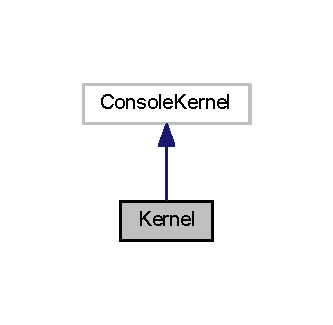
\includegraphics[width=160pt]{class_app_1_1_console_1_1_kernel__inherit__graph}
\end{center}
\end{figure}


Collaboration diagram for Kernel\+:
\nopagebreak
\begin{figure}[H]
\begin{center}
\leavevmode
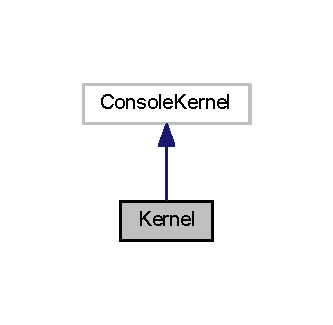
\includegraphics[width=160pt]{class_app_1_1_console_1_1_kernel__coll__graph}
\end{center}
\end{figure}
\subsection*{Protected Member Functions}
\begin{DoxyCompactItemize}
\item 
\mbox{\hyperlink{class_app_1_1_console_1_1_kernel_ac8f0af578c80277b7a25381c6a9e268c}{schedule}} (Schedule \$schedule)
\end{DoxyCompactItemize}
\subsection*{Protected Attributes}
\begin{DoxyCompactItemize}
\item 
{\bfseries \$commands}
\end{DoxyCompactItemize}


\subsection{Member Function Documentation}
\mbox{\Hypertarget{class_app_1_1_console_1_1_kernel_ac8f0af578c80277b7a25381c6a9e268c}\label{class_app_1_1_console_1_1_kernel_ac8f0af578c80277b7a25381c6a9e268c}} 
\index{App\+::\+Console\+::\+Kernel@{App\+::\+Console\+::\+Kernel}!schedule@{schedule}}
\index{schedule@{schedule}!App\+::\+Console\+::\+Kernel@{App\+::\+Console\+::\+Kernel}}
\subsubsection{\texorpdfstring{schedule()}{schedule()}}
{\footnotesize\ttfamily schedule (\begin{DoxyParamCaption}\item[{Schedule}]{\$schedule }\end{DoxyParamCaption})\hspace{0.3cm}{\ttfamily [protected]}}

Define the application\textquotesingle{}s command schedule.


\begin{DoxyParams}[1]{Parameters}
\textbackslash{}\+Illuminate\textbackslash{}\+Console\textbackslash{}\+Scheduling\textbackslash{}\+Schedule & {\em \$schedule} & \\
\hline
\end{DoxyParams}
\begin{DoxyReturn}{Returns}
void 
\end{DoxyReturn}


\subsection{Field Documentation}
\mbox{\Hypertarget{class_app_1_1_console_1_1_kernel_ab63cd62b3b65fd223b6f3d57b6ca754d}\label{class_app_1_1_console_1_1_kernel_ab63cd62b3b65fd223b6f3d57b6ca754d}} 
\index{App\+::\+Console\+::\+Kernel@{App\+::\+Console\+::\+Kernel}!\$commands@{\$commands}}
\index{\$commands@{\$commands}!App\+::\+Console\+::\+Kernel@{App\+::\+Console\+::\+Kernel}}
\subsubsection{\texorpdfstring{\$commands}{$commands}}
{\footnotesize\ttfamily \$commands\hspace{0.3cm}{\ttfamily [protected]}}

{\bfseries Initial value\+:}
\begin{DoxyCode}
= [
        
    ]
\end{DoxyCode}


The documentation for this class was generated from the following file\+:\begin{DoxyCompactItemize}
\item 
app/\+Console/Kernel.\+php\end{DoxyCompactItemize}

\hypertarget{class_app_1_1_models_1_1_order}{}\section{Order Class Reference}
\label{class_app_1_1_models_1_1_order}\index{Order@{Order}}


Inheritance diagram for Order\+:
\nopagebreak
\begin{figure}[H]
\begin{center}
\leavevmode
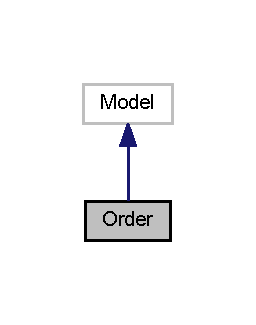
\includegraphics[width=123pt]{class_app_1_1_models_1_1_order__inherit__graph}
\end{center}
\end{figure}


Collaboration diagram for Order\+:
\nopagebreak
\begin{figure}[H]
\begin{center}
\leavevmode
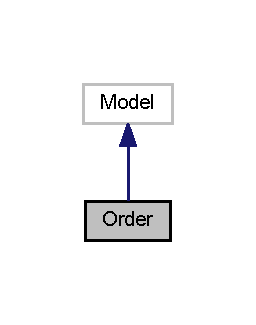
\includegraphics[width=123pt]{class_app_1_1_models_1_1_order__coll__graph}
\end{center}
\end{figure}
\subsection*{Public Member Functions}
\begin{DoxyCompactItemize}
\item 
\mbox{\hyperlink{class_app_1_1_models_1_1_order_af3296e61356149835fcdba50e4075f56}{get\+Card}} ()
\item 
\mbox{\hyperlink{class_app_1_1_models_1_1_order_aa0dd4bf57d57bc2a3697e40c9f6bddce}{get\+Table}} ()
\item 
\mbox{\hyperlink{class_app_1_1_models_1_1_order_aa314a2ddd62ccb42f5a3f80ee8c316e1}{waiters}} ()
\item 
\mbox{\hyperlink{class_app_1_1_models_1_1_order_a9686a480a1adb1923d64e71cf0624275}{get\+Products}} ()
\end{DoxyCompactItemize}
\subsection*{Protected Attributes}
\begin{DoxyCompactItemize}
\item 
\mbox{\Hypertarget{class_app_1_1_models_1_1_order_ae8876a14058f368335baccf35af4a22b}\label{class_app_1_1_models_1_1_order_ae8876a14058f368335baccf35af4a22b}} 
{\bfseries \$table} = \textquotesingle{}orders\textquotesingle{}
\item 
{\bfseries \$fillabe}
\end{DoxyCompactItemize}


\subsection{Detailed Description}
Represents an order. It\textquotesingle{}s connected to several other classes\+: \mbox{\hyperlink{class_app_1_1_models_1_1_card}{Card}}, \mbox{\hyperlink{class_app_1_1_models_1_1_table}{Table}}, \mbox{\hyperlink{class_app_1_1_models_1_1_waiter}{Waiter}}, Product.

Accepts name\+: string, card\+\_\+id\+: integer, table\+\_\+id\+: integer, print\+\_\+status\+: tiny\+Integer, total\+\_\+value\+: double, date\+: Date, status\+: tiny\+Integer. Print Status represents if the order was already printed in a scanner, is being printed or indicates an error. Status represents if the order is still open or was already closed. 

\subsection{Member Function Documentation}
\mbox{\Hypertarget{class_app_1_1_models_1_1_order_af3296e61356149835fcdba50e4075f56}\label{class_app_1_1_models_1_1_order_af3296e61356149835fcdba50e4075f56}} 
\index{App\+::\+Models\+::\+Order@{App\+::\+Models\+::\+Order}!get\+Card@{get\+Card}}
\index{get\+Card@{get\+Card}!App\+::\+Models\+::\+Order@{App\+::\+Models\+::\+Order}}
\subsubsection{\texorpdfstring{get\+Card()}{getCard()}}
{\footnotesize\ttfamily get\+Card (\begin{DoxyParamCaption}{ }\end{DoxyParamCaption})}

Returns the \mbox{\hyperlink{class_app_1_1_models_1_1_card}{Card}} Object used in the order.

\begin{DoxyReturn}{Returns}
object 
\end{DoxyReturn}
\mbox{\Hypertarget{class_app_1_1_models_1_1_order_a9686a480a1adb1923d64e71cf0624275}\label{class_app_1_1_models_1_1_order_a9686a480a1adb1923d64e71cf0624275}} 
\index{App\+::\+Models\+::\+Order@{App\+::\+Models\+::\+Order}!get\+Products@{get\+Products}}
\index{get\+Products@{get\+Products}!App\+::\+Models\+::\+Order@{App\+::\+Models\+::\+Order}}
\subsubsection{\texorpdfstring{get\+Products()}{getProducts()}}
{\footnotesize\ttfamily get\+Products (\begin{DoxyParamCaption}{ }\end{DoxyParamCaption})}

Returns an array of Product of the order.

\begin{DoxyReturn}{Returns}
array 
\end{DoxyReturn}
\mbox{\Hypertarget{class_app_1_1_models_1_1_order_aa0dd4bf57d57bc2a3697e40c9f6bddce}\label{class_app_1_1_models_1_1_order_aa0dd4bf57d57bc2a3697e40c9f6bddce}} 
\index{App\+::\+Models\+::\+Order@{App\+::\+Models\+::\+Order}!get\+Table@{get\+Table}}
\index{get\+Table@{get\+Table}!App\+::\+Models\+::\+Order@{App\+::\+Models\+::\+Order}}
\subsubsection{\texorpdfstring{get\+Table()}{getTable()}}
{\footnotesize\ttfamily get\+Table (\begin{DoxyParamCaption}{ }\end{DoxyParamCaption})}

Returns the \mbox{\hyperlink{class_app_1_1_models_1_1_table}{Table}} Object for the order.

\begin{DoxyReturn}{Returns}
object 
\end{DoxyReturn}
\mbox{\Hypertarget{class_app_1_1_models_1_1_order_aa314a2ddd62ccb42f5a3f80ee8c316e1}\label{class_app_1_1_models_1_1_order_aa314a2ddd62ccb42f5a3f80ee8c316e1}} 
\index{App\+::\+Models\+::\+Order@{App\+::\+Models\+::\+Order}!waiters@{waiters}}
\index{waiters@{waiters}!App\+::\+Models\+::\+Order@{App\+::\+Models\+::\+Order}}
\subsubsection{\texorpdfstring{waiters()}{waiters()}}
{\footnotesize\ttfamily waiters (\begin{DoxyParamCaption}{ }\end{DoxyParamCaption})}

Returns an array of \mbox{\hyperlink{class_app_1_1_models_1_1_waiter}{Waiter}} objects related to this \mbox{\hyperlink{class_app_1_1_models_1_1_order}{Order}}.

\begin{DoxyReturn}{Returns}
array 
\end{DoxyReturn}


\subsection{Field Documentation}
\mbox{\Hypertarget{class_app_1_1_models_1_1_order_ac5c29ce22e45a54200f88204e498d290}\label{class_app_1_1_models_1_1_order_ac5c29ce22e45a54200f88204e498d290}} 
\index{App\+::\+Models\+::\+Order@{App\+::\+Models\+::\+Order}!\$fillabe@{\$fillabe}}
\index{\$fillabe@{\$fillabe}!App\+::\+Models\+::\+Order@{App\+::\+Models\+::\+Order}}
\subsubsection{\texorpdfstring{\$fillabe}{$fillabe}}
{\footnotesize\ttfamily \$fillabe\hspace{0.3cm}{\ttfamily [protected]}}

{\bfseries Initial value\+:}
\begin{DoxyCode}
= [
        \textcolor{stringliteral}{'name'},
        \textcolor{stringliteral}{'card\_id'},
        \textcolor{stringliteral}{'table\_id'},
        \textcolor{stringliteral}{'print\_status'},
        \textcolor{stringliteral}{'total\_value'},
        \textcolor{stringliteral}{'date'},
        \textcolor{stringliteral}{'status'}
    ]
\end{DoxyCode}


The documentation for this class was generated from the following file\+:\begin{DoxyCompactItemize}
\item 
app/\+Models/Order.\+php\end{DoxyCompactItemize}

\hypertarget{class_app_1_1_http_1_1_controllers_1_1_order_controller}{}\section{Order\+Controller Class Reference}
\label{class_app_1_1_http_1_1_controllers_1_1_order_controller}\index{Order\+Controller@{Order\+Controller}}


Inheritance diagram for Order\+Controller\+:
\nopagebreak
\begin{figure}[H]
\begin{center}
\leavevmode
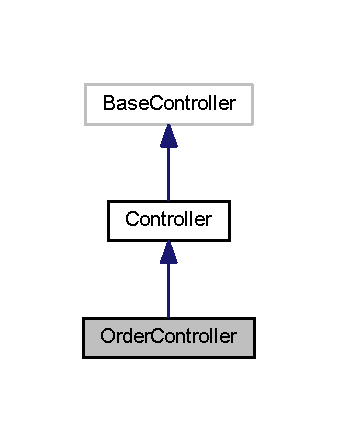
\includegraphics[width=162pt]{class_app_1_1_http_1_1_controllers_1_1_order_controller__inherit__graph}
\end{center}
\end{figure}


Collaboration diagram for Order\+Controller\+:
\nopagebreak
\begin{figure}[H]
\begin{center}
\leavevmode
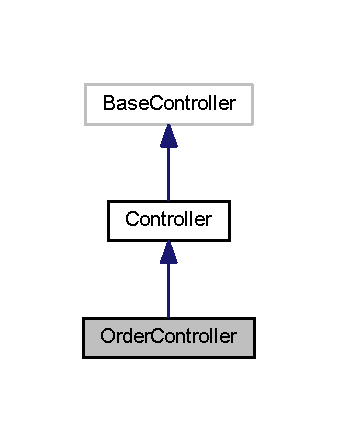
\includegraphics[width=162pt]{class_app_1_1_http_1_1_controllers_1_1_order_controller__coll__graph}
\end{center}
\end{figure}
\subsection*{Public Member Functions}
\begin{DoxyCompactItemize}
\item 
\mbox{\hyperlink{class_app_1_1_http_1_1_controllers_1_1_order_controller_a5b75ba6bc9debb999c0186a31978ec03}{\+\_\+\+\_\+construct}} (\$repository)
\item 
\mbox{\hyperlink{class_app_1_1_http_1_1_controllers_1_1_order_controller_a149eb92716c1084a935e04a8d95f7347}{index}} ()
\item 
\mbox{\hyperlink{class_app_1_1_http_1_1_controllers_1_1_order_controller_a4fa811c83f27da01b0d92bdb2a711a13}{create}} (\$request)
\item 
\mbox{\hyperlink{class_app_1_1_http_1_1_controllers_1_1_order_controller_ab7b27a90191560dcef32126b0945db0d}{update}} (\$request)
\item 
\mbox{\hyperlink{class_app_1_1_http_1_1_controllers_1_1_order_controller_a126a3799c44d72393ca4732081306dfd}{delete}} (\$request)
\end{DoxyCompactItemize}


\subsection{Detailed Description}
\mbox{\hyperlink{class_app_1_1_http_1_1_controllers_1_1_controller}{Controller}} for the orders. 

\subsection{Constructor \& Destructor Documentation}
\mbox{\Hypertarget{class_app_1_1_http_1_1_controllers_1_1_order_controller_a5b75ba6bc9debb999c0186a31978ec03}\label{class_app_1_1_http_1_1_controllers_1_1_order_controller_a5b75ba6bc9debb999c0186a31978ec03}} 
\index{App\+::\+Http\+::\+Controllers\+::\+Order\+Controller@{App\+::\+Http\+::\+Controllers\+::\+Order\+Controller}!\+\_\+\+\_\+construct@{\+\_\+\+\_\+construct}}
\index{\+\_\+\+\_\+construct@{\+\_\+\+\_\+construct}!App\+::\+Http\+::\+Controllers\+::\+Order\+Controller@{App\+::\+Http\+::\+Controllers\+::\+Order\+Controller}}
\subsubsection{\texorpdfstring{\+\_\+\+\_\+construct()}{\_\_construct()}}
{\footnotesize\ttfamily \+\_\+\+\_\+construct (\begin{DoxyParamCaption}\item[{}]{\$repository }\end{DoxyParamCaption})}

Using dependency injection to get the repository connected to the A\+PI in the app\+\_\+providers.


\begin{DoxyParams}[1]{Parameters}
interface & {\em \$repository} & \\
\hline
\end{DoxyParams}


\subsection{Member Function Documentation}
\mbox{\Hypertarget{class_app_1_1_http_1_1_controllers_1_1_order_controller_a4fa811c83f27da01b0d92bdb2a711a13}\label{class_app_1_1_http_1_1_controllers_1_1_order_controller_a4fa811c83f27da01b0d92bdb2a711a13}} 
\index{App\+::\+Http\+::\+Controllers\+::\+Order\+Controller@{App\+::\+Http\+::\+Controllers\+::\+Order\+Controller}!create@{create}}
\index{create@{create}!App\+::\+Http\+::\+Controllers\+::\+Order\+Controller@{App\+::\+Http\+::\+Controllers\+::\+Order\+Controller}}
\subsubsection{\texorpdfstring{create()}{create()}}
{\footnotesize\ttfamily create (\begin{DoxyParamCaption}\item[{}]{\$request }\end{DoxyParamCaption})}

Store a new order.

\begin{DoxyReturn}{Returns}
boolean 
\end{DoxyReturn}
\mbox{\Hypertarget{class_app_1_1_http_1_1_controllers_1_1_order_controller_a126a3799c44d72393ca4732081306dfd}\label{class_app_1_1_http_1_1_controllers_1_1_order_controller_a126a3799c44d72393ca4732081306dfd}} 
\index{App\+::\+Http\+::\+Controllers\+::\+Order\+Controller@{App\+::\+Http\+::\+Controllers\+::\+Order\+Controller}!delete@{delete}}
\index{delete@{delete}!App\+::\+Http\+::\+Controllers\+::\+Order\+Controller@{App\+::\+Http\+::\+Controllers\+::\+Order\+Controller}}
\subsubsection{\texorpdfstring{delete()}{delete()}}
{\footnotesize\ttfamily delete (\begin{DoxyParamCaption}\item[{}]{\$request }\end{DoxyParamCaption})}

Delete an order.

\begin{DoxyReturn}{Returns}
boolean 
\end{DoxyReturn}
\mbox{\Hypertarget{class_app_1_1_http_1_1_controllers_1_1_order_controller_a149eb92716c1084a935e04a8d95f7347}\label{class_app_1_1_http_1_1_controllers_1_1_order_controller_a149eb92716c1084a935e04a8d95f7347}} 
\index{App\+::\+Http\+::\+Controllers\+::\+Order\+Controller@{App\+::\+Http\+::\+Controllers\+::\+Order\+Controller}!index@{index}}
\index{index@{index}!App\+::\+Http\+::\+Controllers\+::\+Order\+Controller@{App\+::\+Http\+::\+Controllers\+::\+Order\+Controller}}
\subsubsection{\texorpdfstring{index()}{index()}}
{\footnotesize\ttfamily index (\begin{DoxyParamCaption}{ }\end{DoxyParamCaption})}

Returns all the orders.

\begin{DoxyReturn}{Returns}
array 
\end{DoxyReturn}
\mbox{\Hypertarget{class_app_1_1_http_1_1_controllers_1_1_order_controller_ab7b27a90191560dcef32126b0945db0d}\label{class_app_1_1_http_1_1_controllers_1_1_order_controller_ab7b27a90191560dcef32126b0945db0d}} 
\index{App\+::\+Http\+::\+Controllers\+::\+Order\+Controller@{App\+::\+Http\+::\+Controllers\+::\+Order\+Controller}!update@{update}}
\index{update@{update}!App\+::\+Http\+::\+Controllers\+::\+Order\+Controller@{App\+::\+Http\+::\+Controllers\+::\+Order\+Controller}}
\subsubsection{\texorpdfstring{update()}{update()}}
{\footnotesize\ttfamily update (\begin{DoxyParamCaption}\item[{}]{\$request }\end{DoxyParamCaption})}

Update an order.

\begin{DoxyReturn}{Returns}
boolean 
\end{DoxyReturn}


The documentation for this class was generated from the following file\+:\begin{DoxyCompactItemize}
\item 
app/\+Http/\+Controllers/Order\+Controller.\+php\end{DoxyCompactItemize}

\hypertarget{class_app_1_1_models_1_1_product_1_1_product}{}\section{Product Class Reference}
\label{class_app_1_1_models_1_1_product_1_1_product}\index{Product@{Product}}


Inheritance diagram for Product\+:
\nopagebreak
\begin{figure}[H]
\begin{center}
\leavevmode
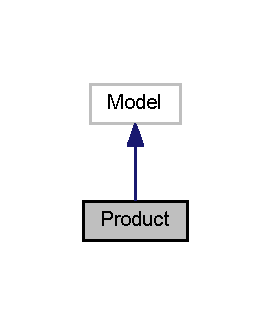
\includegraphics[width=130pt]{class_app_1_1_models_1_1_product_1_1_product__inherit__graph}
\end{center}
\end{figure}


Collaboration diagram for Product\+:
\nopagebreak
\begin{figure}[H]
\begin{center}
\leavevmode
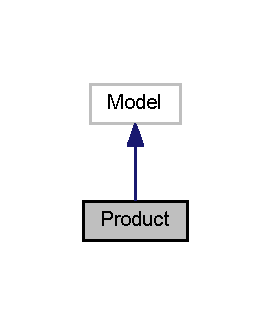
\includegraphics[width=130pt]{class_app_1_1_models_1_1_product_1_1_product__coll__graph}
\end{center}
\end{figure}
\subsection*{Public Member Functions}
\begin{DoxyCompactItemize}
\item 
\mbox{\hyperlink{class_app_1_1_models_1_1_product_1_1_product_a3ee17085a1e0dbe24e05f504147deb8a}{get\+Ingredients}} ()
\item 
\mbox{\hyperlink{class_app_1_1_models_1_1_product_1_1_product_a6f78a9ab9472f9f82fe70dd84d6c5e5c}{get\+Additionals}} ()
\item 
\mbox{\hyperlink{class_app_1_1_models_1_1_product_1_1_product_ada0bf69887885f455ebdfbe878e14543}{get\+Category}} ()
\item 
\mbox{\hyperlink{class_app_1_1_models_1_1_product_1_1_product_a4f44e7bc9de772c21b4304d11e87bf16}{get\+Group}} ()
\end{DoxyCompactItemize}
\subsection*{Protected Attributes}
\begin{DoxyCompactItemize}
\item 
\mbox{\Hypertarget{class_app_1_1_models_1_1_product_1_1_product_ae8876a14058f368335baccf35af4a22b}\label{class_app_1_1_models_1_1_product_1_1_product_ae8876a14058f368335baccf35af4a22b}} 
{\bfseries \$table} = \textquotesingle{}products\textquotesingle{}
\item 
{\bfseries \$fillabe}
\end{DoxyCompactItemize}


\subsection{Detailed Description}
Represents a product. This can be any food or drink. It\textquotesingle{}s connected to several classes\+: \mbox{\hyperlink{class_app_1_1_models_1_1_product_1_1_additional}{Additional}}, \mbox{\hyperlink{class_app_1_1_models_1_1_product_1_1_category}{Category}}, \mbox{\hyperlink{class_app_1_1_models_1_1_product_1_1_group}{Group}}, \mbox{\hyperlink{class_app_1_1_models_1_1_product_1_1_ingredient}{Ingredient}}

Accepts name\+: string, price\+: double, stock\+\_\+quantity\+: integer, category\+\_\+id\+: integer, group\+\_\+id\+: integer, status\+: tiny\+Integer. 

\subsection{Member Function Documentation}
\mbox{\Hypertarget{class_app_1_1_models_1_1_product_1_1_product_a6f78a9ab9472f9f82fe70dd84d6c5e5c}\label{class_app_1_1_models_1_1_product_1_1_product_a6f78a9ab9472f9f82fe70dd84d6c5e5c}} 
\index{App\+::\+Models\+::\+Product\+::\+Product@{App\+::\+Models\+::\+Product\+::\+Product}!get\+Additionals@{get\+Additionals}}
\index{get\+Additionals@{get\+Additionals}!App\+::\+Models\+::\+Product\+::\+Product@{App\+::\+Models\+::\+Product\+::\+Product}}
\subsubsection{\texorpdfstring{get\+Additionals()}{getAdditionals()}}
{\footnotesize\ttfamily get\+Additionals (\begin{DoxyParamCaption}{ }\end{DoxyParamCaption})}

Returns an array of additionals that can be attached to the product.

\begin{DoxyReturn}{Returns}
array 
\end{DoxyReturn}
\mbox{\Hypertarget{class_app_1_1_models_1_1_product_1_1_product_ada0bf69887885f455ebdfbe878e14543}\label{class_app_1_1_models_1_1_product_1_1_product_ada0bf69887885f455ebdfbe878e14543}} 
\index{App\+::\+Models\+::\+Product\+::\+Product@{App\+::\+Models\+::\+Product\+::\+Product}!get\+Category@{get\+Category}}
\index{get\+Category@{get\+Category}!App\+::\+Models\+::\+Product\+::\+Product@{App\+::\+Models\+::\+Product\+::\+Product}}
\subsubsection{\texorpdfstring{get\+Category()}{getCategory()}}
{\footnotesize\ttfamily get\+Category (\begin{DoxyParamCaption}{ }\end{DoxyParamCaption})}

Returns the \mbox{\hyperlink{class_app_1_1_models_1_1_product_1_1_category}{Category}} Object that this product belongs.

\begin{DoxyReturn}{Returns}
object 
\end{DoxyReturn}
\mbox{\Hypertarget{class_app_1_1_models_1_1_product_1_1_product_a4f44e7bc9de772c21b4304d11e87bf16}\label{class_app_1_1_models_1_1_product_1_1_product_a4f44e7bc9de772c21b4304d11e87bf16}} 
\index{App\+::\+Models\+::\+Product\+::\+Product@{App\+::\+Models\+::\+Product\+::\+Product}!get\+Group@{get\+Group}}
\index{get\+Group@{get\+Group}!App\+::\+Models\+::\+Product\+::\+Product@{App\+::\+Models\+::\+Product\+::\+Product}}
\subsubsection{\texorpdfstring{get\+Group()}{getGroup()}}
{\footnotesize\ttfamily get\+Group (\begin{DoxyParamCaption}{ }\end{DoxyParamCaption})}

Returns the \mbox{\hyperlink{class_app_1_1_models_1_1_product_1_1_group}{Group}} Object that this product belongs.

\begin{DoxyReturn}{Returns}
void 
\end{DoxyReturn}
\mbox{\Hypertarget{class_app_1_1_models_1_1_product_1_1_product_a3ee17085a1e0dbe24e05f504147deb8a}\label{class_app_1_1_models_1_1_product_1_1_product_a3ee17085a1e0dbe24e05f504147deb8a}} 
\index{App\+::\+Models\+::\+Product\+::\+Product@{App\+::\+Models\+::\+Product\+::\+Product}!get\+Ingredients@{get\+Ingredients}}
\index{get\+Ingredients@{get\+Ingredients}!App\+::\+Models\+::\+Product\+::\+Product@{App\+::\+Models\+::\+Product\+::\+Product}}
\subsubsection{\texorpdfstring{get\+Ingredients()}{getIngredients()}}
{\footnotesize\ttfamily get\+Ingredients (\begin{DoxyParamCaption}{ }\end{DoxyParamCaption})}

Returns an array of optionals ingredients for this product. Not all ingredients are stored in the database, just the ones that are optionals.

\begin{DoxyReturn}{Returns}
array 
\end{DoxyReturn}


\subsection{Field Documentation}
\mbox{\Hypertarget{class_app_1_1_models_1_1_product_1_1_product_ac5c29ce22e45a54200f88204e498d290}\label{class_app_1_1_models_1_1_product_1_1_product_ac5c29ce22e45a54200f88204e498d290}} 
\index{App\+::\+Models\+::\+Product\+::\+Product@{App\+::\+Models\+::\+Product\+::\+Product}!\$fillabe@{\$fillabe}}
\index{\$fillabe@{\$fillabe}!App\+::\+Models\+::\+Product\+::\+Product@{App\+::\+Models\+::\+Product\+::\+Product}}
\subsubsection{\texorpdfstring{\$fillabe}{$fillabe}}
{\footnotesize\ttfamily \$fillabe\hspace{0.3cm}{\ttfamily [protected]}}

{\bfseries Initial value\+:}
\begin{DoxyCode}
= [
        \textcolor{stringliteral}{'name'},
        \textcolor{stringliteral}{'price'},
        \textcolor{stringliteral}{'stock\_quantity'},
        \textcolor{stringliteral}{'category\_id'},
        \textcolor{stringliteral}{'group\_id'},
        \textcolor{stringliteral}{'status'}
    ]
\end{DoxyCode}


The documentation for this class was generated from the following file\+:\begin{DoxyCompactItemize}
\item 
app/\+Models/\+Product/Product.\+php\end{DoxyCompactItemize}

\hypertarget{class_app_1_1_http_1_1_controllers_1_1_product_1_1_product_controller}{}\section{Product\+Controller Class Reference}
\label{class_app_1_1_http_1_1_controllers_1_1_product_1_1_product_controller}\index{Product\+Controller@{Product\+Controller}}


Inheritance diagram for Product\+Controller\+:
\nopagebreak
\begin{figure}[H]
\begin{center}
\leavevmode
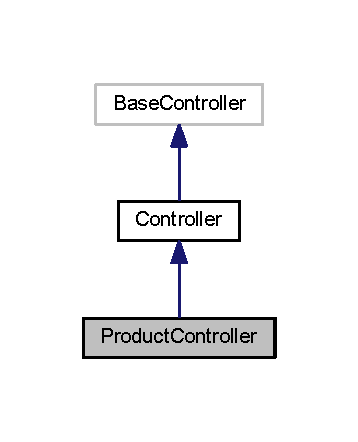
\includegraphics[width=172pt]{class_app_1_1_http_1_1_controllers_1_1_product_1_1_product_controller__inherit__graph}
\end{center}
\end{figure}


Collaboration diagram for Product\+Controller\+:
\nopagebreak
\begin{figure}[H]
\begin{center}
\leavevmode
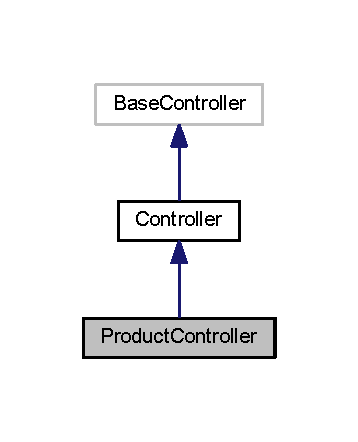
\includegraphics[width=172pt]{class_app_1_1_http_1_1_controllers_1_1_product_1_1_product_controller__coll__graph}
\end{center}
\end{figure}
\subsection*{Public Member Functions}
\begin{DoxyCompactItemize}
\item 
\mbox{\hyperlink{class_app_1_1_http_1_1_controllers_1_1_product_1_1_product_controller_a5b75ba6bc9debb999c0186a31978ec03}{\+\_\+\+\_\+construct}} (\$repository)
\item 
\mbox{\hyperlink{class_app_1_1_http_1_1_controllers_1_1_product_1_1_product_controller_af9d14e4ae6227970ad603987781573ca}{all}} ()
\item 
\mbox{\hyperlink{class_app_1_1_http_1_1_controllers_1_1_product_1_1_product_controller_a50e3bfb586b2f42932a6a93f3fbb0828}{get}} (\$id)
\item 
\mbox{\hyperlink{class_app_1_1_http_1_1_controllers_1_1_product_1_1_product_controller_a4fa811c83f27da01b0d92bdb2a711a13}{create}} (\$request)
\item 
\mbox{\hyperlink{class_app_1_1_http_1_1_controllers_1_1_product_1_1_product_controller_ab7b27a90191560dcef32126b0945db0d}{update}} (\$request)
\item 
\mbox{\hyperlink{class_app_1_1_http_1_1_controllers_1_1_product_1_1_product_controller_a126a3799c44d72393ca4732081306dfd}{delete}} (\$request)
\end{DoxyCompactItemize}


\subsection{Detailed Description}
\mbox{\hyperlink{class_app_1_1_http_1_1_controllers_1_1_controller}{Controller}} for the products. 

\subsection{Constructor \& Destructor Documentation}
\mbox{\Hypertarget{class_app_1_1_http_1_1_controllers_1_1_product_1_1_product_controller_a5b75ba6bc9debb999c0186a31978ec03}\label{class_app_1_1_http_1_1_controllers_1_1_product_1_1_product_controller_a5b75ba6bc9debb999c0186a31978ec03}} 
\index{App\+::\+Http\+::\+Controllers\+::\+Product\+::\+Product\+Controller@{App\+::\+Http\+::\+Controllers\+::\+Product\+::\+Product\+Controller}!\+\_\+\+\_\+construct@{\+\_\+\+\_\+construct}}
\index{\+\_\+\+\_\+construct@{\+\_\+\+\_\+construct}!App\+::\+Http\+::\+Controllers\+::\+Product\+::\+Product\+Controller@{App\+::\+Http\+::\+Controllers\+::\+Product\+::\+Product\+Controller}}
\subsubsection{\texorpdfstring{\+\_\+\+\_\+construct()}{\_\_construct()}}
{\footnotesize\ttfamily \+\_\+\+\_\+construct (\begin{DoxyParamCaption}\item[{}]{\$repository }\end{DoxyParamCaption})}

Using dependency injection to get the repository connected to the A\+PI in the app\+\_\+providers.


\begin{DoxyParams}[1]{Parameters}
interface & {\em \$repository} & \\
\hline
\end{DoxyParams}


\subsection{Member Function Documentation}
\mbox{\Hypertarget{class_app_1_1_http_1_1_controllers_1_1_product_1_1_product_controller_af9d14e4ae6227970ad603987781573ca}\label{class_app_1_1_http_1_1_controllers_1_1_product_1_1_product_controller_af9d14e4ae6227970ad603987781573ca}} 
\index{App\+::\+Http\+::\+Controllers\+::\+Product\+::\+Product\+Controller@{App\+::\+Http\+::\+Controllers\+::\+Product\+::\+Product\+Controller}!all@{all}}
\index{all@{all}!App\+::\+Http\+::\+Controllers\+::\+Product\+::\+Product\+Controller@{App\+::\+Http\+::\+Controllers\+::\+Product\+::\+Product\+Controller}}
\subsubsection{\texorpdfstring{all()}{all()}}
{\footnotesize\ttfamily all (\begin{DoxyParamCaption}{ }\end{DoxyParamCaption})}

Returns an array of Product objects.

\begin{DoxyReturn}{Returns}
array 
\end{DoxyReturn}
\mbox{\Hypertarget{class_app_1_1_http_1_1_controllers_1_1_product_1_1_product_controller_a4fa811c83f27da01b0d92bdb2a711a13}\label{class_app_1_1_http_1_1_controllers_1_1_product_1_1_product_controller_a4fa811c83f27da01b0d92bdb2a711a13}} 
\index{App\+::\+Http\+::\+Controllers\+::\+Product\+::\+Product\+Controller@{App\+::\+Http\+::\+Controllers\+::\+Product\+::\+Product\+Controller}!create@{create}}
\index{create@{create}!App\+::\+Http\+::\+Controllers\+::\+Product\+::\+Product\+Controller@{App\+::\+Http\+::\+Controllers\+::\+Product\+::\+Product\+Controller}}
\subsubsection{\texorpdfstring{create()}{create()}}
{\footnotesize\ttfamily create (\begin{DoxyParamCaption}\item[{}]{\$request }\end{DoxyParamCaption})}

Store a new product.

\begin{DoxyReturn}{Returns}
boolean 
\end{DoxyReturn}
\mbox{\Hypertarget{class_app_1_1_http_1_1_controllers_1_1_product_1_1_product_controller_a126a3799c44d72393ca4732081306dfd}\label{class_app_1_1_http_1_1_controllers_1_1_product_1_1_product_controller_a126a3799c44d72393ca4732081306dfd}} 
\index{App\+::\+Http\+::\+Controllers\+::\+Product\+::\+Product\+Controller@{App\+::\+Http\+::\+Controllers\+::\+Product\+::\+Product\+Controller}!delete@{delete}}
\index{delete@{delete}!App\+::\+Http\+::\+Controllers\+::\+Product\+::\+Product\+Controller@{App\+::\+Http\+::\+Controllers\+::\+Product\+::\+Product\+Controller}}
\subsubsection{\texorpdfstring{delete()}{delete()}}
{\footnotesize\ttfamily delete (\begin{DoxyParamCaption}\item[{}]{\$request }\end{DoxyParamCaption})}

Delete a product.

\begin{DoxyReturn}{Returns}
boolean 
\end{DoxyReturn}
\mbox{\Hypertarget{class_app_1_1_http_1_1_controllers_1_1_product_1_1_product_controller_a50e3bfb586b2f42932a6a93f3fbb0828}\label{class_app_1_1_http_1_1_controllers_1_1_product_1_1_product_controller_a50e3bfb586b2f42932a6a93f3fbb0828}} 
\index{App\+::\+Http\+::\+Controllers\+::\+Product\+::\+Product\+Controller@{App\+::\+Http\+::\+Controllers\+::\+Product\+::\+Product\+Controller}!get@{get}}
\index{get@{get}!App\+::\+Http\+::\+Controllers\+::\+Product\+::\+Product\+Controller@{App\+::\+Http\+::\+Controllers\+::\+Product\+::\+Product\+Controller}}
\subsubsection{\texorpdfstring{get()}{get()}}
{\footnotesize\ttfamily get (\begin{DoxyParamCaption}\item[{}]{\$id }\end{DoxyParamCaption})}

Returns an Product Object with the provided id.

\begin{DoxyReturn}{Returns}
object 
\end{DoxyReturn}
\mbox{\Hypertarget{class_app_1_1_http_1_1_controllers_1_1_product_1_1_product_controller_ab7b27a90191560dcef32126b0945db0d}\label{class_app_1_1_http_1_1_controllers_1_1_product_1_1_product_controller_ab7b27a90191560dcef32126b0945db0d}} 
\index{App\+::\+Http\+::\+Controllers\+::\+Product\+::\+Product\+Controller@{App\+::\+Http\+::\+Controllers\+::\+Product\+::\+Product\+Controller}!update@{update}}
\index{update@{update}!App\+::\+Http\+::\+Controllers\+::\+Product\+::\+Product\+Controller@{App\+::\+Http\+::\+Controllers\+::\+Product\+::\+Product\+Controller}}
\subsubsection{\texorpdfstring{update()}{update()}}
{\footnotesize\ttfamily update (\begin{DoxyParamCaption}\item[{}]{\$request }\end{DoxyParamCaption})}

Update a product.

\begin{DoxyReturn}{Returns}
boolean 
\end{DoxyReturn}


The documentation for this class was generated from the following file\+:\begin{DoxyCompactItemize}
\item 
app/\+Http/\+Controllers/\+Product/Product\+Controller.\+php\end{DoxyCompactItemize}

\hypertarget{interface_app_1_1_repositories_1_1_product_1_1_product_repository_interface}{}\section{Product\+Repository\+Interface Interface Reference}
\label{interface_app_1_1_repositories_1_1_product_1_1_product_repository_interface}\index{Product\+Repository\+Interface@{Product\+Repository\+Interface}}
\subsection*{Public Member Functions}
\begin{DoxyCompactItemize}
\item 
\mbox{\hyperlink{interface_app_1_1_repositories_1_1_product_1_1_product_repository_interface_af9d14e4ae6227970ad603987781573ca}{all}} ()
\item 
\mbox{\hyperlink{interface_app_1_1_repositories_1_1_product_1_1_product_repository_interface_a50e3bfb586b2f42932a6a93f3fbb0828}{get}} (\$id)
\item 
\mbox{\hyperlink{interface_app_1_1_repositories_1_1_product_1_1_product_repository_interface_a4fa811c83f27da01b0d92bdb2a711a13}{create}} (\$request)
\item 
\mbox{\hyperlink{interface_app_1_1_repositories_1_1_product_1_1_product_repository_interface_a2aedea52c52e54ba3c4c9f60423e7ef1}{udpate}} (\$request)
\item 
\mbox{\hyperlink{interface_app_1_1_repositories_1_1_product_1_1_product_repository_interface_a126a3799c44d72393ca4732081306dfd}{delete}} (\$request)
\end{DoxyCompactItemize}


\subsection{Detailed Description}
Interface for the Product\+Repository 

\subsection{Member Function Documentation}
\mbox{\Hypertarget{interface_app_1_1_repositories_1_1_product_1_1_product_repository_interface_af9d14e4ae6227970ad603987781573ca}\label{interface_app_1_1_repositories_1_1_product_1_1_product_repository_interface_af9d14e4ae6227970ad603987781573ca}} 
\index{App\+::\+Repositories\+::\+Product\+::\+Product\+Repository\+Interface@{App\+::\+Repositories\+::\+Product\+::\+Product\+Repository\+Interface}!all@{all}}
\index{all@{all}!App\+::\+Repositories\+::\+Product\+::\+Product\+Repository\+Interface@{App\+::\+Repositories\+::\+Product\+::\+Product\+Repository\+Interface}}
\subsubsection{\texorpdfstring{all()}{all()}}
{\footnotesize\ttfamily all (\begin{DoxyParamCaption}{ }\end{DoxyParamCaption})}

Returns an array of Product objects.

\begin{DoxyReturn}{Returns}
array 
\end{DoxyReturn}
\mbox{\Hypertarget{interface_app_1_1_repositories_1_1_product_1_1_product_repository_interface_a4fa811c83f27da01b0d92bdb2a711a13}\label{interface_app_1_1_repositories_1_1_product_1_1_product_repository_interface_a4fa811c83f27da01b0d92bdb2a711a13}} 
\index{App\+::\+Repositories\+::\+Product\+::\+Product\+Repository\+Interface@{App\+::\+Repositories\+::\+Product\+::\+Product\+Repository\+Interface}!create@{create}}
\index{create@{create}!App\+::\+Repositories\+::\+Product\+::\+Product\+Repository\+Interface@{App\+::\+Repositories\+::\+Product\+::\+Product\+Repository\+Interface}}
\subsubsection{\texorpdfstring{create()}{create()}}
{\footnotesize\ttfamily create (\begin{DoxyParamCaption}\item[{}]{\$request }\end{DoxyParamCaption})}

Returns a boolean reflecting the creation status.

\begin{DoxyReturn}{Returns}
boolean 
\end{DoxyReturn}
\mbox{\Hypertarget{interface_app_1_1_repositories_1_1_product_1_1_product_repository_interface_a126a3799c44d72393ca4732081306dfd}\label{interface_app_1_1_repositories_1_1_product_1_1_product_repository_interface_a126a3799c44d72393ca4732081306dfd}} 
\index{App\+::\+Repositories\+::\+Product\+::\+Product\+Repository\+Interface@{App\+::\+Repositories\+::\+Product\+::\+Product\+Repository\+Interface}!delete@{delete}}
\index{delete@{delete}!App\+::\+Repositories\+::\+Product\+::\+Product\+Repository\+Interface@{App\+::\+Repositories\+::\+Product\+::\+Product\+Repository\+Interface}}
\subsubsection{\texorpdfstring{delete()}{delete()}}
{\footnotesize\ttfamily delete (\begin{DoxyParamCaption}\item[{}]{\$request }\end{DoxyParamCaption})}

Returns a boolean reflecting the deletion status.

\begin{DoxyReturn}{Returns}
boolean 
\end{DoxyReturn}
\mbox{\Hypertarget{interface_app_1_1_repositories_1_1_product_1_1_product_repository_interface_a50e3bfb586b2f42932a6a93f3fbb0828}\label{interface_app_1_1_repositories_1_1_product_1_1_product_repository_interface_a50e3bfb586b2f42932a6a93f3fbb0828}} 
\index{App\+::\+Repositories\+::\+Product\+::\+Product\+Repository\+Interface@{App\+::\+Repositories\+::\+Product\+::\+Product\+Repository\+Interface}!get@{get}}
\index{get@{get}!App\+::\+Repositories\+::\+Product\+::\+Product\+Repository\+Interface@{App\+::\+Repositories\+::\+Product\+::\+Product\+Repository\+Interface}}
\subsubsection{\texorpdfstring{get()}{get()}}
{\footnotesize\ttfamily get (\begin{DoxyParamCaption}\item[{}]{\$id }\end{DoxyParamCaption})}

Returns an Product Object with the provided id.

\begin{DoxyReturn}{Returns}
object 
\end{DoxyReturn}
\mbox{\Hypertarget{interface_app_1_1_repositories_1_1_product_1_1_product_repository_interface_a2aedea52c52e54ba3c4c9f60423e7ef1}\label{interface_app_1_1_repositories_1_1_product_1_1_product_repository_interface_a2aedea52c52e54ba3c4c9f60423e7ef1}} 
\index{App\+::\+Repositories\+::\+Product\+::\+Product\+Repository\+Interface@{App\+::\+Repositories\+::\+Product\+::\+Product\+Repository\+Interface}!udpate@{udpate}}
\index{udpate@{udpate}!App\+::\+Repositories\+::\+Product\+::\+Product\+Repository\+Interface@{App\+::\+Repositories\+::\+Product\+::\+Product\+Repository\+Interface}}
\subsubsection{\texorpdfstring{udpate()}{udpate()}}
{\footnotesize\ttfamily udpate (\begin{DoxyParamCaption}\item[{}]{\$request }\end{DoxyParamCaption})}

Returns a boolean reflecting the update status.

\begin{DoxyReturn}{Returns}
boolean 
\end{DoxyReturn}


The documentation for this interface was generated from the following file\+:\begin{DoxyCompactItemize}
\item 
app/\+Repositories/\+Product/Product\+Repository\+Interface.\+php\end{DoxyCompactItemize}

\hypertarget{class_app_1_1_models_1_1_table}{}\section{Table Class Reference}
\label{class_app_1_1_models_1_1_table}\index{Table@{Table}}


Inheritance diagram for Table\+:
\nopagebreak
\begin{figure}[H]
\begin{center}
\leavevmode
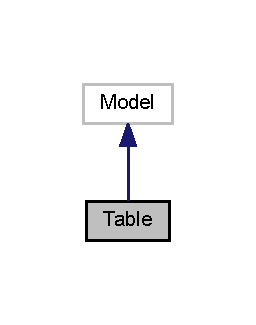
\includegraphics[width=123pt]{class_app_1_1_models_1_1_table__inherit__graph}
\end{center}
\end{figure}


Collaboration diagram for Table\+:
\nopagebreak
\begin{figure}[H]
\begin{center}
\leavevmode
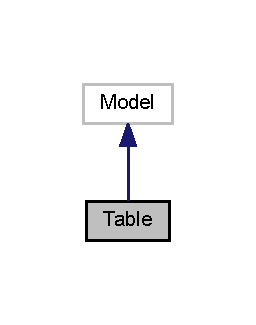
\includegraphics[width=123pt]{class_app_1_1_models_1_1_table__coll__graph}
\end{center}
\end{figure}
\subsection*{Protected Attributes}
\begin{DoxyCompactItemize}
\item 
\mbox{\Hypertarget{class_app_1_1_models_1_1_table_ae8876a14058f368335baccf35af4a22b}\label{class_app_1_1_models_1_1_table_ae8876a14058f368335baccf35af4a22b}} 
{\bfseries \$table} = \textquotesingle{}tables\textquotesingle{}
\item 
{\bfseries \$fillabe}
\end{DoxyCompactItemize}


\subsection{Detailed Description}
Represents a table (a physical table, where the clients sit, not a database one).

Accepts name\+: string, status\+: tiny\+Integer. Status represents if the \mbox{\hyperlink{class_app_1_1_models_1_1_table}{Table}} is available or not. 

\subsection{Field Documentation}
\mbox{\Hypertarget{class_app_1_1_models_1_1_table_ac5c29ce22e45a54200f88204e498d290}\label{class_app_1_1_models_1_1_table_ac5c29ce22e45a54200f88204e498d290}} 
\index{App\+::\+Models\+::\+Table@{App\+::\+Models\+::\+Table}!\$fillabe@{\$fillabe}}
\index{\$fillabe@{\$fillabe}!App\+::\+Models\+::\+Table@{App\+::\+Models\+::\+Table}}
\subsubsection{\texorpdfstring{\$fillabe}{$fillabe}}
{\footnotesize\ttfamily \$fillabe\hspace{0.3cm}{\ttfamily [protected]}}

{\bfseries Initial value\+:}
\begin{DoxyCode}
= [
        \textcolor{stringliteral}{'name'},
        \textcolor{stringliteral}{'status'}
    ]
\end{DoxyCode}


The documentation for this class was generated from the following file\+:\begin{DoxyCompactItemize}
\item 
app/\+Models/Table.\+php\end{DoxyCompactItemize}

\hypertarget{class_app_1_1_http_1_1_controllers_1_1_table_controller}{}\section{Table\+Controller Class Reference}
\label{class_app_1_1_http_1_1_controllers_1_1_table_controller}\index{Table\+Controller@{Table\+Controller}}


Inheritance diagram for Table\+Controller\+:
\nopagebreak
\begin{figure}[H]
\begin{center}
\leavevmode
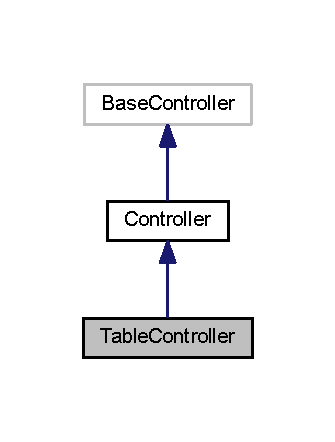
\includegraphics[width=161pt]{class_app_1_1_http_1_1_controllers_1_1_table_controller__inherit__graph}
\end{center}
\end{figure}


Collaboration diagram for Table\+Controller\+:
\nopagebreak
\begin{figure}[H]
\begin{center}
\leavevmode
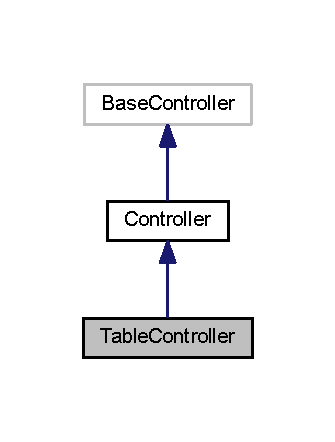
\includegraphics[width=161pt]{class_app_1_1_http_1_1_controllers_1_1_table_controller__coll__graph}
\end{center}
\end{figure}
\subsection*{Public Member Functions}
\begin{DoxyCompactItemize}
\item 
\mbox{\hyperlink{class_app_1_1_http_1_1_controllers_1_1_table_controller_a5b75ba6bc9debb999c0186a31978ec03}{\+\_\+\+\_\+construct}} (\$repository)
\item 
\mbox{\hyperlink{class_app_1_1_http_1_1_controllers_1_1_table_controller_a149eb92716c1084a935e04a8d95f7347}{index}} ()
\item 
\mbox{\hyperlink{class_app_1_1_http_1_1_controllers_1_1_table_controller_a4fa811c83f27da01b0d92bdb2a711a13}{create}} (\$request)
\item 
\mbox{\hyperlink{class_app_1_1_http_1_1_controllers_1_1_table_controller_ab7b27a90191560dcef32126b0945db0d}{update}} (\$request)
\item 
\mbox{\hyperlink{class_app_1_1_http_1_1_controllers_1_1_table_controller_a126a3799c44d72393ca4732081306dfd}{delete}} (\$request)
\end{DoxyCompactItemize}


\subsection{Detailed Description}
\mbox{\hyperlink{class_app_1_1_http_1_1_controllers_1_1_controller}{Controller}} for the tables. 

\subsection{Constructor \& Destructor Documentation}
\mbox{\Hypertarget{class_app_1_1_http_1_1_controllers_1_1_table_controller_a5b75ba6bc9debb999c0186a31978ec03}\label{class_app_1_1_http_1_1_controllers_1_1_table_controller_a5b75ba6bc9debb999c0186a31978ec03}} 
\index{App\+::\+Http\+::\+Controllers\+::\+Table\+Controller@{App\+::\+Http\+::\+Controllers\+::\+Table\+Controller}!\+\_\+\+\_\+construct@{\+\_\+\+\_\+construct}}
\index{\+\_\+\+\_\+construct@{\+\_\+\+\_\+construct}!App\+::\+Http\+::\+Controllers\+::\+Table\+Controller@{App\+::\+Http\+::\+Controllers\+::\+Table\+Controller}}
\subsubsection{\texorpdfstring{\+\_\+\+\_\+construct()}{\_\_construct()}}
{\footnotesize\ttfamily \+\_\+\+\_\+construct (\begin{DoxyParamCaption}\item[{}]{\$repository }\end{DoxyParamCaption})}

Using dependency injection to get the repository connected to the A\+PI in the app\+\_\+providers.


\begin{DoxyParams}[1]{Parameters}
interface & {\em \$repository} & \\
\hline
\end{DoxyParams}


\subsection{Member Function Documentation}
\mbox{\Hypertarget{class_app_1_1_http_1_1_controllers_1_1_table_controller_a4fa811c83f27da01b0d92bdb2a711a13}\label{class_app_1_1_http_1_1_controllers_1_1_table_controller_a4fa811c83f27da01b0d92bdb2a711a13}} 
\index{App\+::\+Http\+::\+Controllers\+::\+Table\+Controller@{App\+::\+Http\+::\+Controllers\+::\+Table\+Controller}!create@{create}}
\index{create@{create}!App\+::\+Http\+::\+Controllers\+::\+Table\+Controller@{App\+::\+Http\+::\+Controllers\+::\+Table\+Controller}}
\subsubsection{\texorpdfstring{create()}{create()}}
{\footnotesize\ttfamily create (\begin{DoxyParamCaption}\item[{}]{\$request }\end{DoxyParamCaption})}

Store a new table.

\begin{DoxyReturn}{Returns}
boolean 
\end{DoxyReturn}
\mbox{\Hypertarget{class_app_1_1_http_1_1_controllers_1_1_table_controller_a126a3799c44d72393ca4732081306dfd}\label{class_app_1_1_http_1_1_controllers_1_1_table_controller_a126a3799c44d72393ca4732081306dfd}} 
\index{App\+::\+Http\+::\+Controllers\+::\+Table\+Controller@{App\+::\+Http\+::\+Controllers\+::\+Table\+Controller}!delete@{delete}}
\index{delete@{delete}!App\+::\+Http\+::\+Controllers\+::\+Table\+Controller@{App\+::\+Http\+::\+Controllers\+::\+Table\+Controller}}
\subsubsection{\texorpdfstring{delete()}{delete()}}
{\footnotesize\ttfamily delete (\begin{DoxyParamCaption}\item[{}]{\$request }\end{DoxyParamCaption})}

Delete a table.

\begin{DoxyReturn}{Returns}
boolean 
\end{DoxyReturn}
\mbox{\Hypertarget{class_app_1_1_http_1_1_controllers_1_1_table_controller_a149eb92716c1084a935e04a8d95f7347}\label{class_app_1_1_http_1_1_controllers_1_1_table_controller_a149eb92716c1084a935e04a8d95f7347}} 
\index{App\+::\+Http\+::\+Controllers\+::\+Table\+Controller@{App\+::\+Http\+::\+Controllers\+::\+Table\+Controller}!index@{index}}
\index{index@{index}!App\+::\+Http\+::\+Controllers\+::\+Table\+Controller@{App\+::\+Http\+::\+Controllers\+::\+Table\+Controller}}
\subsubsection{\texorpdfstring{index()}{index()}}
{\footnotesize\ttfamily index (\begin{DoxyParamCaption}{ }\end{DoxyParamCaption})}

Returns all the tables.

\begin{DoxyReturn}{Returns}
array 
\end{DoxyReturn}
\mbox{\Hypertarget{class_app_1_1_http_1_1_controllers_1_1_table_controller_ab7b27a90191560dcef32126b0945db0d}\label{class_app_1_1_http_1_1_controllers_1_1_table_controller_ab7b27a90191560dcef32126b0945db0d}} 
\index{App\+::\+Http\+::\+Controllers\+::\+Table\+Controller@{App\+::\+Http\+::\+Controllers\+::\+Table\+Controller}!update@{update}}
\index{update@{update}!App\+::\+Http\+::\+Controllers\+::\+Table\+Controller@{App\+::\+Http\+::\+Controllers\+::\+Table\+Controller}}
\subsubsection{\texorpdfstring{update()}{update()}}
{\footnotesize\ttfamily update (\begin{DoxyParamCaption}\item[{}]{\$request }\end{DoxyParamCaption})}

Update a table.

\begin{DoxyReturn}{Returns}
boolean 
\end{DoxyReturn}


The documentation for this class was generated from the following file\+:\begin{DoxyCompactItemize}
\item 
app/\+Http/\+Controllers/Table\+Controller.\+php\end{DoxyCompactItemize}

\hypertarget{class_app_1_1_models_1_1_user}{}\section{User Class Reference}
\label{class_app_1_1_models_1_1_user}\index{User@{User}}


Inheritance diagram for User\+:
\nopagebreak
\begin{figure}[H]
\begin{center}
\leavevmode
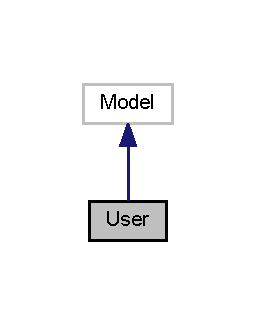
\includegraphics[width=123pt]{class_app_1_1_models_1_1_user__inherit__graph}
\end{center}
\end{figure}


Collaboration diagram for User\+:
\nopagebreak
\begin{figure}[H]
\begin{center}
\leavevmode
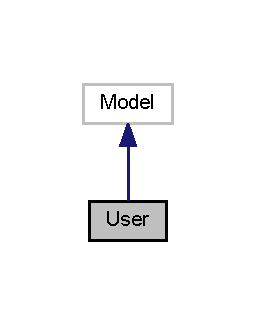
\includegraphics[width=123pt]{class_app_1_1_models_1_1_user__coll__graph}
\end{center}
\end{figure}
\subsection*{Protected Attributes}
\begin{DoxyCompactItemize}
\item 
\mbox{\Hypertarget{class_app_1_1_models_1_1_user_ae8876a14058f368335baccf35af4a22b}\label{class_app_1_1_models_1_1_user_ae8876a14058f368335baccf35af4a22b}} 
{\bfseries \$table} = \textquotesingle{}users\textquotesingle{}
\item 
{\bfseries \$fillabe}
\item 
\mbox{\Hypertarget{class_app_1_1_models_1_1_user_a4a374564d2858d8ae869a8fb890aad56}\label{class_app_1_1_models_1_1_user_a4a374564d2858d8ae869a8fb890aad56}} 
{\bfseries \$hidden} = \mbox{[}\textquotesingle{}password\textquotesingle{}\mbox{]}
\end{DoxyCompactItemize}


\subsection{Detailed Description}
Represents a user. This user has access to the list of orders. This user has access to the /admin if is\+Admin is 1. A waiter is not stored as a user!

Accepts name\+: string, email\+: string, password\+: string, is\+Admin\+: tiny\+Integer, status\+: tiny\+Integer. Status represents if the user is active or not. If not, logging will always fail. The password is a hidden field, so it\textquotesingle{}ll not be passed along when getting the full object. 

\subsection{Field Documentation}
\mbox{\Hypertarget{class_app_1_1_models_1_1_user_ac5c29ce22e45a54200f88204e498d290}\label{class_app_1_1_models_1_1_user_ac5c29ce22e45a54200f88204e498d290}} 
\index{App\+::\+Models\+::\+User@{App\+::\+Models\+::\+User}!\$fillabe@{\$fillabe}}
\index{\$fillabe@{\$fillabe}!App\+::\+Models\+::\+User@{App\+::\+Models\+::\+User}}
\subsubsection{\texorpdfstring{\$fillabe}{$fillabe}}
{\footnotesize\ttfamily \$fillabe\hspace{0.3cm}{\ttfamily [protected]}}

{\bfseries Initial value\+:}
\begin{DoxyCode}
= [
        \textcolor{stringliteral}{'name'},
        \textcolor{stringliteral}{'email'},
        \textcolor{stringliteral}{'password'},
        \textcolor{stringliteral}{'isAdmin'},
        \textcolor{stringliteral}{'status'}
    ]
\end{DoxyCode}


The documentation for this class was generated from the following file\+:\begin{DoxyCompactItemize}
\item 
app/\+Models/User.\+php\end{DoxyCompactItemize}

\hypertarget{class_app_1_1_http_1_1_controllers_1_1_user_controller}{}\section{User\+Controller Class Reference}
\label{class_app_1_1_http_1_1_controllers_1_1_user_controller}\index{User\+Controller@{User\+Controller}}


Inheritance diagram for User\+Controller\+:
\nopagebreak
\begin{figure}[H]
\begin{center}
\leavevmode
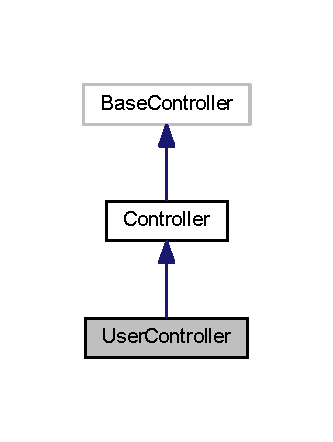
\includegraphics[width=160pt]{class_app_1_1_http_1_1_controllers_1_1_user_controller__inherit__graph}
\end{center}
\end{figure}


Collaboration diagram for User\+Controller\+:
\nopagebreak
\begin{figure}[H]
\begin{center}
\leavevmode
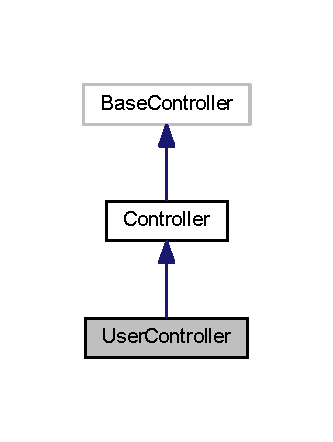
\includegraphics[width=160pt]{class_app_1_1_http_1_1_controllers_1_1_user_controller__coll__graph}
\end{center}
\end{figure}
\subsection*{Public Member Functions}
\begin{DoxyCompactItemize}
\item 
\mbox{\hyperlink{class_app_1_1_http_1_1_controllers_1_1_user_controller_a5b75ba6bc9debb999c0186a31978ec03}{\+\_\+\+\_\+construct}} (\$repository)
\item 
\mbox{\hyperlink{class_app_1_1_http_1_1_controllers_1_1_user_controller_a149eb92716c1084a935e04a8d95f7347}{index}} ()
\item 
\mbox{\hyperlink{class_app_1_1_http_1_1_controllers_1_1_user_controller_a4fa811c83f27da01b0d92bdb2a711a13}{create}} (\$request)
\item 
\mbox{\hyperlink{class_app_1_1_http_1_1_controllers_1_1_user_controller_ab7b27a90191560dcef32126b0945db0d}{update}} (\$request)
\item 
\mbox{\hyperlink{class_app_1_1_http_1_1_controllers_1_1_user_controller_a126a3799c44d72393ca4732081306dfd}{delete}} (\$request)
\end{DoxyCompactItemize}


\subsection{Detailed Description}
\mbox{\hyperlink{class_app_1_1_http_1_1_controllers_1_1_controller}{Controller}} for the users. 

\subsection{Constructor \& Destructor Documentation}
\mbox{\Hypertarget{class_app_1_1_http_1_1_controllers_1_1_user_controller_a5b75ba6bc9debb999c0186a31978ec03}\label{class_app_1_1_http_1_1_controllers_1_1_user_controller_a5b75ba6bc9debb999c0186a31978ec03}} 
\index{App\+::\+Http\+::\+Controllers\+::\+User\+Controller@{App\+::\+Http\+::\+Controllers\+::\+User\+Controller}!\+\_\+\+\_\+construct@{\+\_\+\+\_\+construct}}
\index{\+\_\+\+\_\+construct@{\+\_\+\+\_\+construct}!App\+::\+Http\+::\+Controllers\+::\+User\+Controller@{App\+::\+Http\+::\+Controllers\+::\+User\+Controller}}
\subsubsection{\texorpdfstring{\+\_\+\+\_\+construct()}{\_\_construct()}}
{\footnotesize\ttfamily \+\_\+\+\_\+construct (\begin{DoxyParamCaption}\item[{}]{\$repository }\end{DoxyParamCaption})}

Using dependency injection to get the repository connected to the A\+PI in the app\+\_\+providers.


\begin{DoxyParams}[1]{Parameters}
interface & {\em \$repository} & \\
\hline
\end{DoxyParams}


\subsection{Member Function Documentation}
\mbox{\Hypertarget{class_app_1_1_http_1_1_controllers_1_1_user_controller_a4fa811c83f27da01b0d92bdb2a711a13}\label{class_app_1_1_http_1_1_controllers_1_1_user_controller_a4fa811c83f27da01b0d92bdb2a711a13}} 
\index{App\+::\+Http\+::\+Controllers\+::\+User\+Controller@{App\+::\+Http\+::\+Controllers\+::\+User\+Controller}!create@{create}}
\index{create@{create}!App\+::\+Http\+::\+Controllers\+::\+User\+Controller@{App\+::\+Http\+::\+Controllers\+::\+User\+Controller}}
\subsubsection{\texorpdfstring{create()}{create()}}
{\footnotesize\ttfamily create (\begin{DoxyParamCaption}\item[{}]{\$request }\end{DoxyParamCaption})}

Store a new user.

\begin{DoxyReturn}{Returns}
boolean 
\end{DoxyReturn}
\mbox{\Hypertarget{class_app_1_1_http_1_1_controllers_1_1_user_controller_a126a3799c44d72393ca4732081306dfd}\label{class_app_1_1_http_1_1_controllers_1_1_user_controller_a126a3799c44d72393ca4732081306dfd}} 
\index{App\+::\+Http\+::\+Controllers\+::\+User\+Controller@{App\+::\+Http\+::\+Controllers\+::\+User\+Controller}!delete@{delete}}
\index{delete@{delete}!App\+::\+Http\+::\+Controllers\+::\+User\+Controller@{App\+::\+Http\+::\+Controllers\+::\+User\+Controller}}
\subsubsection{\texorpdfstring{delete()}{delete()}}
{\footnotesize\ttfamily delete (\begin{DoxyParamCaption}\item[{}]{\$request }\end{DoxyParamCaption})}

Delete an user.

\begin{DoxyReturn}{Returns}
boolean 
\end{DoxyReturn}
\mbox{\Hypertarget{class_app_1_1_http_1_1_controllers_1_1_user_controller_a149eb92716c1084a935e04a8d95f7347}\label{class_app_1_1_http_1_1_controllers_1_1_user_controller_a149eb92716c1084a935e04a8d95f7347}} 
\index{App\+::\+Http\+::\+Controllers\+::\+User\+Controller@{App\+::\+Http\+::\+Controllers\+::\+User\+Controller}!index@{index}}
\index{index@{index}!App\+::\+Http\+::\+Controllers\+::\+User\+Controller@{App\+::\+Http\+::\+Controllers\+::\+User\+Controller}}
\subsubsection{\texorpdfstring{index()}{index()}}
{\footnotesize\ttfamily index (\begin{DoxyParamCaption}{ }\end{DoxyParamCaption})}

Returns all the users.

\begin{DoxyReturn}{Returns}
array 
\end{DoxyReturn}
\mbox{\Hypertarget{class_app_1_1_http_1_1_controllers_1_1_user_controller_ab7b27a90191560dcef32126b0945db0d}\label{class_app_1_1_http_1_1_controllers_1_1_user_controller_ab7b27a90191560dcef32126b0945db0d}} 
\index{App\+::\+Http\+::\+Controllers\+::\+User\+Controller@{App\+::\+Http\+::\+Controllers\+::\+User\+Controller}!update@{update}}
\index{update@{update}!App\+::\+Http\+::\+Controllers\+::\+User\+Controller@{App\+::\+Http\+::\+Controllers\+::\+User\+Controller}}
\subsubsection{\texorpdfstring{update()}{update()}}
{\footnotesize\ttfamily update (\begin{DoxyParamCaption}\item[{}]{\$request }\end{DoxyParamCaption})}

Update an user.

\begin{DoxyReturn}{Returns}
boolean 
\end{DoxyReturn}


The documentation for this class was generated from the following file\+:\begin{DoxyCompactItemize}
\item 
app/\+Http/\+Controllers/User\+Controller.\+php\end{DoxyCompactItemize}

\hypertarget{class_app_1_1_models_1_1_waiter}{}\section{Waiter Class Reference}
\label{class_app_1_1_models_1_1_waiter}\index{Waiter@{Waiter}}


Inheritance diagram for Waiter\+:
\nopagebreak
\begin{figure}[H]
\begin{center}
\leavevmode
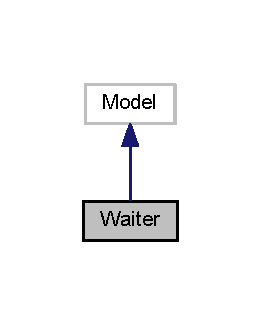
\includegraphics[width=125pt]{class_app_1_1_models_1_1_waiter__inherit__graph}
\end{center}
\end{figure}


Collaboration diagram for Waiter\+:
\nopagebreak
\begin{figure}[H]
\begin{center}
\leavevmode
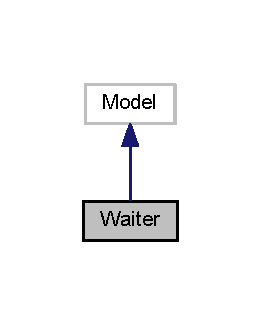
\includegraphics[width=125pt]{class_app_1_1_models_1_1_waiter__coll__graph}
\end{center}
\end{figure}
\subsection*{Protected Attributes}
\begin{DoxyCompactItemize}
\item 
\mbox{\Hypertarget{class_app_1_1_models_1_1_waiter_ae8876a14058f368335baccf35af4a22b}\label{class_app_1_1_models_1_1_waiter_ae8876a14058f368335baccf35af4a22b}} 
{\bfseries \$table} = \textquotesingle{}waiters\textquotesingle{}
\item 
{\bfseries \$fillabe}
\item 
\mbox{\Hypertarget{class_app_1_1_models_1_1_waiter_a4a374564d2858d8ae869a8fb890aad56}\label{class_app_1_1_models_1_1_waiter_a4a374564d2858d8ae869a8fb890aad56}} 
{\bfseries \$hidden} = \mbox{[}\textquotesingle{}password\textquotesingle{}\mbox{]}
\end{DoxyCompactItemize}


\subsection{Detailed Description}
This model represnts a \mbox{\hyperlink{class_app_1_1_models_1_1_waiter}{Waiter}}. A \mbox{\hyperlink{class_app_1_1_models_1_1_waiter}{Waiter}} is not a \mbox{\hyperlink{class_app_1_1_models_1_1_user}{User}}.

Accepts name\+: string, email\+: string, password\+: string, address\+: string, salary\+: double, monthly\+\_\+comission\+: double, comission\+\_\+percentage\+: double monthly\+\_\+orders\+\_\+total\+\_\+value\+: double, admission\+\_\+date\+: Date, demission\+\_\+date\+: Date, status. Status represents if the \mbox{\hyperlink{class_app_1_1_models_1_1_waiter}{Waiter}} is active or not. If not, the logging will always fail. The password is a hidden field, which means the password will not be returned when getting the full object. 

\subsection{Field Documentation}
\mbox{\Hypertarget{class_app_1_1_models_1_1_waiter_ac5c29ce22e45a54200f88204e498d290}\label{class_app_1_1_models_1_1_waiter_ac5c29ce22e45a54200f88204e498d290}} 
\index{App\+::\+Models\+::\+Waiter@{App\+::\+Models\+::\+Waiter}!\$fillabe@{\$fillabe}}
\index{\$fillabe@{\$fillabe}!App\+::\+Models\+::\+Waiter@{App\+::\+Models\+::\+Waiter}}
\subsubsection{\texorpdfstring{\$fillabe}{$fillabe}}
{\footnotesize\ttfamily \$fillabe\hspace{0.3cm}{\ttfamily [protected]}}

{\bfseries Initial value\+:}
\begin{DoxyCode}
= [
        \textcolor{stringliteral}{'name'},
        \textcolor{stringliteral}{'email'},
        \textcolor{stringliteral}{'password'},
        \textcolor{stringliteral}{'address'},
        \textcolor{stringliteral}{'salary'},
        \textcolor{stringliteral}{'monthly\_commission'},
        \textcolor{stringliteral}{'commission\_percentage'},
        \textcolor{stringliteral}{'monthly\_orders\_total\_value'},
        \textcolor{stringliteral}{'admission\_date'},
        \textcolor{stringliteral}{'demission\_date'},
        \textcolor{stringliteral}{'status'}
    ]
\end{DoxyCode}


The documentation for this class was generated from the following file\+:\begin{DoxyCompactItemize}
\item 
app/\+Models/Waiter.\+php\end{DoxyCompactItemize}

\hypertarget{class_app_1_1_http_1_1_controllers_1_1_waiter_controller}{}\section{Waiter\+Controller Class Reference}
\label{class_app_1_1_http_1_1_controllers_1_1_waiter_controller}\index{Waiter\+Controller@{Waiter\+Controller}}


Inheritance diagram for Waiter\+Controller\+:
\nopagebreak
\begin{figure}[H]
\begin{center}
\leavevmode
\includegraphics[width=166pt]{class_app_1_1_http_1_1_controllers_1_1_waiter_controller__inherit__graph}
\end{center}
\end{figure}


Collaboration diagram for Waiter\+Controller\+:
\nopagebreak
\begin{figure}[H]
\begin{center}
\leavevmode
\includegraphics[width=166pt]{class_app_1_1_http_1_1_controllers_1_1_waiter_controller__coll__graph}
\end{center}
\end{figure}
\subsection*{Public Member Functions}
\begin{DoxyCompactItemize}
\item 
\mbox{\hyperlink{class_app_1_1_http_1_1_controllers_1_1_waiter_controller_a5b75ba6bc9debb999c0186a31978ec03}{\+\_\+\+\_\+construct}} (\$repository)
\item 
\mbox{\hyperlink{class_app_1_1_http_1_1_controllers_1_1_waiter_controller_a149eb92716c1084a935e04a8d95f7347}{index}} ()
\item 
\mbox{\hyperlink{class_app_1_1_http_1_1_controllers_1_1_waiter_controller_a4fa811c83f27da01b0d92bdb2a711a13}{create}} (\$request)
\item 
\mbox{\hyperlink{class_app_1_1_http_1_1_controllers_1_1_waiter_controller_ab7b27a90191560dcef32126b0945db0d}{update}} (\$request)
\item 
\mbox{\hyperlink{class_app_1_1_http_1_1_controllers_1_1_waiter_controller_a126a3799c44d72393ca4732081306dfd}{delete}} (\$request)
\end{DoxyCompactItemize}


\subsection{Detailed Description}
\mbox{\hyperlink{class_app_1_1_http_1_1_controllers_1_1_controller}{Controller}} for the waiters. 

\subsection{Constructor \& Destructor Documentation}
\mbox{\Hypertarget{class_app_1_1_http_1_1_controllers_1_1_waiter_controller_a5b75ba6bc9debb999c0186a31978ec03}\label{class_app_1_1_http_1_1_controllers_1_1_waiter_controller_a5b75ba6bc9debb999c0186a31978ec03}} 
\index{App\+::\+Http\+::\+Controllers\+::\+Waiter\+Controller@{App\+::\+Http\+::\+Controllers\+::\+Waiter\+Controller}!\+\_\+\+\_\+construct@{\+\_\+\+\_\+construct}}
\index{\+\_\+\+\_\+construct@{\+\_\+\+\_\+construct}!App\+::\+Http\+::\+Controllers\+::\+Waiter\+Controller@{App\+::\+Http\+::\+Controllers\+::\+Waiter\+Controller}}
\subsubsection{\texorpdfstring{\+\_\+\+\_\+construct()}{\_\_construct()}}
{\footnotesize\ttfamily \+\_\+\+\_\+construct (\begin{DoxyParamCaption}\item[{}]{\$repository }\end{DoxyParamCaption})}

Using dependency injection to get the repository connected to the A\+PI in the app\+\_\+providers.


\begin{DoxyParams}[1]{Parameters}
interface & {\em \$repository} & \\
\hline
\end{DoxyParams}


\subsection{Member Function Documentation}
\mbox{\Hypertarget{class_app_1_1_http_1_1_controllers_1_1_waiter_controller_a4fa811c83f27da01b0d92bdb2a711a13}\label{class_app_1_1_http_1_1_controllers_1_1_waiter_controller_a4fa811c83f27da01b0d92bdb2a711a13}} 
\index{App\+::\+Http\+::\+Controllers\+::\+Waiter\+Controller@{App\+::\+Http\+::\+Controllers\+::\+Waiter\+Controller}!create@{create}}
\index{create@{create}!App\+::\+Http\+::\+Controllers\+::\+Waiter\+Controller@{App\+::\+Http\+::\+Controllers\+::\+Waiter\+Controller}}
\subsubsection{\texorpdfstring{create()}{create()}}
{\footnotesize\ttfamily create (\begin{DoxyParamCaption}\item[{}]{\$request }\end{DoxyParamCaption})}

Store a new waiter.

\begin{DoxyReturn}{Returns}
boolean 
\end{DoxyReturn}
\mbox{\Hypertarget{class_app_1_1_http_1_1_controllers_1_1_waiter_controller_a126a3799c44d72393ca4732081306dfd}\label{class_app_1_1_http_1_1_controllers_1_1_waiter_controller_a126a3799c44d72393ca4732081306dfd}} 
\index{App\+::\+Http\+::\+Controllers\+::\+Waiter\+Controller@{App\+::\+Http\+::\+Controllers\+::\+Waiter\+Controller}!delete@{delete}}
\index{delete@{delete}!App\+::\+Http\+::\+Controllers\+::\+Waiter\+Controller@{App\+::\+Http\+::\+Controllers\+::\+Waiter\+Controller}}
\subsubsection{\texorpdfstring{delete()}{delete()}}
{\footnotesize\ttfamily delete (\begin{DoxyParamCaption}\item[{}]{\$request }\end{DoxyParamCaption})}

Delete a waiter.

\begin{DoxyReturn}{Returns}
boolean 
\end{DoxyReturn}
\mbox{\Hypertarget{class_app_1_1_http_1_1_controllers_1_1_waiter_controller_a149eb92716c1084a935e04a8d95f7347}\label{class_app_1_1_http_1_1_controllers_1_1_waiter_controller_a149eb92716c1084a935e04a8d95f7347}} 
\index{App\+::\+Http\+::\+Controllers\+::\+Waiter\+Controller@{App\+::\+Http\+::\+Controllers\+::\+Waiter\+Controller}!index@{index}}
\index{index@{index}!App\+::\+Http\+::\+Controllers\+::\+Waiter\+Controller@{App\+::\+Http\+::\+Controllers\+::\+Waiter\+Controller}}
\subsubsection{\texorpdfstring{index()}{index()}}
{\footnotesize\ttfamily index (\begin{DoxyParamCaption}{ }\end{DoxyParamCaption})}

Returns all the waiters.

\begin{DoxyReturn}{Returns}
array 
\end{DoxyReturn}
\mbox{\Hypertarget{class_app_1_1_http_1_1_controllers_1_1_waiter_controller_ab7b27a90191560dcef32126b0945db0d}\label{class_app_1_1_http_1_1_controllers_1_1_waiter_controller_ab7b27a90191560dcef32126b0945db0d}} 
\index{App\+::\+Http\+::\+Controllers\+::\+Waiter\+Controller@{App\+::\+Http\+::\+Controllers\+::\+Waiter\+Controller}!update@{update}}
\index{update@{update}!App\+::\+Http\+::\+Controllers\+::\+Waiter\+Controller@{App\+::\+Http\+::\+Controllers\+::\+Waiter\+Controller}}
\subsubsection{\texorpdfstring{update()}{update()}}
{\footnotesize\ttfamily update (\begin{DoxyParamCaption}\item[{}]{\$request }\end{DoxyParamCaption})}

Update a waiter.

\begin{DoxyReturn}{Returns}
boolean 
\end{DoxyReturn}


The documentation for this class was generated from the following file\+:\begin{DoxyCompactItemize}
\item 
app/\+Http/\+Controllers/Waiter\+Controller.\+php\end{DoxyCompactItemize}

%--- End generated contents ---

% Index
\backmatter
\newpage
\phantomsection
\clearemptydoublepage
\addcontentsline{toc}{chapter}{Index}
\printindex

\end{document}
